\documentclass{book}
\usepackage{graphicx} % Required for inserting images

\graphicspath{ {./images/} }
\usepackage{geometry}
\usepackage{hyperref}
\usepackage{amsmath}
\usepackage{amsfonts}
\usepackage{tikz-qtree}
\newgeometry{
left=   1 in,
bottom= 1.5 in,
right=  1 in,
top=    1 in
}


\title{Deep Learning Notes}
\author{Riccardo Cappi}
\date{February 2024}

\begin{document}

\maketitle

\section{Disclaimer}
These are just my notes that I used to prepare for the exam. So, probably, there will be both spelling and conceptual errors. Feel free to contact me at riccardo.cappi@studenti.unipd.it if you find any errors. This is the github repo where you can find the latex files of the notes: \url{https://github.com/riccardocappi/Computer-Science-notes}

\tableofcontents

\chapter{Lec 02-03 Machine Learning Basics}

\section{What is Machine Learning}
\textit{A computer program is said to learn from experience E with respect to some class of tasks T and performance measure P, if its performance at tasks in T, as measured by P, improves with experience E.} Basically, Machine Learning is the field of study that gives computers the ability to learn without being explicitly programmed. In fact, we use Machine Learning when its impossible to \textbf{exactly formalise} the problem (and so to give an algorithmic solution) or when formulating a solution it's very complex and cannot be done manually.
\subsection{Main Learning Paradigms}
\begin{itemize}
    \item \textbf{Supervised Learning:}
    \begin{itemize}
        \item \textbf{Goal: }give the \textit{right answer} for each example in the data.
        \item Given a training set $\{(x^{(i)}, y^{(i)})\}$ we look for a function $h(\cdot)$ which is able to map in a predictive way $x^{(i)}$'s to $y^{(i)}$'s. It's called supervised learning because there is an expert that provides a \textit{supervision} assigning a label $y^{(i)}$ to each input $x^{(i)}$ 
        \item \textbf{Output: }Classification, regression.
        \item Use cases: Object recognition, Predicting pandemic, ... 
    \end{itemize}
    \begin{center}
        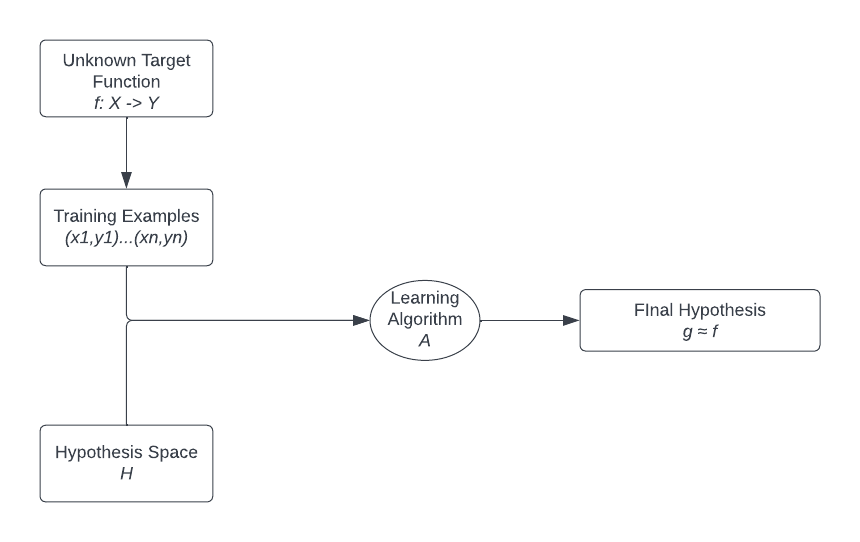
\includegraphics[scale=0.8]{images/Supervised Learning Diagram.png}
    \end{center}
    The \textit{Training examples} are generated according to the \textit{Target function $f$} (unknown). Once we have this set of pairs, we choose the \textit{hypothesis space}. The \textit{learning algorithm} (e.g a Neural Network) searches in the hypothesis space for a function $g$ that approximates the target function $f$.
    \item \textbf{Unsupervised Learning:}
    \begin{itemize}
        \item \textbf{Goal:} Find regularities / patterns on the data
        \item Given examples $\{x^{(i)}\}$, discover regularities on the whole input domain.
        \item There is no supervision.
        \item Use cases: Community detection in social media, user profiling, market analysis ...
    \end{itemize}    
    \item \textbf{Reinforcement Learning:}
    An \textbf{Agent} operates in an environment $e$, which in response to action $a$ (given by the agent) in the state $s$ returns the next state and a reward $r$ (which can be positive, negative or neutral).
    The goal of the Agent is to maximize a reward function.
    \begin{itemize}
        \item Use cases: Robotics, Games, ...
    \end{itemize}
    \begin{center}
        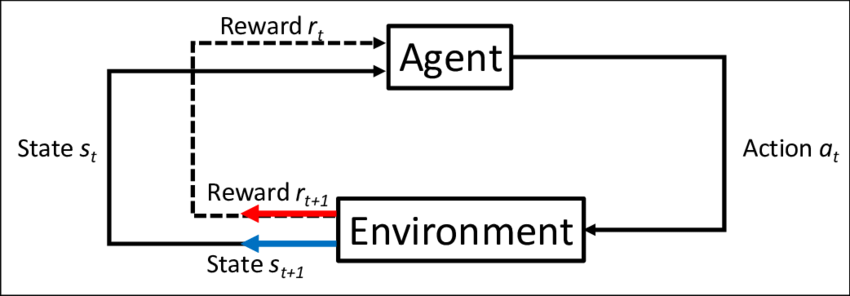
\includegraphics{images/Reinforcement learning.png}
    \end{center}
    \item \textbf{Other Learning Strategies:}
    \begin{itemize}
        \item Active Learning
        \item Online Learning, Incremental \& Continual Learning
        \item Weak Supervised Learning
        \item Self-supervised Learning
        \item Deep Learning and Representation Learning
        \item Federated Learning
    \end{itemize}
\end{itemize}

\subsection{Supervised Learning Keywords}

\begin{itemize}
\item \textbf{Input/Instance space x $\in X$:}
Representation of model's input (e.g. you can choose a Vector as a representation for your input). It contains all the possible inputs for a model. Suppose the model takes in a vector, $input = [x1, x2], x1,x2 \in [1,10]$, then we have $10^2$ possible inputs.
\item \textbf{Output space $y \in Y$:}
In supervised learning we want to perform a prediction based on the input. This prediction can be in the form of:
\begin{itemize}
    \item Binary Classification $y \equiv \{-1, +1\}$
    \item Multi-Class Classification $y \equiv \{1,...,m\}$
    \item Regression $y \equiv \mathbb{R}$
\end{itemize}
\item \textbf{Oracle/Nature:}
It determines how examples are generated. We can have two cases of Oracle
\begin{itemize}
    \item Target function $f: X \rightarrow Y$ It's deterministic and given an object of the input space returns an object of the output space. This function is ideal and \textbf{unknown}.
    \item Probability distribution $P(\textbf{x}), P(y\mid\textbf{x})$ The \textit{selection} of $y$ occurs from a probability distribution. This distribution is still unknown
\end{itemize}
\item \textbf{Training set:}
Set of pairs $\{(\textbf{x}_{1}, y_{1}), ..., (\textbf{x}_{n}, y_{n}) \}$ where each pair is composed by an instance of the input space and it's corresponding label.
\begin{center}
    \begin{tabular}{c|c}
     \textbf{x} & y\\
     000&0  \\
     001&1 \\
     010&1 \\
     .&. \\
     .&. \\
     .&.\\
    \end{tabular}
\end{center}
Data are typically:
\begin{itemize}
    \item Independent: Given two pairs $A,B$ $P(A \mid B) = P(A)$. The choice of one pair is independent from the choice of other pairs.
    
    \item Identically distributed: All pairs are generated by the same probability distribution (the Oracle) $P(\textbf{x},y) = P(\textbf{x})P(y\mid \textbf{x})$. \textit{Concept drift} is when data aren't identically distributed
\end{itemize}
\item \textbf{Hypothesis space:}
A \textbf{predefined} set of hypothesis/functions $H \equiv \{h\mid h:X \rightarrow Y\}$

\item \textbf{Empirical error/risk:}
Discrepancy between the target function $f$ and my approximation of that function $g \in H$ (chosen from the hypothesis space) \textbf{on training data}. For example, in a binary classification problem we can compute empirical error as follows:
\begin{center}
    \[\frac{1}{n}\sum_{i=1}^{n} [\![y_{i}\neq g(\textbf{x}_{i})]\!]\]
\end{center}
where $[\![\cdot]\!]$ is a function that is 1 if $\cdot$ is true and 0 otherwise.

\item \textbf{Ideal error:}
The \textbf{expected} error of hypothesis $h$ with respect to target concept $c$ and distribution $D$ is the probability that $h$ will misclassify an instance drawn according to $D$. This can only be estimated. One way to estimate this quantity is testing the model over new examples that are not in the training set (test set) 

\item \textbf{Inductive bias:}
Since the hypothesis space can't contain all possible functions, we must make assumptions about the type of the unknown target function. The inductive bias consists of:
\begin{itemize}
    \item The hypothesis space: how $H$ is defined
    \item The learning algorithm: how $H$ is explored
\end{itemize}
\textbf{Examples of Inductive bias:}
\begin{itemize}
    \item \textbf{Hyperplanes in} $\mathbb{R}^{2}$: We chose as input space points in the plane $X = \{y\mid y \in \mathbb{R}^{2}\}$, and as hypothesis space the dichotomies induced by hyperplanes in $\mathbb{R}^{2}$, that is, $H = \{f_{w,b}(y) = sign(\textbf{w} \cdot y + b), \textbf{w} \in \mathbb{R}^{2}, b \in\mathbb{R}\}$.
    \begin{center}
        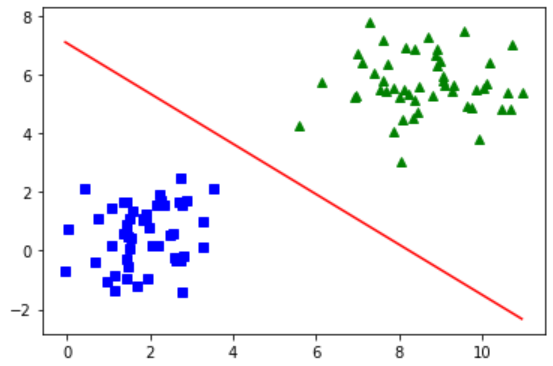
\includegraphics{Hyperplanes in R^2}
    \end{center}

    In this case the assumption is that examples are linearly separable
    
    \item \textbf{Polynomial functions}:
    Given a training set $S = \{(x_{1},y_{1}),...,(x_{n}, y_{n})\}, x\in \mathbb{R}, y\in \mathbb{R}$, the hypothesis space is the one containing functions of type: $h_{w}(x) = w_{0} + w_{1}x + w_{2}x^{2} + ... + w_{p}x^{p}, p\in \mathbb{N}$. The assumption is on the degree $p$ of the polynomial function.
    \begin{center}
        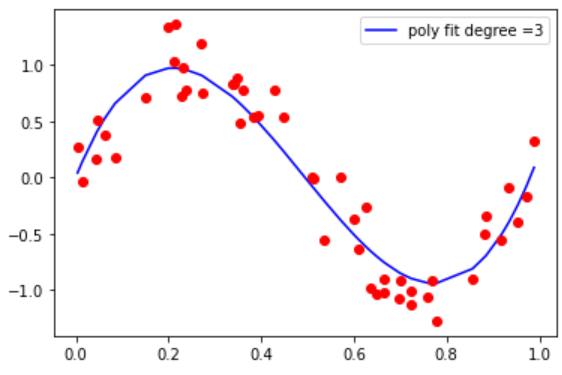
\includegraphics{images/Poly reg.png}
    \end{center}
\end{itemize}
\textbf{Bias-Variance Tradeoff:}
The learning goal is to find the best tradeoff between bias and variance.
\begin{itemize}
    \item The \textbf{bias} error is produced by weak assumptions in the learning algorithm. High bias can cause an algorithm to miss relevant relations between features and target outputs (\textbf{underfitting}).
    \item The \textbf{variance} is an error produced by an over-sensitivity to small fluctuations in the training set. High variance can cause an algorithm to model the random noise in the training data, rather than the intended outputs (\textbf{overfitting}).
    \begin{center}
        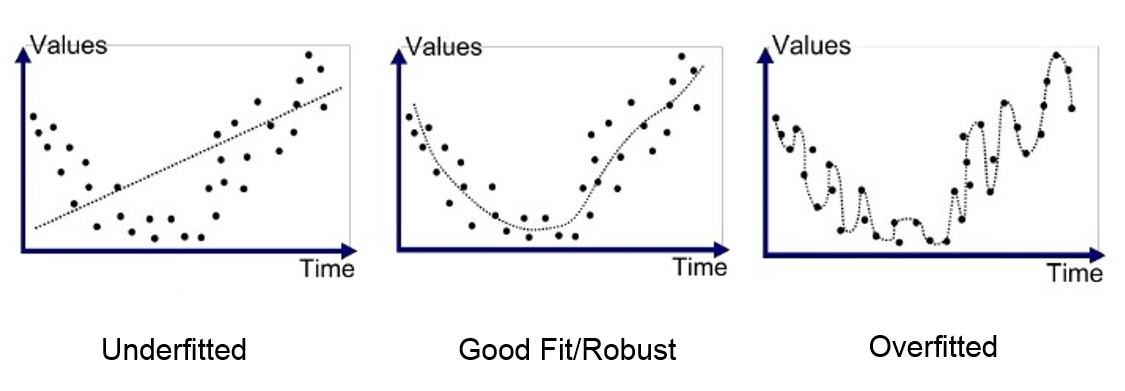
\includegraphics[scale = 0.35]{images/Overfitting vs Underfitting.png}
    \end{center}
\end{itemize}
\end{itemize}

\section{Example of Learning Algorithm: Perceptron}
Consider the space of hyperplanes in $\mathbb{R}^{n}$, where $n$ is the dimension of the input.
\[H = \{f_{(\textbf{w},b)}(\textbf{x}) = sign(\textbf{w} \cdot \textbf{x} + b): \textbf{w,x} \in \mathbb{R}^{n}, b \in \mathbb{R}\}\]
where $\textbf{w}$ is a vector of weights and $b$ is the \textbf{bias} term.\newline\newline
We can redefine $H$ as:
\[H = \{f_{\textbf{w}^{'}}(\textbf{x}^{'}) = sign(\textbf{w}^{'} \cdot \textbf{x}^{'}): \textbf{w}^{'}, \textbf{x}^{'} \in \mathbb{R}^{n+1}\}\]
after the following change of variables:
\[\textbf{w}^{'} = [b, \textbf{w}], \quad \textbf{x}^{'} = [1, \textbf{x}]\]
it follows that:
\[\textbf{w}^{'} \cdot \textbf{x}^{'} = b + \sum_{i = 1}^{n}\textbf{w}_{i}\textbf{x}_{i} = \textbf{w} \cdot \textbf{x} + b\]
Basically, we add a dimension to $\textbf{w}$ and $\textbf{x}$ just to simplify the notation of $H$.
\begin{center}
    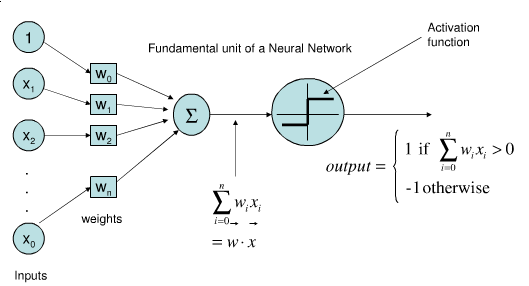
\includegraphics[scale=0.5]{images/perceptron.png}
\end{center}
The model described in the image above is called \textbf{Perceptron}. It first computes the dot-product between the weights $\textbf{w}$ and the input $\textbf{x}$. The result of this computation is usually called $net$
\[net = \sum_{i=0}^{n}w_{i}x_{i}\]
The final output is obtained by applying the \textbf{step function} to the $net$.
\[o = \sigma(net) = sign(net)\]
We will refer to this neuron (and associated learning algorithm) as Perceptron.\newline\newline
Since the hypothesis space of the Perceptron is defined as the hyperplanes in $\mathbb{R}^{n}$, it converges only if the examples in $\mathbb{R}^{n}$ are \textbf{linearly separable}. Otherwise, it will never \textit{find} a hyperplane that separates them.
\subsection{Perceptron: learning algorithm}
Assume to have training examples in $\mathbb{R}^{n}$ that are linearly separable:\newline\newline
Input: Training set $S = \{(\textbf{x}, t), \textbf{x} \in \mathbb{R}^{n+1}, t \in \{-1, +1\}, \eta \geq 0\}$
\begin{enumerate}
    \item Initialize the value of the weights $\textbf{w}$ randomly;
    \item Repeat (N epochs)
    \begin{enumerate}
        \item Select (randomly) one of the training examples $(\textbf{x}, t)$
        \item if $o = sign(\textbf{w} \cdot \textbf{x}) \neq t$ then
        \[\textbf{w} \leftarrow \textbf{w} + \eta(t-o)\textbf{x}\]
    \end{enumerate}
\end{enumerate}
A small value of the learning rate $\eta$ can make the learning process slow but more stable, that is, it prevents sharp changes in the weights vector. If the training set is linearly separable, it can be shown that the Perceptron training algorithm terminates in a finite number of steps.\newline\newline
Let $R$ be the radius of the \textbf{smallest} hyper-sphere centered in the origin enclosing all the instances (how the instances are \textit{spread out}). Let $\gamma$ be the maximal value such that $t_{i}net_{i} = t_{i}(\textbf{w} \cdot \textbf{x}_{i}) \geq \gamma > 0$ (how much the instances are \textit{separated}). Then, it can be shown that the number of steps of the Perceptron algorithm is bounded from above by the quantity $R^{2}/\gamma^{2}$. Basically, bigger \textit{distance} between instances means a smaller number of steps to converge and vice versa.

\section{Model Selection}
Model selection is the process used to compare different models and select the optimal one. In particular, model selection can be performed with respect to different values of the hyper-parameters of a fixed model.\newline\newline
There are several methods used to implement it. A first example can be the so called Hold-out procedure. The idea is to obtain a validation set (or hold-out set) $Va$ by splitting the training set $Tr$. Then, the fixed model is trained using examples in $Tr - Va$, trying different values of the hyper-parameters, and tested against the validation set. This procedure allows you to get an estimate of the error of the model on new unseen data.\newline\newline
Another approach for model selection (and evaluation) is the K-fold cross-validation:
\begin{enumerate}
    \item The training set is partitioned in $k$ disjointed validation sets $Va_{1},...,Va_{k}$. For each classifier $h_{1},...,h_{k}$, we apply the hold-out method on the $k$-th pair, that is, we train $h_{i}$ using examples in $Tr - Va_{i}$ and we test it against $V_{i}$. 

    \item Final error is obtained by individually computing the errors of $h_{1},...,h_{k}$ on the corresponding validation set and averaging the results.
\end{enumerate}
The above procedure is repeated for different values of the hyper-parameters and the predictor with the smallest final error is selected. The special case where $k = |Tr|$ (the validation sets are made of only one example) is called \textbf{leave-one-out} cross-validation.\newline\newline


\chapter{Lec 04-05 - Learning With Gradient Descent}

\section{Gradient-based optimization}
In machine learning we want to maximize/minimize an \textbf{objective function}. This is done by minimizing an \textbf{error function}, which is a measure of the committed error. This optimization problem can be solved exploiting the concepts of derivative and \textbf{gradient}.\newline\newline 
\textbf{Derivative:}\newline
The derivative $f'$ tells us the slope of a function $f$ at any point $x$.
\[f'(x) = lim_{\epsilon \rightarrow 0}\frac{f(x + \epsilon) - f(x)}{\epsilon} \quad \epsilon > 0\]
Given a point:
\begin{itemize}
    \item Positive derivative means that the function increases at that point
    \item Negative derivative means that the function decreases at that point.
    \item Null derivative means that there is a stationary point (minimum, maximum or saddle point).
\end{itemize}
In order to minimize a function in 1 variable, we have to move in the direction \textbf{opposite} to the function derivative.\newline\newline
\textbf{Gradient} is the generalization of derivative with respect to a vector of input variables. In vector calculus, the gradient of a scalar-valued differentiable function $f: \mathbb{R}^{n} \rightarrow \mathbb{R}$ is a vector-valued function $\nabla f: \mathbb{R}^{n} \rightarrow \mathbb{R}^{n}$ whose value at point $p$ is the vector whose components are the partial derivatives of $f$ at $p$.\newline\newline
The gradient vector can be interpreted as the direction and rate of fastest increase of the function. The gradient is the zero vector at a point if and only if the point is a stationary point.
\subsection{Multivariate calculus}
Let's consider a function $f: \mathbb{R}^{2} \rightarrow \mathbb{R}$. It is a function of 2 variables $x_{1}, \,\, x_{2}$ where $x_{1}(t),\,\, x_{2}(t)$ are 2 functions themselves. The derivative of $f$ with respect to $t$ is defined as follows:
\[\frac{d\,f}{d\,t} = \frac{\partial f}{\partial x_{1}}\frac{\partial x_{1}}{\partial t} + \frac{\partial f}{\partial x_{2}}\frac{\partial x_{2}}{\partial t}\]
We can write the formula above in a more convenient way using vectors multiplications:
\[
    \begin{bmatrix}
        \frac{\partial f}{\partial x_{1}}, & \frac{\partial f}{\partial x_{2}} 
    \end{bmatrix}
    \cdot
    \begin{bmatrix}
        \frac{\partial x_{1}(t)}{\partial t}\\
        \vspace{1pt}
        \frac{\partial x_{2}(t)}{\partial t}\\
    \end{bmatrix}
\]
Note that the first term is the gradient of $f$ $\nabla_{\Vec{x}} f$. Note also that $\frac{\partial x_{1}(t)}{\partial t}$ is $\nabla_{t}x_{1}$, and $\frac{\partial x_{2}(t)}{\partial t}$ is $\nabla_t x_2$. We can define $X: \mathbb{R} \rightarrow \mathbb{R}^{2}$ as the following vector:
\[
    \begin{bmatrix}
        x_1 \\
        x_2
    \end{bmatrix}
\]
where $x_1: \mathbb{R} \rightarrow \mathbb{R}$ and $x_2: \mathbb{R} \rightarrow \mathbb{R}$\newline\newline
\textbf{Example:}\newline
$f(x_1, x_2) = x_1^{2} + 2x_2$ where $x_1 = sin(t), \,\, x_2 = cos(t)$
\[
    X(t) = 
    \begin{bmatrix}
        sin(t) \\
        cos(t)
    \end{bmatrix}
\]
\begin{itemize}
    \item $\frac{\partial f}{\partial x_1} = 2x_1$
    \item $\frac{\partial f}{\partial x_2} = 2$
    \item $\frac{\partial x_1}{\partial t} = cos(t)$
    \item $\frac{\partial x_2}{\partial t} = - sin(t)$
\end{itemize}
\[\frac{d \,f}{d\,t} = 2x_1\,cos(t) + 2\,(-sin(t))\]
\[= 2 \, sin(t)cos(t) - 2 \, sin(t)\]
We can do the same thing in matrix notation:
\[\frac{d \, f}{d \, t} = 
    \begin{bmatrix}
        2x_1, & 2
    \end{bmatrix}
    \cdot
    \begin{bmatrix}
        cos(t) \\
        - sin(t)
    \end{bmatrix}
    = 2 \, sin(t)cos(t) - 2 \, sin(t)
\]
\textbf{Example with more than 1 variable:}\newline
Given a function $f(x_1, x_2) = x_1^{2} + 2x_2$, let $g(s, t)$ be the following function:
\[
    g(s, t) = 
    \begin{bmatrix}
        s \cdot sin(t) \\
        s \cdot cos(t)
    \end{bmatrix}
\]
where $g_1 = s \cdot sin(t), g_2 = s \cdot cos(t)$. Let $h$ be the composition between $f$ and $g$:
\[h = f \circ g\]
We want to compute $\frac{d \, h}{d\,(s,t)}$
\[
    \frac{d \, h}{d\,(s,t)} = \frac{\partial f}{\partial \Vec{y}} \cdot \frac{\partial \Vec{y}}{\partial (s, t)} = 
    \begin{bmatrix}
        2x_1, & 2
    \end{bmatrix}
    \cdot
    \begin{bmatrix}
        \frac{\partial g_1}{\partial s}, & \frac{\partial g_1}{\partial t} \\
        \vspace{2pt}\\
        \frac{\partial g_2}{\partial s}, & \frac{\partial g_2}{\partial t}
    \end{bmatrix}
\]
where $\Vec{y} = g(s,t)$
\[
    \frac{d \, h}{d\,(s,t)} =
    \begin{bmatrix}
        2x_1, & 2
    \end{bmatrix}
    \cdot
    \begin{bmatrix}
        sin(t), & s \cdot cos(t)\\
        \vspace{1pt}\\
        cos(t), & -s \cdot sin(t)
    \end{bmatrix}
\]
The collection of all first-order partial derivatives of a vector-valued function $f: \mathbb{R}^n \rightarrow \mathbb{R}^m$ (function $g$ in this case) is called the \textbf{Jacobian Matrix}.

\subsection{Second-order methods}
So far, we have discussed gradients, i.e., first-order derivatives. Sometimes, we are interested in derivatives of higher order. Consider a function $f: \mathbb{R}^2 \rightarrow \mathbb{R}$ of two variables $x, y$.We use the following notation for higher-order partial derivatives (and for gradients):
\begin{itemize}
    \item $\frac{\partial^2 f}{\partial x^2}$ is the second partial derivative of $f$ with respect to $x$.

    \item $\frac{\partial^2 f}{\partial x \partial y}$ is the partial derivative obtained by first partial differentiating with respect to $x$ and then with respect to $y$.
\end{itemize}
The \textbf{Hessian} is the collection of all second-order partial derivative. Generally, for $\textbf{x} \in \mathbb{R}^n$ and $f: \mathbb{R}^n \rightarrow \mathbb{R}$, the Hessian is an $n \times n$ matrix. The Hessian measures the curvature of the function locally around $(x, y)$. If $f: \mathbb{R}^n \rightarrow \mathbb{R}^m$ is a vector field, the Hessian is a $(m \times n \times n)$-tensor. In general, Second order derivatives measure the curvature of a function (concave, convex).
\begin{center}
    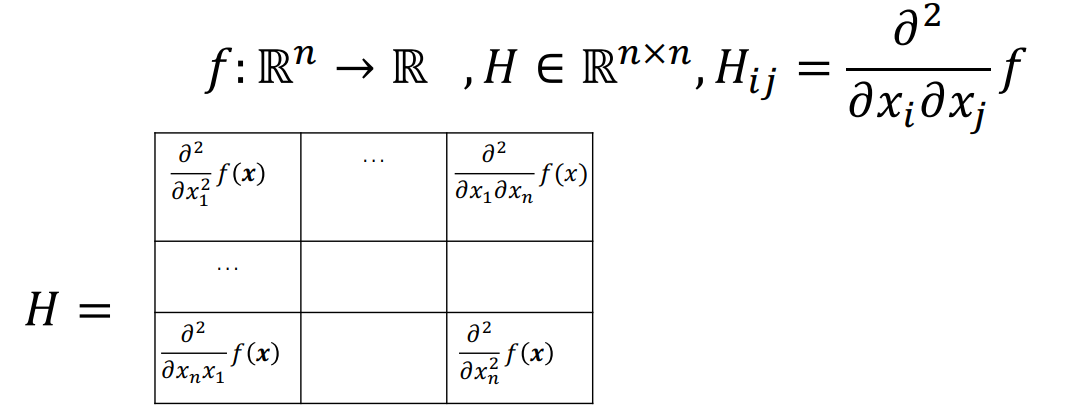
\includegraphics[scale=0.6]{images/hessian.png}
\end{center}
The \textbf{condition number} is the ratio of the maximum and minimum nonzero
eigenvalues of the Hessian matrix. It gives information about the
curvature of a function in the different dimensions. Poorly conditioned problems are long, thin valleys (very curved in one direction, very flat in the other). 
\newline\newline
Second-order optimization algorithm (like Newton’s Method) can be used to solve poorly conditioned problems exploiting the Hessian. However, these methods are slow and therefore they are not widely used for deep learning.

\section{Gradient descent}
Let $f(\textbf{x}): \mathbb{R}^{n} \rightarrow \mathbb{R}$ be a vector-valued function, find the vector $\theta \in \mathbb{R}^{n}$ that minimizes the function $f$:
\[\theta = argmin_{\textbf{x}}f(\textbf{x})\]
This minimization problem can be solved using gradient descent. Starting from a random configuration of $\theta$, each parameter is updated in the following way:
\[\theta_{k+1} = \theta_{k} - \eta \nabla f(\theta_{k})\]
where: 
\begin{itemize}
    \item $\nabla f(\theta_{k})$ is the partial derivative of the function in $\theta_{k}$.
    \item The parameter $\eta > 0$ is known as the \textit{learning rate}. 
\end{itemize}
The derivative term $\frac{\partial}{\partial \theta_{k}}f(\theta_{k})$ can be:
\begin{itemize}
    \item $\geq 0$ it means that the function is increasing, so we are decreasing $\theta_{k}$ in the \textit{right direction}.
    \item $\leq 0$ it means that the function is decreasing, so we are increasing $\theta_{k}$ in the \textit{right direction}
\end{itemize}
If $\eta$ is too small, gradient descent can be slow. Anyway, if it is too large, it can overshoot the minimum (fail to converge).

\section{Example}
Let's consider a simple example of linear regression with a function $h_{\theta}(x) = \theta_{1}x$ and a cost function $J(\theta_{1}) = \frac{1}{2m}\sum_{i = 1}^{m}(h_{\theta}(x^{(i)}) - y^{(i)})^{2}$.
\begin{center}
    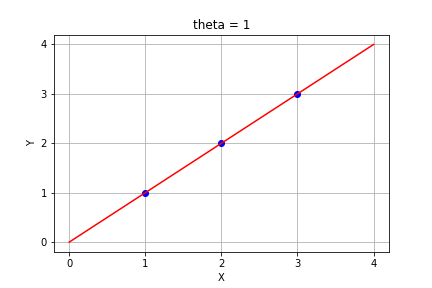
\includegraphics[scale = 0.7]{images/Simple liner reg.png}
\end{center}
As you can see from the graph above, our training set is composed by 3 points $\{(1,1), (2,2), (3,3)\}$. In this simple example the function $h_{\theta}(x)$ that perfectly fits the training set is the one with the parameter $\theta_{1} = 1$. In fact, if we compute the cost function $J(\theta_{1})$ with respect to $\theta_{1} = 1$, the result is 0 (minimized).
\[J(\theta_{1}) = \frac{1}{2m}\sum_{i = 1}^{m}(h_{\theta}(x^{(i)}) - y^{(i)})^{2}\]
\[= \frac{1}{2m}\sum_{i = 1}^{m}(\theta_{1}x^{(i)} - y^{(i)})^{2}\]
\[= \frac{1}{2m}(0+0+0)^2 = 0\]
But let's see what happens for different values of $\theta_{1}$.
\begin{itemize}
    \item $\theta_{1} = \frac{1}{2}$ $J(\theta_{1}) \approx 0.67$
    \item $\theta_{1} = 0$ $J(\theta_{1}) \approx 2.33$
    \item $\theta_{1} = -\frac{1}{2}$ $J(\theta_{1}) \approx 5.25$
\end{itemize}
\begin{center}
    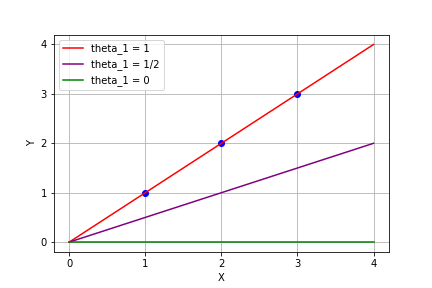
\includegraphics[scale = 0.7]{images/Simple liner reg (colors).png}
\end{center}
Now we can plot the values of $\theta_{1}$ on the \textbf{X} axis and the values of $J(\theta_{1})$ on the \textbf{Y} axis. The shape of $J(\theta_{1})$ will be the following:
\begin{figure}[h]
    \centering
    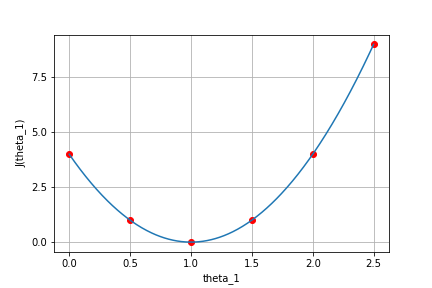
\includegraphics[scale = 0.7]{images/J.png}
    \label{Fig 1}
    \caption{Cost function J}
\end{figure}\newline
We obtain this \textbf{convex} function that has its minimum, for this specific $h_{\theta_{1}}(x^{(i)})$ and $y^{i}$, in 0. This principle is also valid for $n$-dimensional functions but the graphic representation is not that easy.\newline
We can use \textbf{gradient descent} technique in order to find $\theta_{1}$ in an automatic way.
\begin{flushleft}
    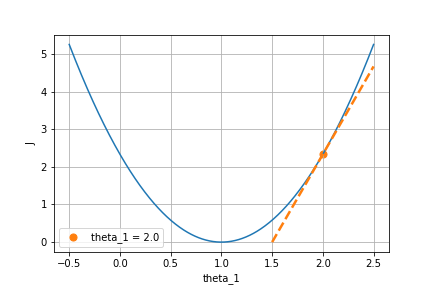
\includegraphics[scale=0.5]{images/partial derivative.png}
    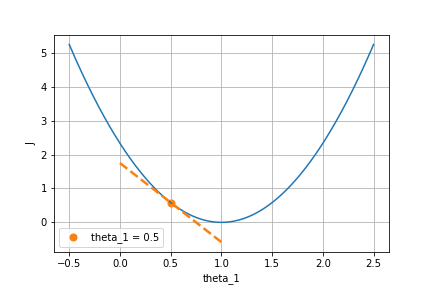
\includegraphics[scale=0.5]{images/partial derivative_1.png}
\end{flushleft}
\begin{center}
    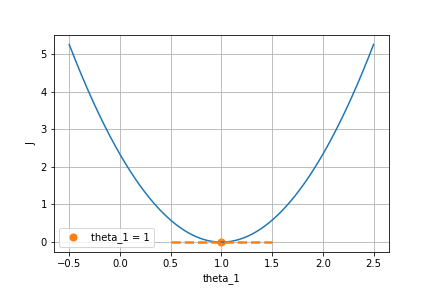
\includegraphics[scale=0.5]{images/partial derivative_2.png}
\end{center}
\textbf{Example of derivation:}\newline\newline
We want to minimize $J[\textbf{w}]$ with respect to the parameters $\textbf{w}$ using gradient descent. Let's start with the derivation of the loss function $J[\textbf{w}]$:
\[\frac{\partial J}{\partial w_{i}} = \frac{\partial}{\partial w_{i}}\left[\frac{1}{2N}\sum_{s=1}^{N}(t^{(s)} - o^{(s)})^{2} \right]\]
\[= \frac{1}{2N} \sum_{s=1}^{N}\frac{\partial}{\partial w_{i}}\left[ (t^{(s)} - o^{(s)})^{2} \right]\]
\[= \frac{1}{2N}\sum_{s=1}^{N}2(t^{(s)} - o^{(s)})\frac{\partial}{\partial w_{i}}\left[ t^{(s)} - o^{(s)}\right]\]
Note that $t^{(s)}$, which is the target value, is a constant that does not depend on $w_{i}$. So, it can be removed from the derivation.
\[= \frac{1}{N} \sum_{s=1}^{N}(t^{(s)} - o^{(s)})\left(-\frac{\partial}{\partial w_{i}}\left[\textbf{w} \cdot \textbf{x}^{(s)}\right]\right)\]
$\textbf{w} \cdot \textbf{x}^{(s)}$ = $w_{1}x_{1}^{(s)} + w_{2}x_{2}^{(s)} + ... + w_{i}x_{i}^{(s)} + ...$. The partial derivative $-\frac{\partial}{\partial w_{i}}\left[\textbf{w} \cdot \textbf{x}^{(s)}\right]$ with respect to  $w_{i}$ is equal to $x_{i}^{(s)}$ because all the other terms are constant. Therefore, the derivation becomes:
\[ = -\frac{1}{N}\sum_{s=1}^{N}(t^{(s)} - o^{(s)})x_{i}^{(s)}\]

\chapter{Lec 06 - Probability}

\section{Probability - terminology}
\begin{itemize}
    \item \textbf{Random variable:} a variable that can take different values randomly

    \item \textbf{Probability distribution:} a description of how likely a random variable x (or a set of random variables) is to take each of its possible states.\newline\newline
    \textbf{Discrete variables:} Probability distribution is described by a \textbf{Probability mass function}
    \begin{itemize}
        \item The domain of $P$ is the set of all possible states of x ($k$ different values).
        
        \item $\forall \, x \in \text{x} \, 0 \leq P(\text{x} = x) \leq 1$
        
        \item $\sum_{x \in \text{x}}P(x) = 1$
    \end{itemize}
    E.g. Uniform distribution $\forall \, x \in \text{x} \, P(\text{x} = x) = \frac{1}{k}$\newline\newline
    \textbf{Continuous variables:} Probability distribution is described by a \textbf{Probability Density Function} (PDF) 
    \begin{itemize}
        \item The domain of $p$ is the set of all possible states of x

        \item $\forall \, x \in \text{x}\, p(x) \geq 0$

        \item $\int p(x) dx = 1$
    \end{itemize}
    E.g. Gaussian distribution

    \item \textbf{Joint probability distribution:} Probability distribution over 2 or more variables $P(\text{x} = x, \text{y} = y)$

    \item \textbf{Gaussian distribution}: The one-dimensional Gaussian with mean $\mu$ and standard deviation $\sigma$ has the following shape:
    \[G(x) = \frac{1}{\sigma \sqrt{2\pi}}e^{-\frac{(x-\mu)^{2}}{2\sigma^{2}}}\]
    \begin{center}
        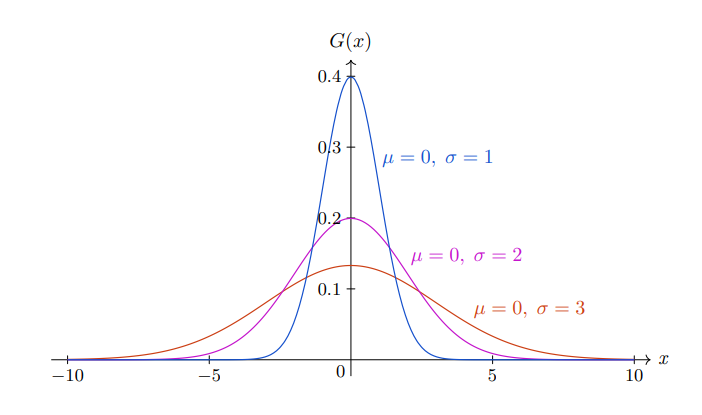
\includegraphics[]{images/Gaussian.png}
    \end{center}

    \item \textbf{Shannon Entropy (discrete variable):} 
    We can apply information theory to calculate the amount of information there is in an event. This is called \textit{self-information} and can be calculated for a \textbf{discrete} event $x$ as follows:
    \[I(x) = -log\,(P(x))\]
    where $log()$ is the base-2 logarithm and $P(x)$ is the probability of the event $x$ \footnote{other bases can be used, $e$ for example}.
    \newline\newline
    The choice of the base-2 logarithm means that the units of the information measure is in bits (binary digits). This can be directly interpreted as the number of bits required to represent an event. If the probability that an event occurs is $0.5$, we need 2 bits two represent it ($0$ fail, $1$ success); if the event occurs with probability $0.125$, we need $3$ bits to represent it (remember $y = log_a\,(x) \iff x = a^y$).
    \newline\newline
    The Shannon entropy of a \textbf{distribution} is the \textbf{expected} amount of information in an event drawn from that distribution:
    \[H(\text{x}) = - E_{x \sim P(\text{x})}[log(P(x))] = -\sum_i P(x_i) log\,P(x_i)\]
    It provides a lower bound on the number of bits needed \textbf{on average} to encode a symbol drawn from the distribution.\newline\newline
    Distributions that are nearly deterministic (where the outcome is nearly certain) have low entropy; distributions that are closer to uniform have high entropy.
    

    \item \textbf{Kullback-Leibler divergence and Cross Entropy:} Let's consider two probability distributions $P(x)$ and $Q(x)$. How can we measure how different they are?
    \begin{itemize}
        \item Kullback-Leiber divergence:
        \[D_{KL}(P \,||\, Q) = E_{x \sim P}\left[ log\frac{P(x)}{Q(x)} \right] = E_{x \sim P}[ log\, P(x) - log\, Q(x)] = \sum_i P(x_i) log\, \left(\frac{P(x_i)}{Q(x_i)}\right)\]
        It is not a true distance because it is not symmetric:
        \[D_{KL}(P \, ||\, Q) \neq D_{KL}(Q \, ||\, P)\]
        It is the measure of information lost when $Q$ is used to approximate $P$.


        \item Cross Entropy:
        \[H(P, Q) = H(P) + D_{KL}(P\, ||\, Q) = -E_{x \sim P}[log\, Q(x)]\]
        where $H(P)$ is the entropy of $P$. Note that minimizing the Cross Entropy of $P$ with respect to $Q$ is equivalent to minimize KL divergence between $P$ and $Q$. (if $P$ is given, $H(P)$ and $E_{x \sim P}[log\, P(x)]$ are constants). If $P$ is a fixed distribution minimize KL divergence or minimize CE is the same, but CE is easier to compute.
    \end{itemize}

    \item \textbf{Maximum likelihood estimation:} Is a principled way to derive estimators (models). Consider $n$ examples $Tr = \{\textbf{x}^{1}, ..., \textbf{x}^{n}\}$ drawn i.i.d. from $p_{data}$ (which is not known in advance). With machine learning we want to estimate this probability $p_{data}$ with some models that depend on a set of parameters $\theta$.\newline\newline
    Let's consider a family of parametric probability distributions (models) $p_{model}(\textbf{x}; \theta)$. It maps a point $\textbf{x}$ to a real number, estimating $p_{data} (\textbf{x})$. How can we find $\theta$ in such a way that $p_{model}$ and $p_{data}$ are as close as possible ? A possible formalization of this problem is given by the Maximum Likelihood estimation for $\theta$:
    \[\theta_{ML} = argmax_{\theta}\, p_{model}(Tr; \theta) = argmax_{\theta}\prod_{i = 1}^{n}p_{model}(\textbf{x}^{i}; \theta)\]
    Basically, we choose the probability distribution which is most likely to have produced our data. Note that we are assuming that all the examples are \textbf{independent} each other ($P(x, y) = P(x)P(y)$).
\end{itemize}

\section{Maximum likelihood}
Maximum likelihood (ML) is a special case of \textbf{maximum a posteriori estimation (MAP)}.
\[h_{MAP} = argmax_{h \in H}P(h|D)\]
\[= argmax_{h \in H}\frac{P(D|h)P(h)}{P(D)}\]
where:
\begin{itemize}
    \item $P(h):$ a priori probability of the hypothesis $h$
    \item $P(D):$ a priori probability of training data. It is the probability to observe exactly this training set when we don't know anything about the hypothesis.
    \item $P(h|D):$ probability of $h$ given $D$. It is the probability that $h$ is the hypothesis that generates data $D$.
    \item $P(D|h):$ probability if $D$ given $h$. Given a hypothesis $h$, it is the probability of data $D$ to be generated by $h$.
\end{itemize}
Since $P(D)$ does not depend on $h$, we can consider it as a constant and remove it from the equation.
\[= argmax_{h \in H}P(D|h)P(h)\]
If we assume uniform probabilities on the hypotheses, that is $P(h_{i}) = P(h_{j})$, we can choose the so called \textbf{maximum likelihood hypothesis} $h_{ML}:$
\[h_{ML} = argmax_{h \in H}P(D|h)\]
MAP and maximum likelihood approach make predictions using a single point estimate of $\theta$. The Bayesian approach is to make predictions using a full probability distribution over $\theta$. For example, given a new instance $\textbf{x}$, which is the most likely \textbf{classification}? The classification given by the most likely hypothesis $h_{MAP}$ is not necessarily the most likely classification. For example, given the following three possible hypothesis:
 \[P(h_{1} | D) = 0.4 \quad P(h_{2} | D) = 0.3 \quad P(h_{3} | D) = 0.3\]
 We want to classify a new instance $\textbf{x}$:
 \[h_{1}(\textbf{x}) = + \quad h_{2}(\textbf{x}) = - \quad h_{1}(\textbf{x}) = -\]
 The most likely hypothesis $h_{1}$ classifies $\textbf{x}$ with the label (+), but the most likely classification is (-). This is because the optimal (Bayes) classification of a certain instance is the class $v_{j} \in V$ which maximizes the following probability:
 \[argmax_{v_{j} \in V} = \sum_{h_{i} \in H}P(v_{j} | h_{i})P(h_{i} | D)\]
 where $V$ is the set of possible labels.\newline\newline
 However, in real-world problems having the probabilities $P(h_{i} | D)$ is almost impossible. Therefore, we usually make the assumption of considering the classification made by $h_{map}$ as most probable.

 \subsection{Maximum likelihood estimation}
 As we said before, the maximum likelihood estimation is defined as follows:
 \[\theta_{ML} = argmax_{\theta}\, p_{model}(Tr; \theta) = argmax_{\theta}\prod_{i = 1}^{n}p_{model}(\textbf{x}^{i}; \theta)\]
 However, computing the product of many probability is unstable. Therefore, we can apply the $log$ and the $argmax$ does not change (log-likelihood).
 \[\theta_{ML} = log(argmax_{\theta}\prod_{i=1}^{n}p_{model}(\textbf{x}^{(i)}; \theta))\]
 \[= argmax_{\theta}\sum_{i = 1}^{n}log\, p_{model}(\textbf{x}^{(i)}, \theta)\]
 We can equivalently divide by $n$ to express maximum likelihood as an expectation over training data:
 \[\theta_{ML} = argmax_{\theta}E_{x \sim \hat{p}_{data}}[log \, p_{model}(x; \theta)]\]
where $\hat{p}_{data}$ is an empirical discrete distribution that we get over the examples in the training set. This implies that maximum likelihood minimizes the dissimilarity between $\hat{p}_{data}$ and $p_{model}$, measured by the KL divergence. It also corresponds to minimize the \textbf{cross-entropy} between the two distributions.

\subsection{Conditional log likelihood}
We can use maximum likelihood to estimate a \textbf{conditional} probability $P(\textbf{y} | \textbf{x}; \theta)$ to predict $\textbf{y}$ given $\textbf{x}$ (supervised learning).
\[\theta_{ML} = argmax_{\theta} P(\textbf{Y} | \textbf{X}; \theta)\]
If input examples are i.i.d.
\[\theta_{ML} = argmax_{\theta}\sum_{i=1}^{n}log\, P(\textbf{y}^{(i)} | \textbf{x}^{(i)}; \theta)\]
Consider any real-valued target function $f$ and learning examples $\langle 
 \textbf{x}_{i}, d_{i}\rangle$ where $d_{i}$ has some noise:
 \begin{itemize}
     \item $d_{i} = f(\textbf{x}_{i}) + e_{i}$
     \item $e_{i}$ is a random variable (noise) extracted independently, for each $\textbf{x}_{i}$, according to a Gaussian distribution with mean 0.
 \end{itemize}
 It can be shown that the maximum likelihood hypothesis is the one that minimizes the mean squared error:
 \[\theta_{ML} = argmin_{\theta} \sum_{i=0}^{m}(d_{i} - \hat{y}_{i})^{2}\]
maximizing the log-likelihood with respect to $\theta$ yields the same estimate of the parameters $\theta$ as does minimizing the mean squared error.

\chapter{Lec 07 - Neural Networks I}

\section{Neural Networks}
An artificial neuron is a unit that computes a non-linear function over the inputs. Its output depends on the input and on the set of \textbf{weights}. These weights have to be learned.\newline\newline
An \textbf{Artificial Neural Network} is a system consisting of interconnected units that compute nonlinear (numerical) functions. Adjustable weights are associated with connections among units.\newline\newline
Deep Feed Forward Neural Networks, also called multi-layer perceptrons (MLP), approximate a function $f^{*}$ that maps an input $x$ to a category $y$. The MLP defines a mapping $\hat{y} = f(x;\theta)$ where $\theta$ is the set of parameters. They are typically represented as a composition of many different functions $f(x) = f^{(3)}(f^{(2)}(f^{(1)}(x)))$. The intermediate layers are called \textbf{hidden layers}, while the final layer is called \textbf{output layer}.\newline\newline
Multiple layers of cascaded units makes a Neural Network able to implement complex non linear functions. The non linearity of the model is given by the activation functions. In fact, without them (linear activation) the result of the model, even if it’s very complex, would still be linear.\newline\newline
\textbf{Example:}\newline
Let's try to define a linear model that predicts the XOR function.
\[Tr = \{ ([0,0], 0), ([0, 1], 1), ([1,0],1), ([1,1], 0)\} \quad f(\textbf{x};\textbf{w};b) = \textbf{x}\textbf{w}^{T} + b\]
The XOR function \textbf{cannot} be learned by any linear classifier. In order to solve this problem, we can define a two-layers Neural Network with the addition of the ReLU activation function $ReLU(y) = max(0, y)$. The networks becomes:
\[f(\textbf{x}; \textbf{W}, \textbf{c}, \textbf{w}, b) = \textbf{w}^{T} \, max(0, \textbf{W}\textbf{x}^{T} + \textbf{c}) + b\]
the following parameters values provide a solution to the XOR problem:
\[
    \textbf{W} =
    \begin{bmatrix}
        1 & 1\\
        1 & 1
    \end{bmatrix},
    \,\,
    \textbf{c} = 
    \begin{bmatrix}
        0 \\
        -1
    \end{bmatrix},
    \,\,
    \textbf{w} = 
    \begin{bmatrix}
        1 \\
        -2
    \end{bmatrix},
    \,\,
    b = 0
\]
Note that the first hidden layer has two nodes.\newline\newline
The most common activation functions are the following:
\begin{center}
    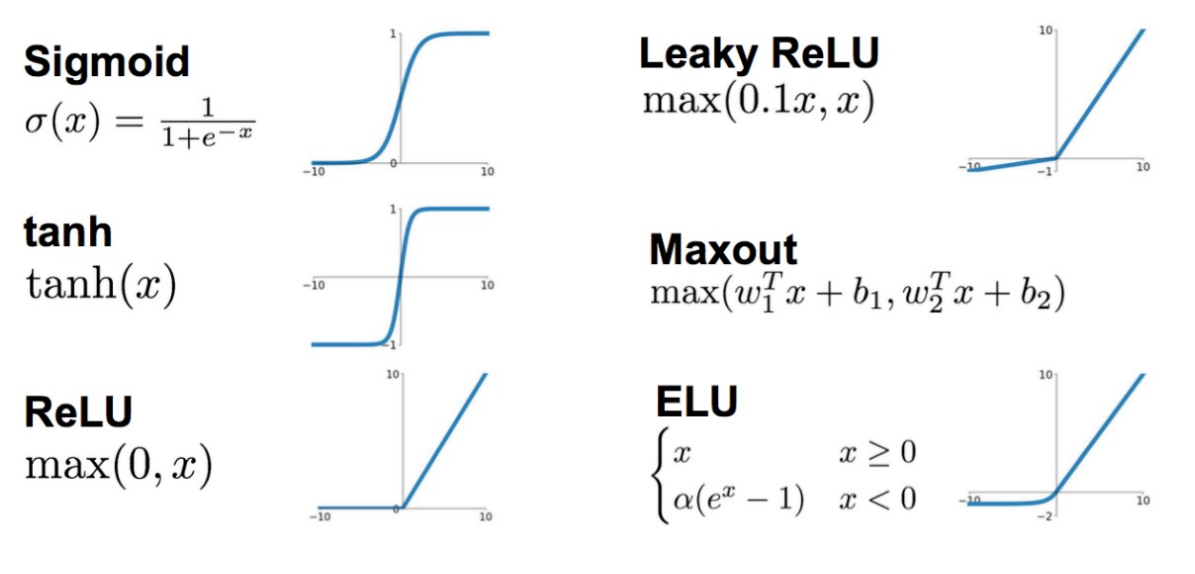
\includegraphics[scale = 0.6]{images/Activation Functions.png}
\end{center}
In general, the goal is to have a more complex decision surface. We can achieve this goal by using non-linear activation functions and stacking several hidden layers. In the XOR example above, the initial points are mapped by the first hidden layer into a new space where they are linearly separable. Thanks to this, the output linear layer is able to classify the points correctly.

\section{Learning in a Neural Network}
In general, the problem of how to update the weights of a model in order to minimize the committed error is called \textbf{credit assignment problem}. A possible solution is to make a single neuron \textbf{derivable} and exploit gradient descent technique to learn the \textit{right} weights. In order to make a neuron derivable, its activation function must be derivable.\newline\newline
Linear models (e.g. SVM) are formulated as \textbf{convex models}. However, the non-linearity in neural networks makes the problem \textbf{non-convex}. It means that there is no guarantee of achieving the global optimum. Furthermore, the way in which the weight of a NN are initialized has a strong impact on the solution that the model will find.

\section{Cost Function}
A important aspect of the design of a deep neural network is the choice of the cost function. In most cases, the model defines a distribution $p(\textbf{y} | \textbf{x}; \theta)$ and the cost function is the cross-entropy between training labels and network predictions (negative log-likelihood):
\[J(\theta) = - E_{(x,y) \sim \hat{p}_{data}}log\, p_{model}(\textbf{y}|\textbf{x})\]
The specific form of the cost function changes from model to model. The output representation $\textbf{h} = f(\textbf{x};\theta)$ determines the form of the cross-entropy function.
\begin{itemize}
    \item \textbf{Linear Regression:} If we assume that the target values are distributed according to a Gaussian distribution $G$, we can think our output layer as to produce the mean of $G$.
    \[\hat{\textbf{y}} = \textbf{W}^{T}\textbf{h} + \textbf{b}\]
    \[G(\textbf{y};\hat{\textbf{y}}; \textbf{I})\]
    As we already seen, in this case maximizing the likelihood corresponds to minimize the mean squared error.
    \[J(\theta) = \frac{1}{2}E_{p \sim \hat{p}_{data}}(y - f(\textbf{x}; \theta))^{2} + constant\]
    Basically, this is a motivation of why the mean squared error cost function is suitable for linear regression.

    \item \textbf{Binary classification:} In this case we assume that our targets are distributed according to a Bernoulli distribution. This distribution depends on a single parameter $\phi \in [0, 1]$:
    \begin{itemize}
        \item $P(\text{x} = 1) = \phi$
        \item $P(\text{x} = 0) = 1 - \phi$
    \end{itemize}
    In general:
    \[P(\text{x} = x) = \phi^{x}(1 - \phi)^{1-x}\]
    The NN just needs to predict $P(\text{y} = 1 | \textbf{x})$. Therefore, we want to force this number to lie in $[0, 1]$. For example, we can use the following function:
    \[P(\text{y} = 1|\textbf{x}) = max(0, min(1, \textbf{w}^{T}\textbf{h} + b))\]
    However, this is not a good choice for gradient descent. In fact, if the output is outside $[0, 1]$ the function is not derivable and the gradient will always be 0. We want to ensure that there is always some gradient when the model is wrong. An alternative way to force the output to lie in $[0, 1]$ is to use an \textbf{output} linear layer with a \textbf{sigmoid activation function}.
    \[\hat{y} = \sigma(\textbf{w}^{T}\textbf{h} + b)\]
    where $\sigma$ is a Sigmoid or Logistic function:
    \[\sigma(x) = \frac{1}{1 + e^{-x}}\]
    \begin{center}
        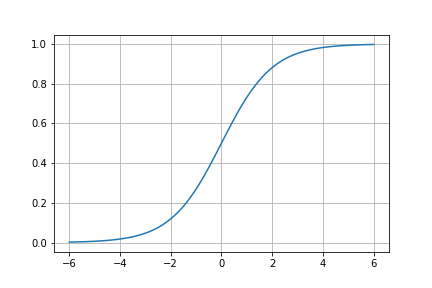
\includegraphics[scale = 0.5]{images/sigmoid.png}
    \end{center}
    An output unit is composed of two components:
    \begin{itemize}
        \item $z = \textbf{w}^{T}\textbf{h} + b$
        \item $\sigma(\cdot)$: the activation function to \textbf{convert $z$ into a probability} (in order to apply maximum likelihood optimization).
    \end{itemize}
    How can we define a probability distribution over $y$ using the value $z$ ? The sigmoid can be motivated by constructing an unnormalized probability distribution $\hat{P}(y)$, which does not sum to 1. We assume that the unnormalized probabilities are linear in $y$ and $z$.
    \[log\, \hat{P}(y) = yz \quad i.e. \,\, log\, \hat{P}(y = 1) = z, \,\, log\, \hat{P}(y = 0) = 0\]
    We can exponentiate to obtain the unnormalized probabilities:
    \[\hat{P}(y) = e^{yz}\]
    Then, we normalize to obtain a proper probablity:
    \[P(y) = \frac{e^{yz}}{\sum_{y'=0}^{1} e^{y'z}} = \sigma((2y - 1)z)\]
    where:
    \begin{itemize}
        \item $P(y = 1) = \frac{1}{1 + e^{-z}}$
        \item $P(y = 0) = \frac{1}{1 + e^{z}}$
    \end{itemize}
    As we already seen, the cost function used with maximum likelihood is the negative-log likelihood. Therefore, the loss function for maximum likelihood learning of a Bernoulli parametrized by a sigmoid is:
    \[J(\theta) = -log\, P(y|\textbf{x}) = -log\,\sigma((2y - 1)z) = \zeta((1 - 2y)z)\]
    where $\zeta(x) = log(1 - exp(x))$ is called \textbf{softplus} function.\newline\newline
    This approach to predicting the probabilities in log-space is natural to use with maximum likelihood learning. The log in the cost function undoes the exp of the sigmoid. Without this effect, the saturation of the sigmoid could prevent gradient- based learning from making good progress.\newline\newline
    The saturation (i.e. when the gradient is very small) occurs when $y = 1$ and $z$ is very positive or $y = 0$ and $z$ is very negative, that is, when the model has the right answer.\newline\newline
    With other cost functions, such as MSE, we'll be able to find a solution but it would \textbf{not} be the maximum-likelihood solution.

    \item \textbf{Multi-class classification:} In this case the output has to be a probability distribution over a discrete variable with $n$ possible values. We have to generate a vector $\hat{\textbf{y}}= [\hat{y}_0, \hat{y}_1, ..., \hat{y}_{n-1}]$ where:
    \begin{itemize}
        \item $\hat{y}_i = P(y = i | \textbf{x})$
        \item $\forall i,\,\, 0 \leq \hat{y}_i \leq 1$
        \item $\sum_i \hat{y}_i = 1$
    \end{itemize}
    We can use the same approach for the Bernoulli distribution generalized to the \textbf{Multinoulli distribution}:
    \[\textbf{z} = \textbf{W}^{T}\textbf{h} + \textbf{b} \quad \text{where}\,\, z_i = log\, \hat{P}(y = i | x)\]
    In order to represent the probability distribution over $n$ different classes, we can use the \textbf{Softmax} function, which is a generalization of sigmoid.
    \[softmax(\textbf{z})_i = \frac{e^{z_i}}{\sum_j^n e^{z_j}}\]
    By applying the log-likelihood, the cost function is:
    \[log\, softmax(\textbf{z})_i = z_i - log \, \sum_j e^{z_j}\]
    $z_i$ pushes the correct labels up and $log \, \sum_j e^{z_j}$ pushes the uncorrect labels down. When we perform the prediction, we'll choose the argmax of $\hat{\textbf{y}}$.
\end{itemize}

\subsection{Output functions in general}
Linear, sigmoid and softmax output units are the most common, but NN can generalize to almost any kind of output layer.\newline\newline
Maximum likelihood provides a guide to design almost any output layer.
\begin{enumerate}
    \item We define a conditional distribution $p(\textbf{y}|\textbf{x}; \theta)$
    \item As cost function, maximum likelihood suggest to use $-log\, p(\textbf{y}|\textbf{x}; \theta)$
\end{enumerate}
We can think of the NN as $f(\textbf{x}; \theta) = \omega$ where $\omega$ are the parameters of a distribution over $\textbf{y}$ and the cost function is $-log\, p(\textbf{y};\omega(\textbf{x}))$

\section{Hidden units}
An hidden unit can be described as accepting an input $x$, computing $z = W^{T}x + b$, and applying an element-wise nonlinear function $g(z)$. The design of hidden units does not have many definitive guiding theoretical principle. What we can do is to evaluate hidden units performance on a validation set. To select the most suitable activation function we can rely on some basic intuitions motivating each type of hidden unit.

\subsection{Hidden units: ReLU}
An hidden unit with ReLU activation function is defined as follows:
\[g(z) = max(0, z) \quad z = f(\textbf{W}^{T}\textbf{x} + \textbf{b})\]
Such hidden units are similar to linear units and therefore easier to optimize. However, ReLU units do not learn via gradient-based methods on examples for which their activation is zero. In order to solve this problem, generalizations of ReLU have been defined (e.g. leakyReLU) $g(z, \alpha)_i = max(0, z_i) + \alpha_i \, min(0, z_i)$.

\subsection{Hidden units: Tanh and sigmoid}
Other common activation functions are Tanh and sigmoid:
\begin{itemize}
    \item Logistic sigmoid: $g(z) = \sigma(z)$
    \item Hyperbolic Tangent: $g(z) = tanh(z) = 2\sigma(2z) - 1$
\end{itemize}
Actually, these two functions are not a very good choice for the hidden layers since they saturate across most of their domain. In particular, they saturate to high value when $z$ is very positive, and to low value when $z$ is very negative. This is good for output units, as we seen before, but not for hidden units, because in hidden layers we just want to keep learning without necessarily having a value between 0 and 1. Tanh typically performs better than the logistic sigmoid.\newline\newline
In general, many differentiable functions are reasonable (e.g. $cos(x)$), but they show no significant advantage over common ones.

\section{Architecture}
The architecture of a NN is its overall structure. Neural networks are generally organised in layers where each layer is a function of the preceding one:
\[\textbf{h}^{(1)} = g^{(1)}(\textbf{W}^{(1)T}\textbf{x} + \textbf{b}^{(1)})\]
\[\textbf{h}^{(i)} = g^{(i)}(\textbf{W}^{(i)T}\textbf{h}^{(i - 1)} + \textbf{b}^{(i)})\]
The main architectural considerations are:
\begin{itemize}
    \item The depth of the network
    \item The width of each layer
\end{itemize}
Deeper networks tend to generalize better, but they are harder to train.\newline\newline
All these hyper-parameters should be validated on a validation set.\newline\newline
\textbf{Universal approximation Theorem}\newline\newline
Given a feed-forward NN with just one hiddel layer, any continuous function $f:\mathbb{R}^{n} \rightarrow \mathbb{R}$ and an arbitrarily small $\epsilon > 0$, then, for a large class of activation functions, there always exists an integer $M$ such that the function $g: \mathbb{R}^{n} \rightarrow \mathbb{R}$ computed by the net using at least $M$ hidden units approximates the function $f$ with tolerance $\epsilon$, that is:
\[max_{x \in \Omega}|f(\textbf{x}) - g(\textbf{x})| < \epsilon\]
Note that the theorem attests the existence of a NN with $M$ hidden units that approximates any continuous function with the desired tolerance, but it says nothing about how $M$ can be computed and how large this network would be. Furthermore, we are not guaranteed that the training algorithm will be able to learn it (the optimization algorithm may not be able to find the value of the parameters that corresponds to the desired function).\newline\newline
Using deeper models can reduce the number of units required to represent the desired function. Furthermore, greater depth does seem to result (empirically) in better generalization for a wide variety of tasks.\newline\newline
Many neural networks architectures have been developed for specific tasks, e.g. Convolutional Neural Networks (CNN) or Recurrent Neural Network (RNN). In general, the layers need to be connected in a chain:
\begin{itemize}
    \item Skip connections: Make it easier for the gradient to flow from output layers to layers nearer the input.

    \item Sparse connections: Each unit in a layer is connected to only a small subset of units in the next layer.
\end{itemize}

\chapter{Lec 08 - Logical Agents}
\section{Logical Agents}
Logical agents simulate the process of \textbf{reasoning} operating on internal \textbf{representations} of knowledge. The problem-solving agents seen so far know things, but only in a very limited,
inflexible sense. The knowledge of what the actions do is hidden inside the domain-specific code of the transition model, which defines the result of a move. We will see that \textbf{logic} provides a possible formalism to support knowledge-based agents.

\section{Knowledge based agents}
The central component of a knowledge-based agent is its \textbf{knowledge base}, or KB. A knowledge base is a set of \textbf{sentences} in a formal language. Each sentence is expressed in a language called a \textbf{knowledge representation language} and represents some assertion about the world.\newline\newline
There must be a way to add new sentences to the knowledge base and a way to query what is known. The standard names for these operations are TELL and ASK, respectively. Both operations may involve inference, that is, deriving new sentences from old.\newline\newline
Agents can be viewed at the \textbf{knowledge level}, that is, what they know, regardless of how implemented, or can be viewed  at the implementation level, data structures in KB and algorithms that manipulate them.
\begin{center}
    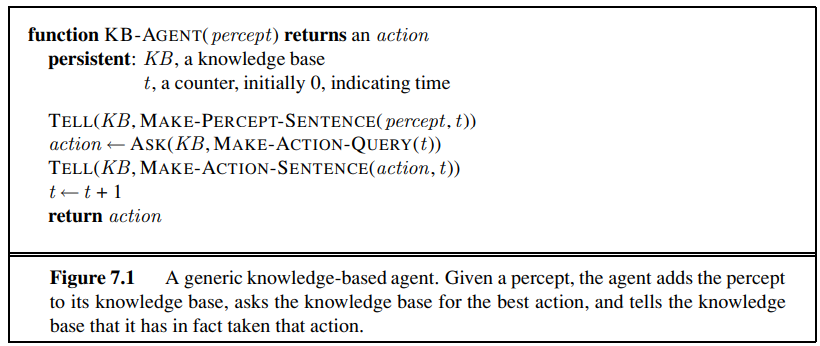
\includegraphics[]{images/KB-agents.png}
\end{center}
The figure above shows the outline of a knowledge-based agent program. Like all our agents, it takes a percept as input and returns an action. The agent maintains a knowledge base, KB, which may initially contain some \textbf{background knowledge}.\newline\newline
Each time the agent program is called, it does three things. First, it TELLs the knowledge base what it perceives. Second, it ASKs the knowledge base what action it should perform. In the process of answering this query, extensive reasoning may be done about the current state of the world, about the outcomes of possible action sequences, and so on.
Third, the agent program TELLs the knowledge base which action was chosen, and the agent executes the action. In order to do so, the agent must be able to:
\begin{itemize}
    \item Represent states, actions, etc.
    \item Incorporate new percepts
    \item Update internal representations of the world
    \item Deduce hidden properties of the world
    \item Deduce appropriate actions
\end{itemize}

\section{The Wumpus world}
In this section we describe an environment in which knowledge-based agents can show their worth. The \textbf{wumpus world} is a cave consisting of rooms connected by passageways. Lurking somewhere in the cave is the terrible wumpus, a beast that eats anyone who enters its room. The wumpus can be shot by an agent, but the agent has only one arrow. Some rooms contain bottomless pits that will trap anyone who wanders into these rooms (except for the wumpus, which is too big to fall in). The only mitigating feature of this bleak environment is the possibility of finding a heap of gold.
\begin{center}
    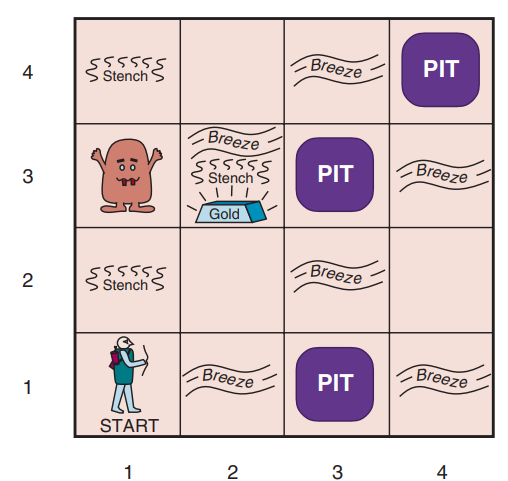
\includegraphics[]{images/wumpus.png}
\end{center}
The precise definition of the task environment is given by the PEAS description:
\begin{itemize}
    \item \textbf{Performance measure}: +1000 for climbing out of the cave with the gold, -1000 for falling into a pit or being eaten by the wumpus, -1 for each action taken and -10 for using up the arrow. The game ends either when the agent dies or when the agent climbs out of the cave.

    \item \textbf{Environment:} A $4 \times 4$ grid of rooms. The agent always starts in the square labeled $[1,1]$, facing to the right. The locations of the gold and the wumpus are chosen randomly, with a uniform distribution, from the squares other than the start square. In addition, each square other than the start can be a pit, with probability 0.2.

    \item \textbf{Actuators:} The agent can move \textit{Forward}, \textit{TurnLeft} by $90^{\circ}$, or \textit{TurnRight} by $90^{\circ}$. The agent dies a miserable death if it enters a square containing a pit or a live wumpus. The action \textit{Grab} can be used to pick up the gold if it is in the same square as the agent. The action \textit{Shoot} can be used to fire an arrow in a straight line in the direction the agent is facing (only one available). Finally, the action \textit{Climb} can be used to climb out of the cave, but only from square $[1,1]$.

    \item \textbf{Sensors:} The agent has five sensors, each of which gives a single bit of information:
    \begin{itemize}
        \item In the square containing the wumpus and in the directly (not diagonally) adjacent squares, the agent will perceive a \textit{Stench}.

        \item In the squares directly adjacent to a pit, the agent will perceive a \textit{Breeze}.

        \item In the square where the gold is, the agent will perceive a \textit{Glitter}.

        \item When an agent walks into a wall, it will perceive a \textit{Bump}.

        \item  When the wumpus is killed, it emits a woeful \textit{Scream} that can be perceived anywhere in the cave.
    \end{itemize}
\end{itemize}
We can characterize the wumpus environment along the various dimensions seen previously. It is discrete, static, and single-agent. It is sequential, because rewards may come only after many actions are taken. It is partially observable, because some aspects of the state are not directly perceivable. For an agent in the environment, the main challenge is its initial ignorance of the configuration of the environment.  Overcoming this ignorance seems to require logical reasoning.\newline\newline
Let us watch a knowledge-based wumpus agent exploring the environment using an informal knowledge representation language consisting of writing
down symbols in a grid:
\begin{center}
    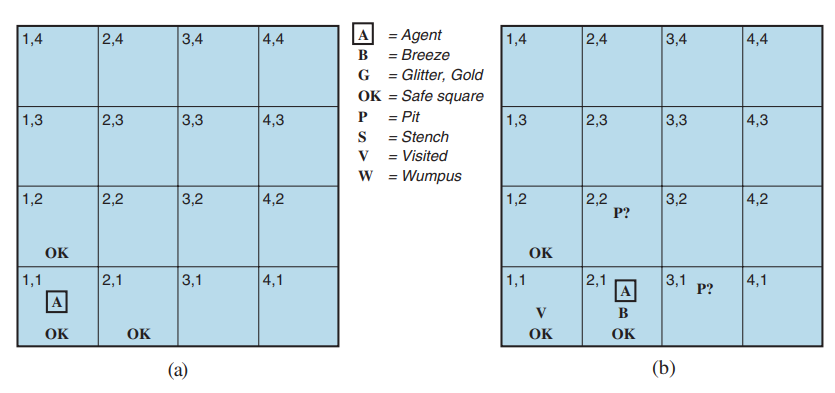
\includegraphics[scale=0.8]{images/wumpus-grid.png}
    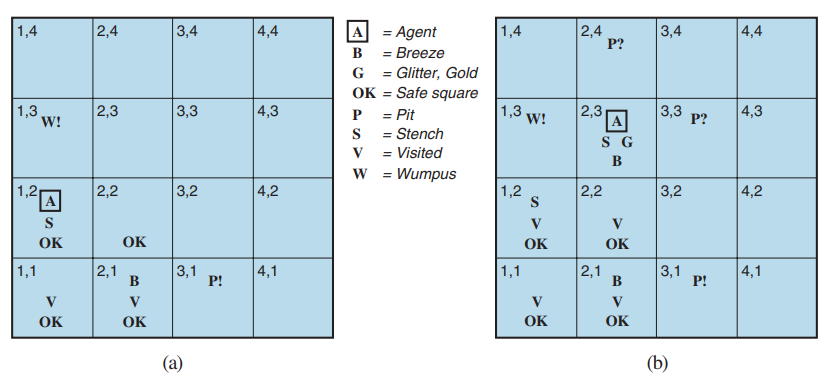
\includegraphics[scale=0.8]{images/wumpus-grid2.png}
\end{center}
Note that in each case for which the agent draws a conclusion from the available information, that conclusion is guaranteed to be correct if the available information is correct. we'll describe how to build logical agents that can represent in a \textbf{formal way} information and draw conclusions.

\section{Propositional Logic}
We now present a simple but powerful logic called \textbf{propositional logic}. The \textbf{syntax} of propositional logic defines the allowable sentences. The \textbf{atomic sentences} consist of a single proposition symbol (P, Q, R, ... but can be whatever). Each such symbol stands for a proposition that can be true or false. There are two proposition symbols with fixed meanings: \textit{True} is the always-true proposition and \textit{False} is the always-false proposition. \textbf{Complex sentences} are constructed from simpler sentences, using parentheses and \textbf{logical connectives}.
\begin{center}
    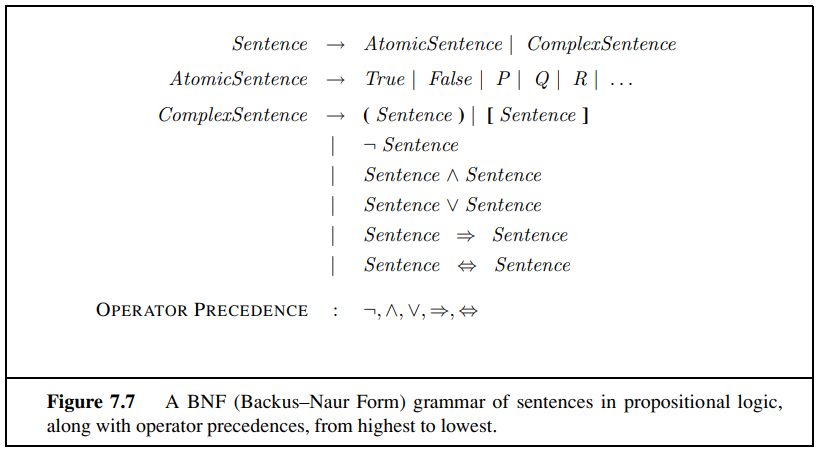
\includegraphics[scale=0.8]{images/BNF.png}
    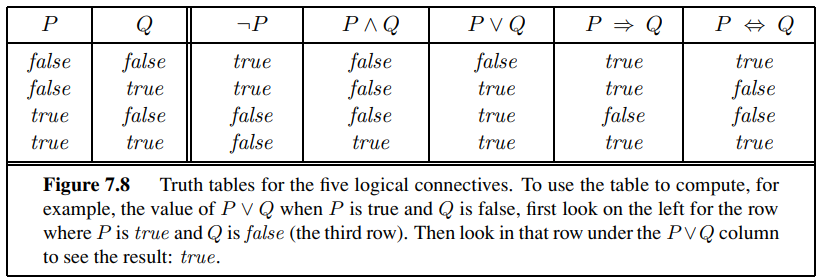
\includegraphics[scale=0.8]{images/truth-table.png}
\end{center}

\section{Models}
As we said previously, the knowledge bases consist of sentences. These sentences are expressed according to the \textbf{syntax} of the representation language, which specifies all the sentences that are well formed. A logic must also define the \textbf{semantics} or meaning of sentences. The semantics defines the truth of each sentence with respect to each possible world.\newline\newline
When we need to be precise, we use the term \textbf{model} in place of “possible world.”  If a sentence $\alpha$ is true in model $m$, we say that $m$ \textbf{satisfies} $\alpha$ or sometimes $m$ \textbf{is a model of} $\alpha$. We use the notation $M(\alpha)$ to mean the set of all models of $\alpha$. Basically, a model assigns truth values to proposition symbols of a sentence.\newline\newline
Now that we have a notion of truth, we are ready to talk about logical reasoning. This involves the relation of logical \textbf{entailment} between sentences, —the idea that a sentence follows logically from another sentence. In mathematical notation, we write:
\[\alpha \vDash \beta\]
to mean that the sentence $\alpha$ entails the sentence $\beta$. The formal definition of entailment is this: $\alpha \vDash \beta$ if and only if, in every model in which $\alpha$ is true, $\beta$ is also true. Using the notation just introduced, we can write
\[\alpha \vDash \beta\,\, \text{if and only if } M(\alpha) \subseteq M(\beta)\]
Note that the direction of the $\subseteq$ means that $\alpha$ is a stronger assertion than $\beta$.\newline\newline
We can apply the same kind of analysis to the wumpus-world reasoning example given previously. The agent has detected nothing in $[1,1]$ and a breeze in $[2,1]$. These percepts, combined with the agent’s knowledge
of the rules of the wumpus world, constitute the KB. The agent is interested (among other things) in whether the adjacent squares $[1,2]$, $[2,2]$, and $[3,1]$ contain pits. Each of the three squares might or might not contain a pit, so (for the purposes of this example) there are $2^3 = 8$ possible models.
\begin{center}
    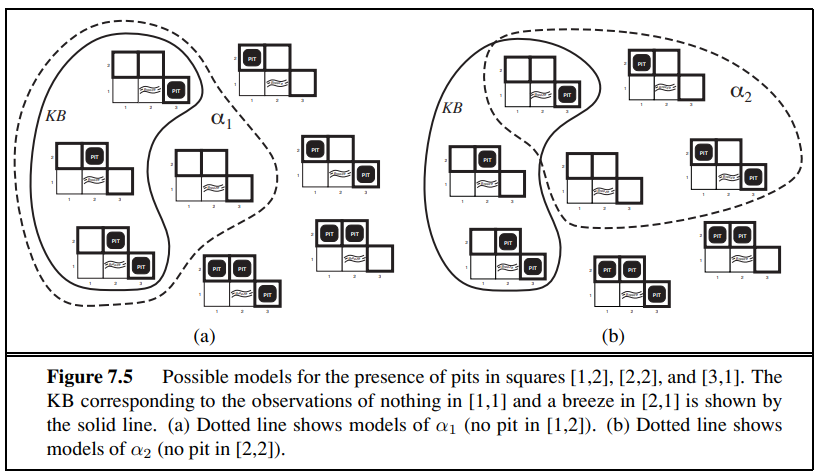
\includegraphics[scale=0.8]{images/kb-wumpus.png}
\end{center}
The KB can be thought of as a set of sentences or as a single sentence that asserts all the individual sentences. The KB is false in models that contradict what the agent knows; for example, the KB is false in any model in which $[1,2]$ contains a pit, because there is no breeze in $[1,1]$. There are in fact just three models in which the KB is true, and these are shown surrounded by a solid line in the figure above.\newline\newline
Now let us consider two possible conclusions:
\begin{itemize}
    \item $\alpha_1 = $ “There is no pit in $[1,2]$.”

    \item $\alpha_2 = $ “There is no pit in $[2,2]$.”

\end{itemize}
By inspection, we see the following: in every model in which KB is true, $\alpha_1$ is also true. Hence $KB \vDash \alpha_1$: there is no pit in $[1,2]$. We can also see that in some models in which KB is true, $\alpha_2$ is false. Hence, the agent cannot conclude that there is no pit in $[2,2]$.\newline\newline
In understanding entailment and inference, it might help to think of the set of all consequences of KB as a haystack and of $\alpha$ as a needle. Entailment is like the needle being in the haystack; inference is like finding it. This distinction is embodied in some formal notation: if an inference algorithm $i$ can derive $\alpha$ from KB, we write:
\[KB \vdash_i \alpha\]
which is pronounced “$\alpha$ is derived from KB by $i$”.\newline\newline
An inference algorithm that derives only entailed sentences is called \textbf{sound}: whenever $KB \vdash_i \alpha$, it is also true that $KB \vDash \alpha$. Note that, as we did with the example before, enumerating all possible models to check that $\alpha$ is true in all models in which KB is true is sound. The property of \textbf{completeness} is also desirable: an inference algorithm is complete if it can derive any sentence that is entailed.\newline\newline
If KB is true in the real world, then any sentence $\alpha$ derived from KB by a sound inference procedure is also true in the real world.

\section{A simple knowledge base}
Now we can construct a knowledge base for the wumpus world, focusing on its immutable aspects. For now, we need the following symbols for each $[x, y]$ location:
\begin{itemize}
    \item $P_{x, y}$ is true if there is a pit in $[x, y]$.
    \item $W_{x,y}$ is true if there is a wumpus in $[x, y]$, dead or alive.
    \item $B_{x,y}$ is true if the agent perceives a breeze in $[x, y]$.
    \item $S_{x,y}$ is true if the agent perceives a stench in $[x, y]$.
\end{itemize}
We label each \textbf{sentence} $R_i$ so that we can refer to them:
\begin{itemize}
    \item There is no pit in $[1,1]$: $R_1:\,\, \neg P_{1,1}$.
    \item A square is breezy if and only if there is a pit in a neighboring square. This has to be stated for each square; for now, we include just the relevant squares:
    \begin{itemize}
        \item $R_2: \,\, B_{1,1} \iff (P_{1,2} \lor P_{2, 1})$
        \item $R_3: \,\, B_{2,1} \iff (P_{1,1} \lor P_{2,2} \lor P_{3,1})$
    \end{itemize}

    \item The preceding sentences are true in all wumpus worlds. Now we include the breeze percepts for the first two squares visited in the specific world the agent is in, leading up to the situation in the figure above (Figure 7.5):
    \begin{itemize}
        \item $R_4: \,\, \neg B_{1,1}$
        \item $R_5: \,\, B_{2,1}$
    \end{itemize}
\end{itemize}
Our goal now is to decide whether $KB \vDash \alpha$ for some sentence $\alpha$. For example, is $\neg P_{1,2}$ entailed by our KB? Our first algorithm for inference is a \textbf{model-checking} approach that is a direct implementation of the definition of entailment: enumerate the models, and check that $\alpha$ is true in every model in which KB is true.
\begin{center}
    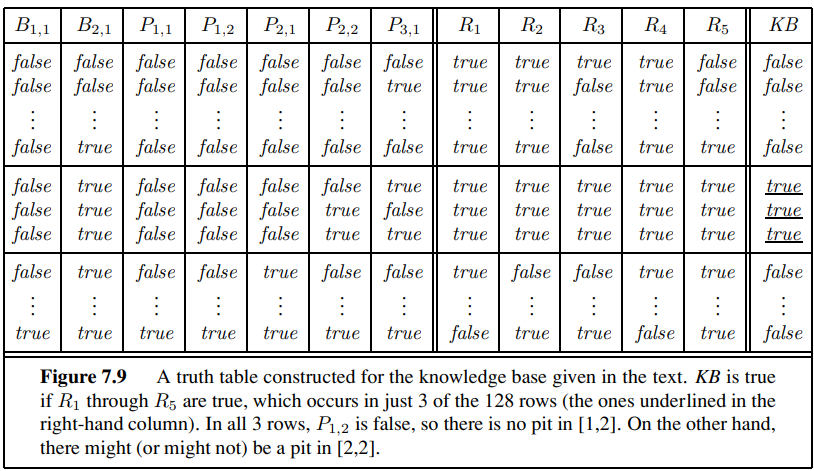
\includegraphics[]{images/wumpus-table.png}
\end{center}
Returning to our wumpus-world example, the relevant proposition \textbf{symbols} are $B_{1,1}, B_{2,1}, P_{1,1}, P_{1,2}, P_{2,1}, P_{2,2}$, and $P_{3,1}$. With seven symbols, there are $2^7 = 128$ possible models; in three of these, KB is true. Note that this is just a "snapshot" of the situation shown in the Figure 7.5. Obviously, as the agent goes on, the KB changes. In the three model where KB is \textit{True}, $\neg P_{1,2}$ is also \textit{True}. Hence, there is no pit in $[1,2]$. On the other hand, $P_{2,2}$ is true in two of the three models and false in one, so we cannot yet tell whether there is a pit in $[2,2]$. Note that KB is true if $R_1$ through $R_5$ are true (KB can be expressed as a sentence $R_1 \land ... \land R_5$), which occurs in just 3 of the 128 rows.
\begin{center}
    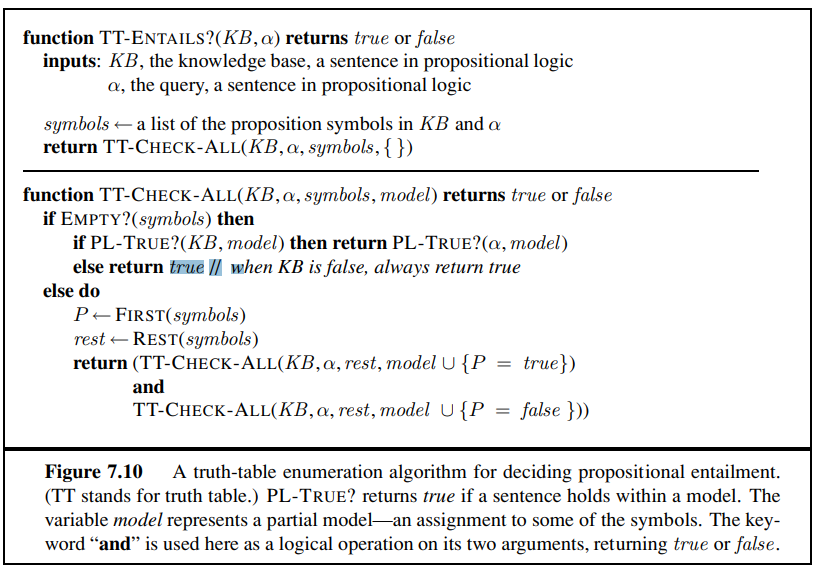
\includegraphics[]{images/tt-algorithm.png}
\end{center}
The algorithm above performs a recursive enumeration of a finite space of assignments to symbols. The algorithm is \textbf{sound} because it implements directly the definition of entailment, and \textbf{complete} because it works for any KB and $\alpha$ and always terminates; there are only finitely many models to examine.\newline\newline
Basically, the algorithm constructs the truth table seen above using a recursive implementation. In particular, it creates a binary tree where the nodes are the symbols in the KB and the branches are truth assignment for that symbol (\textit{True} or \textit{False}). It starts from the first symbol and recursively produces all the possible assignment for all the possible symbols. The paths from the root to the leaves corresponds to the rows of the table above, i.e. the models. Once the algorithm arrives at a leaf, it checks whether the sentence $\alpha$ holds within the corresponding model (path). The algorithm returns always \textit{True} if the KB is \textit{False} w.r.t the model because we are only interested to see if a sentence is \textit{True} when the KB is \textit{True}. These operations correspond to look at the rows of the table (models) where KB is \textit{True} and check whether $\alpha$ is also \textit{True}. If the sentence $\alpha$ is \textit{True} for all the models where also KB is \textit{True} (i.e. all the leaves \textit{returns} \textit{True}), then $\alpha$ can be deduces from KB. Note that if all the leaves return \textit{True}, when the algorithm ascents from recursion, the \textit{True} value is propagated towards the root by the logical \textit{and} and eventually the algorithm returns \textit{True}.  For the same reason, it is sufficient that just one leaf returns \textit{False} that the whole algorithm returns \textit{False} (this is why the algorithms always returns \textit{True} when KB is \textit{False}).\newline\newline
Note that If KB and $\alpha$ contain $n$ symbols in all, then there are $2^n$ models. Thus, the time complexity of the algorithm is $O(2^n)$ (The space complexity is only $O(n)$ because the enumeration is depth-first). Unfortunately, propositional entailment is co-NP-complete.

\chapter{Lec 09-10 - Regularization}

\section{Regularization}
Neural networks are usually \textit{over-parameterized}, that is, they have more parameters than training examples. This implies that the set of parameters can perfectly fit the training data, including the noise (overfitting). In order to limit overfitting, we can perform \textbf{regularization}, that is, any modification we make to a learning algorithm intended to reduce its generalization error but not its training error. Basically, regularization aims at reducing the \textbf{variance} error (favour simpler hypothesis).\newline\newline
Oldest regularization strategies (adopted for linear/logistic regression) limit the capacity of the models, adding a parameter \textbf{norm penalty} to the \textbf{objective function}
\[\tilde{J}(\theta; \textbf{X}; \textbf{y}) = J(\theta; \textbf{X}; \textbf{y}) + \alpha \Omega(\theta)\]
where $\Omega$ is the so called \textbf{regularization term} that depends on the model's parameters. Larger values of the hyper-parameter $\alpha$ results in more regularization. This is because if $\alpha$ is very high, the optimization will favour the second term more than the first and viceversa. In general, only weights are regularized (bias terms tend to be easy to learn).
\begin{center}
    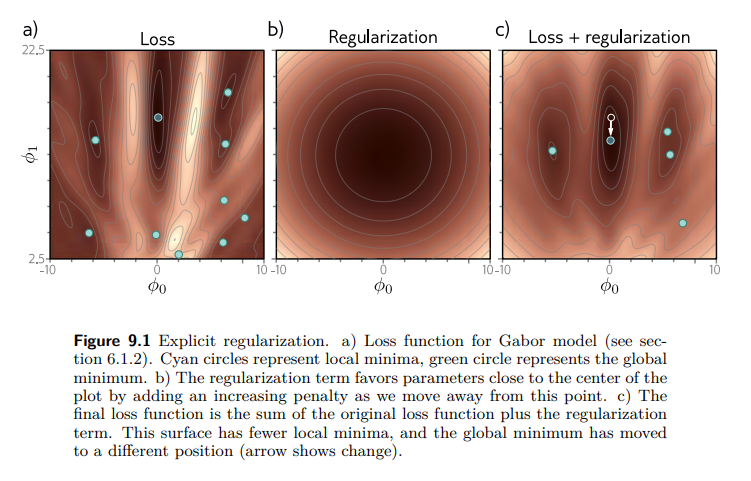
\includegraphics[]{images/Reg.png}
\end{center}
How can we set this regularization term?

\section{Weight decay ($L^2$ norm)}
The idea is to drive the weights close to the origin:
\[\Omega(\theta) = \frac{1}{2} ||w||_2^2\]
where $||w||_2^2$ is the 2-norm of the weight vector ($w^Tw$).\newline\newline
So our new cost function will become:
\[\tilde{J}(\textbf{w}; \textbf{X}, \textbf{y}) = \frac{\alpha}{2}\textbf{w}^T\textbf{w} + J(\textbf{w}; \textbf{X}, \textbf{y})\]
Note that, for simplicity, we are assuming no bias.\newline\newline
Then, we have to compute the gradient of the new cost function with respect to $\textbf{w}$:
\[\nabla_\textbf{w} \tilde{J}(\textbf{w}; \textbf{X}, \textbf{y}) = \alpha \textbf{w} + \nabla_\textbf{w} J(\textbf{w}; \textbf{X}, \textbf{y})\]
A single step of stochastic gradient descent with learning rate $\epsilon$ would be:
\[\textbf{w} \gets \textbf{w} - \epsilon(\alpha \textbf{w} + \nabla_\textbf{w} J(\textbf{w}; \textbf{X}, \textbf{y}))\]
\[\textbf{w} \gets (1 - \epsilon\alpha)\textbf{w} - \epsilon \nabla_\textbf{w} J(\textbf{w}; \textbf{X}, \textbf{y})\]
Basically, we are multiplying the weights vector for a value strictly smaller than 1, so it becomes smaller every SGD step. The weights get shrinked on each step (weight decay). This approach is based on the fact that large weights lead to amplifications of the differences between similar inputs, making the network sensitive, and hence overfitting, to its training data. In contrast, small weights reduce the differences between similar inputs, and hence provides improved generalization.

\subsection{Ordinary Least squares}
Regularization is necessary in some ill-posed ML problems:
\begin{itemize}
    \item When we have less examples than features

    \item Or more in general when the solution is not unique
\end{itemize}
Let's consider linear regression:
\[\textbf{Xw} = \textbf{y}\]
Let's define MSE loss:
\[J(\textbf{w}) = \frac{1}{n}||\textbf{Xw} - \textbf{y}||^2\]
The gradient of $J$ with respect to $\textbf{w}$ is:
\[\nabla_\textbf{w}J = \frac{1}{n}2(\textbf{Xw} - \textbf{y})^T \textbf{X}\]
Now, we can define the closed-form solution equating the derivative to zero:
\[\begin{split}
    \frac{1}{n}2(\textbf{Xw} - \textbf{y})^T \textbf{X} = 0\\
    \textbf{w} = (\textbf{X}^T \textbf{X})^{-1}\textbf{X}^T\textbf{y}
\end{split}\]
Note that $(\textbf{X}^T \textbf{X})^{-1}$ should be invertible, that is, a square full-rank matrix. $\textbf{X}^T \textbf{X}$ is always square, but it is not invertible when the number of variables exceeds the number of data points.\newline\newline
With MSE loss and $L^2$ norm, the gradients would be:
\[\nabla_\textbf{w}J = 2(\textbf{Xw} - \textbf{y})^T \textbf{X} + 2\alpha \textbf{w}^T\]
Therefore, the closed-form solution will be:
\[\begin{split}
    2(\textbf{Xw} - \textbf{y})^T \textbf{X} + 2\alpha \textbf{w}^T = 0\\
    \textbf{w} = (\textbf{X}^T \textbf{X} + \alpha \textbf{I})^{-1}\textbf{X}^T \textbf{y}
\end{split}\]
$(\textbf{X}^T \textbf{X} + \alpha \textbf{I})^{-1}$ is a full-rank matrix and therefore always invertible. The diagonal entries of this matrix correspond to the variance of each input feature, and we add $\alpha$ on this diagonal. We can see that $L^2$ regularization causes the learning algorithm to “perceive” the input $\textbf{X}$ as having higher variance, which makes it shrink the weights on features whose covariance with the output target is low compared to this added variance.


\section{$L^1$ Regularization}
In $L^1$ regularization, $\Omega$ and $\tilde{J}$ are defined as follows:
\[\Omega(\theta) = ||w||_1\]
\[\tilde{J}(\textbf{w}; \textbf{X}, \textbf{y}) = \alpha ||w||_1 + J(\textbf{w}; \textbf{X}, \textbf{y})\]
With gradient $\nabla_\textbf{w}\tilde{J}(\textbf{w};\textbf{X}, \textbf{y}) = \alpha \, sign(\textbf{w}) + \nabla_\textbf{w}J(\textbf{w};\textbf{X}, \textbf{y})$ where $sign(\cdot)$ is applied element-wise. This technique forces the solution to be sparse (i.e. lot of weights to 0 and only few of them $\neq 0$). Therefore, it performs \textbf{feature selection}.\newline\newline
This sparsity property can be seen looking at the gradients formula:
\[\nabla_\textbf{w}\tilde{J}(\textbf{w};\textbf{X}, \textbf{y}) = \alpha \, sign(\textbf{w}) + \nabla_\textbf{w}J(\textbf{w};\textbf{X}, \textbf{y})\]
If $w_i$ is negative, then the term $\alpha \,sign(w_i)$ will be negative and viceversa. Therefore, when we'll perform the update by subtracting the gradients, $w_i$ will be pushed in the opposite direction of its sign by $\alpha$.

\subsection{Geometric interpretation}
Consider a linear regression:
\[\textbf{Xw} = \textbf{y}\]
Given an example in the training set, e.g. $([10, 1], 5)$, we have infinitely many solutions satisfying:
\[\begin{split}
    10 w_1 + w_2 = 5 \\
    w_2 = 5 - 10 w_1
\end{split}\]
\begin{center}
    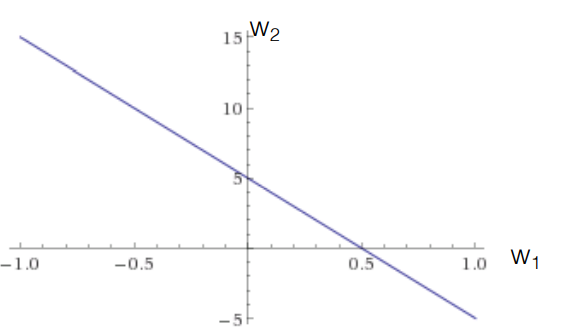
\includegraphics[scale=0.7]{images/geometric l1.png}
\end{center}
This family of solutions (which are infinite) lies on the blue line in the $w_1, w_2$ space represented in the figure above.\newline\newline
The $L^1$ norm is defined as the sum of absolute values:
\[||\textbf{w}||_1 = \sum_i |w_i|\]
In the $w_1, w_2$ space defined previously, all the points with constant $L^1$ norm $c$ lies on a square.
\begin{center}
    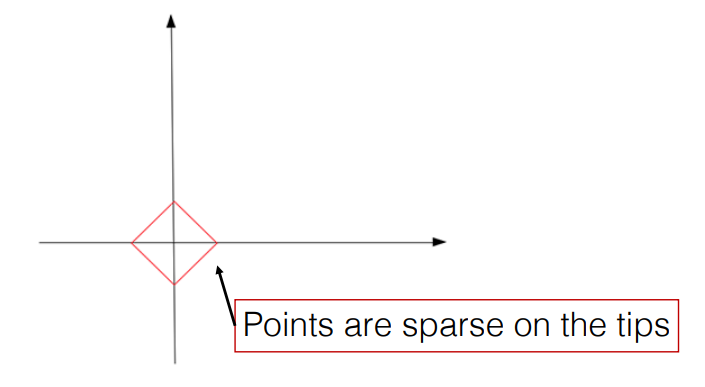
\includegraphics[scale=0.7]{images/l1 reg..png}
\end{center}
If we want to find the solution for $w_2 = 5 - 10 w_1$ with minimum $L^1$ norm, we have to look at the point where it intersects the square.
\begin{center}
    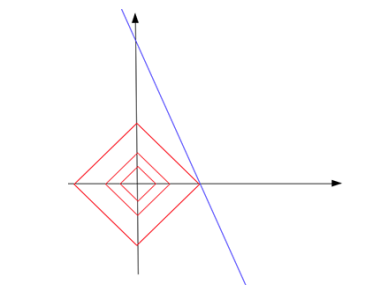
\includegraphics[scale=0.7]{images/l1 sparse.png}
\end{center}
This intersection will probably be on one of the axis, that is, the solution with minimum $L^1$ norm will \textbf{probably} be sparse. This is not always true, but in high-dimensional spaces it is likely.\newline\newline
In the case of $L^2$ norm, instead of a square, the points with constant norm will make a circle (in 2-dimensions). $L^2$ does not enforce sparsity because the solution with minimum norm can be at any point on the circle. Therefore,  $L^2$ causes all the weights to be shrunk towards zero, but none of them are driven to exactly zero.

\section{Data augmentation}
The idea of data augmentation is to generate \textit{fake} training data in order to enrich the training set. For example, in object detection on images, we want the model to be invariant to rotation, translation or scaling; therefore, we can apply some transformations on the training instances in order to achieve this goal.\newline\newline
Another way to perform data augmentation is to inject noise in:
\begin{itemize}
    \item the input examples (e.g. denoising autoencoders)
    \item the hidden representations (e.g. droput)
    \item the target (e.g. label smoothing). Consider a multi-class classification problem. Since the softmax will never give exactly 1 or 0, there will always be a gradient that makes the weights bigger. Label smoothing regularizes a model based on a softmax with $k$ output values by replacing the hard 0 and 1 classification targets with targets of $\frac{\epsilon}{k - 1}$ and $1 - \epsilon$, respectively.\newline\newline
    This technique is also useful if the dataset has some amount of mistakes in the $y$ labels.
\end{itemize}

\section{Semi-supervised learning}
Let's say that we have a problem for which it's easy to gather the data but it's very difficult to set labels for those data. In the paradigm of semi-supervised learning, both unlabeled examples from $P(\textbf{x})$ and labeled examples from $P(\textbf{x}, \textbf{y})$ are used to estimate $P(\textbf{y}|\textbf{x})$ or predict $\textbf{y}$ from
$\textbf{x}$.\newline\newline
We learn a representation $h = f(\textbf{x})$ such that similar examples are close in the new space. A linear classifier in the new space may achieve better generalization. Unsupervised learning can provide useful cues for how to group examples in representation
space.\newline\newline
Instead of having separate unsupervised and supervised components in the model, one can construct models in which a generative model of $P(\textbf{x})$ (autoencoder) shares parameters with a discriminative model of $P(\textbf{y} | \textbf{x})$.

\section{Transfer learning}
When training data is limited, other datasets can be exploited to improve performance. Transfer learning means transferring information from previously learned tasks for the learning of new tasks. Basically, we can take a model that was trained on a similar task and adapt it to our problem. In the case of Neural Networks, we can do this by removing the last layer of the network and adding one or more layers in order to produce a suitable output. The main model may be fixed and the new layers trained for the new task, or we may fine-tune the entire model.\newline\newline
Transfer learning can be viewed as initializing most of the weights of the final network in a sensible part of the space that is likely to produce a good solution.

\section{Multi-Task learning}
Multi-task learning (MTL) is a subfield of machine learning in which multiple learning tasks are solved at the same time. Part of the model is shared across different tasks, and is driven to learn a representation that generalizes well.

\section{Self-supervised learning}
When no data from other tasks is available, we can create large amounts of \textit{free} labeled data using self-supervised learning and use this for transfer learning. For example:
\begin{itemize}
    \item \textbf{generative} self-supervised learning: part of each data example is masked and the learning task is to predict the missing part.

    \item \textbf{contrastive} self-supervised learning: two versions of each unlabeled example are presented, when one has been distorted in some way. The system is trained to predict which is the original.
\end{itemize}

\section{Early stopping}
When training large models with sufficient representational capacity to overfit
the task, we often observe that training error decreases steadily over time, but
validation set error begins to rise again. This means we can obtain a model with better validation set error (and thus, hopefully, better test set error) by returning the model's parameters at the point in time with the lowest validation set error. When the training algorithm terminates, we return these parameters, rather than the latest parameters. The training algorithm terminates when no parameters have improved over the best recorded validation error for some pre-specified number of iterations.\newline\newline
Early stopping acts as a regularizer because it has the effect of
restricting the optimization procedure to a relatively small volume of parameter space in the neighborhood of the initial parameter values.

\section{Parameter Tying and sharing}
Sometimes we might not know precisely what values the parameters should take but we know, from knowledge of the domain and model architecture, that there should be some dependencies between the model parameters.\newline\newline
A common type of dependency that we often want to express is that certain parameters should be close to one another. Consider the following scenario: we have two models performing the same classification task (with the same set of classes) but with somewhat different input distributions. Let us imagine that the tasks are similar enough that we believe the model parameters should be close to each other. We can leverage this information
through regularization. Specifically, we can use a parameter norm penalty of the form:
\[\Theta (w^{(A)}, w^{(B)}) = ||w^{(A)} - w{(B)}||^2_2\]
Basically, it is a regularization term penalizing distant parameters. While a parameter norm penalty is one way to regularize parameters to be close to one another, the more popular way is to use constraints: to force sets of parameters to be equal. This method of regularization is often referred to as
\textbf{parameter sharing}, because we interpret the various models or model components as sharing a unique set of parameters.\newline\newline
By far the most popular and extensive use of parameter sharing occurs in convolutional neural networks (CNNs) applied to computer vision. The same feature is computed over different locations in the input. This means that we can find a cat with the same cat detector whether the cat appears at column $i$ or column $i + 1$ in the image.

\section{Sparse representation}
We have seen $L^1$ regularization to induce weight sparsity. We can similarly induce \textbf{representation sparsity} by placing a penalty on the activations of the units in a neural network, encouraging their activations to be sparse.
\[\Omega(\textbf{h}) = ||\textbf{h}||_1 = \sum_i|h_i|\]
Representational sparsity, on the other hand, describes a
representation where many of the elements of the representation are zero (or close to zero).

\section{Ensemble methods}
The idea of ensemble learning is to get predictions from multiple models and aggregate them. In the classification case, an \textbf{ensemble} of classifiers (base/weak learners) is a set of classifiers whose individual decisions are combined in some way (e.g. majority voting) to classify new examples. Without sufficient data, many hypotheses can have the same level of accuracy on the training data. By "\textit{averaging}" the classifications of several good classifiers the risk of choosing the wrong classifier is reduced.\newline\newline
\textbf{Bagging:}
\begin{enumerate}
    \item Create $k$ bootstrap samples:
    \item Train a distinct classifier on each sample;
    \item Classify new instances by majority voting / average.
\end{enumerate}
For example, considering a linearly separable training set, we can train a perceptron on each bootstrap sample. At the end, we'll obtain a number of perceptrons equals to the number of samples and we can take the majority voting of their predictions.\newline\newline
Ideally, bagging eliminates variance while keeping the bias almost unchanged. Bagging fails when models are very similar (not independent enough). This happens if the learning algorithm is stable, that is, it doesn't change much after changing a few instances. If we have high-bias models and we want to combine them, the result tends to be bad. These methods are more suitable when we want to minimize the variance error.\newline\newline
\textbf{Boosting:}
\begin{itemize}
    \item Use the training set to train a simple predictor;
    \item Re-weight the training examples giving more weight to examples that were wrongly classified;
    \item Repeat $n$ times;
    \item Combine the simple hypotheses into a single accurate predictor.
\end{itemize}
Boosting reduces \textbf{bias} (zero error on training set) by making each classifier focus on previous mistakes.
\subsection{Dropout}
Dropout can be thought of as an efficient method of performing bagging on neural network. Specifically, dropout trains the ensemble consisting of all sub-networks that can be formed by removing non-output units from an underlying base network. We can effectively remove a unit from a
network by multiplying its output value by zero.\newline\newline
To train with dropout, we use a minibatch-based learning algorithm that makes small steps, such as stochastic gradient descent. Each time we load an example into a minibatch, we randomly sample a different binary mask to apply to all of the input and hidden units in the network. The probability of sampling a mask value of one (causing a unit to be included) is a hyperparameter fixed before training begins. Typically, an input unit is included with probability 0.8 and a hidden unit is included with probability 0.5. We then run forward propagation, back-propagation, and the learning update as usual.\newline\newline
More formally, suppose that a mask vector $\mu$ specifies which units to include, and $J(\theta, \mu)$ defines the cost of the model defined by parameters $\theta$
and mask $\mu$. Then dropout training consists in minimizing $E_\mu J(\theta, \mu)$. We can obtain an unbaiased estimate by sampling $\mu$ for each training step.\newline\newline
Dropout training is not quite the same as bagging training. In the case of
bagging, the models are all independent. In the case of dropout, the models share parameters, with each model inheriting a different subset of parameters from the parent neural network.\newline\newline
To make a prediction, a bagged ensemble must accumulate votes from all of
its members. We refer to this process as \textbf{inference} in this context. In the case of bagging, each model $i$ produces a probability distribution $p^{(i)}(y | \textbf{x})$. The prediction of the ensemble is given by the arithmetic mean of all of these distributions:
\[\frac{1}{k}\sum_{i = 1}^{k}p^{(i)}(y | \textbf{x})\]
In the case of dropout, each sub-model defined by mask vector $\mu$ defines a probability distribution $p(y | \textbf{x}, \mu)$. The arithmetic mean over all masks is given by:
\[\sum_{\mu}p(\mu)p(y | \textbf{x}, \mu)\]
where $p(\mu)$ is the probability distribution that was used to sample $\mu$ at training time.\newline\newline
Because this sum includes an exponential number of terms, it is intractable to evaluate. Instead, we can approximate the inference with sampling, by averaging together the output from many masks. Even 10-20 masks are often sufficient to obtain good performance.\newline\newline
However, there is an even better approach, that allows us to obtain a good
approximation to the predictions of the entire ensemble, at the cost of only one forward propagation. To do so, we change to using the geometric mean rather than the arithmetic mean of the ensemble members’ predicted distributions. The unnormalized probability distribution defined directly by the geometric mean is given by:
\[\tilde{p}_{ensemble}(y | \textbf{x}) = \sqrt[2d]{\prod_{\mu} p(y | \textbf{x}, \mu)}\]
where $d$ is the number of units that may be dropped. To make predictions we must re-normalize the ensemble:
\[p_{ensemble}(y | \textbf{x}) = \frac{\tilde{p}_{ensemble}(y | \textbf{x})}{\sum_{y'}p_{ensemble}(y' | \textbf{x})}\]
A key insight involved in dropout is that we can approximate $p_{ensemble}$ by evaluating $p(y | \textbf{x})$ in one model: the model with all units, but with the weights going out of unit $i$ multiplied by the probability of including unit $i$.  The motivation for this modification is to capture the right expected value of the
output from that unit. We call this approach the \textbf{weight scaling inference rule}. There is not yet any theoretical argument for the accuracy of this approximate inference rule in deep nonlinear networks, but empirically it performs very well.\newline\newline
Because we usually use an inclusion probability of $\frac{1}{2}$, the weight scaling rule usually amounts to dividing the weights by 2 at the end of training, and then using the model as usual.\newline\newline
For many classes of models that do not have nonlinear hidden units, the weight scaling inference rule is exact. For example, consider a softmax regression classifier with $n$ input variables represented by the vector $\textbf{x}$:
\[P(\text{y} = y | \textbf{x}) = softmax(\textbf{W}^T \textbf{x} + \textbf{b})_y\]
We can index into the family of sub-models by element-wise multiplication of the input with a binary vector \textbf{d}:
\[P(\text{y} = y | \textbf{x}) = softmax(\textbf{W}^T (\textbf{x} \odot \textbf{d}) + \textbf{b})_y\]
It can be proved that the following holds:
\[\tilde{P}_{ensemble}(\text{y} = y | \textbf{x}) \propto exp(\frac{1}{2}\textbf{W}^T_{y,:}\textbf{x} + b_y)\]

\section{Adversarial training}
In order to probe the level of understanding that a network has of the underlying task, we can search for examples that the model misclassifies. Even neural networks that perform at human level accuracy have a nearly 100\% error rate on examples that are intentionally constructed to mislead the model. These examples are created by using an optimization procedure which searches for an input $\textbf{x}'$ near a data point $\textbf{x}$ such that the model output is very different at $\textbf{x}'$. In many cases, $\textbf{x}'$ can be so similar to $\textbf{x}$ that a
human observer cannot tell the difference between the original example and the \textbf{adversarial example}, but the network can make highly different predictions. Adversarial examples have many implications, for example, in computer security. They are also interesting in the context of regularization because one can reduce the error rate on the original test set via adversarial training, that is, training on adversarially perturbed example from the training set.
\begin{center}
    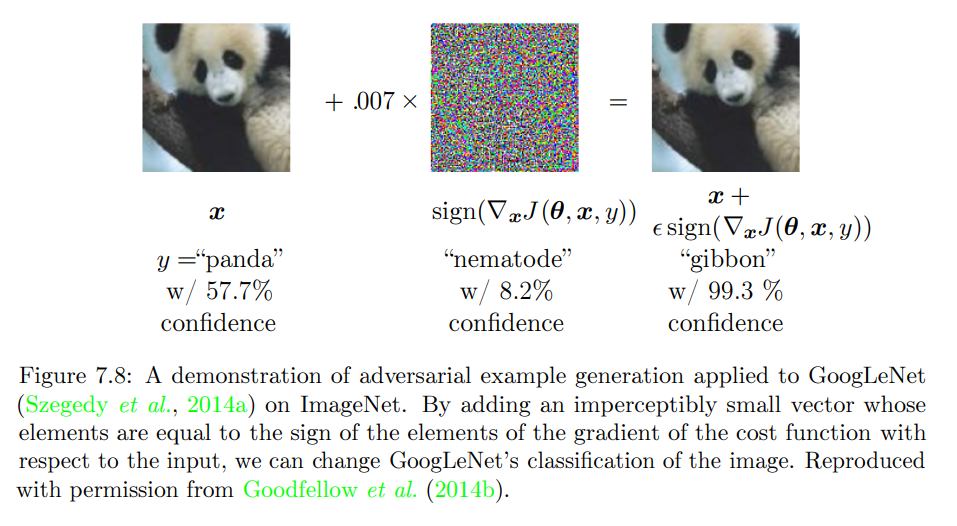
\includegraphics[scale=0.8]{images/Adversarial.png}
\end{center}


\chapter{Lec 11 - 12 - Optimization}

\section{Optimization for Neural Networks}
Optimization algorithms used for training of deep models differ from traditional optimization algorithms in several ways. In most machine learning scenarios, we care about some performance measure
$P$, that is defined with respect to the test set and may also be intractable. We therefore optimize $P$ only \textbf{indirectly}. We reduce a different cost function $J(\theta)$ in the hope that doing so will improve $P$.\newline\newline
The goal of a machine learning algorithm is to reduce the expected generalization error:
\[J^*(\theta) = E_{(\textbf{x}, y) \sim p_{data}} L(f(\textbf{x}; \theta), y)\]
This quantity is known as the \textbf{risk}. If we knew the true distribution
$p_{data}(\textbf{x}, y)$, risk minimization would be an optimization task solvable by an optimization algorithm. However, when we do not know $p_{data}(\textbf{x}, y)$ but only have a training set of samples, we have a machine learning problem. The simplest way to convert a machine learning problem back into an optimization problem is to minimize the expected loss on the training set. This means replacing the true distribution $p(\textbf{x}, y)$ with the empirical distribution $\hat{p}(\textbf{x}, y)$ defined by the training set. We now minimize the \textbf{empirical risk}:
\[E_{(\textbf{x}, y) \sim \hat{p}_{data}} L(f(\textbf{x}; \theta), y) = \frac{1}{m}\sum_{i=1}^m L(f(\textbf{x}^{(i)}; \theta), y^{(i)})\]
where $m$ is the number of training examples. We optimize the empirical risk, and hope that the risk decreases significantly as well \footnote{A variety of theoretical results establish conditions under which the true risk can be expected to decrease by various amounts}. However, empirical risk minimization is prone to overfitting. Models with high capacity can simply memorize the training set. Furthermore, the most effective modern optimization algorithms are based on gradient descent, but many useful loss functions, such as 0-1 loss, have no useful derivatives.

\subsection{Surrogate Loss}
Sometimes, the loss function we actually care about (e.g. classification error) is not one that can be optimized efficiently. For example, exactly minimizing expected 0-1 loss is typically intractable (exponential in the input dimension), even for a linear classifier. In such situations, one typically optimizes a surrogate loss function instead, which acts as a proxy, but has advantages. For example, the negative log-likelihood of the correct class is typically used as a surrogate for the 0-1 loss.\newline\newline
A very important difference between optimization in general and optimization
as we use it for training algorithms is that training algorithms do not usually halt at a local minimum. A machine learning algorithm usually minimizes a surrogate loss function but halts when a convergence criterion based on early stopping is satisfied (whenever overfitting begins to occur).

\subsection{Batch and Minibatch algorithms}
One aspect of machine learning algorithms that separates them from general
optimization algorithms is that the objective function usually decomposes as a sum over the training examples.\newline\newline
Most of the properties of the objective function $J$ used by most of the optimization algorithms are expectations over the training set. For example, the most commonly used property is the gradient:
\[\nabla_\theta J(\theta) = E_{(\textbf{x}, y) \sim \hat{p}_{data}} \nabla_\theta log\,\, p_{model}(\textbf{x}, y; \theta)\]
Computing this expectation exactly is very expensive because it requires
evaluating the model on every example in the entire dataset. In practice, we can compute these expectations by randomly sampling a small number of examples from the dataset, then taking the average over only those examples.\newline\newline
This is motivated by the fact that the standard error of the mean estimated from $n$ samples is given by $\sigma/ \sqrt{n}$, where $\sigma$ is the true standard deviation of the value of the samples. Note that the denominator of $\sqrt{n}$ shows that there are less than linear returns to using more examples to estimate the gradient. Compare two hypothetical
estimates of the gradient, one based on 100 examples and another based on 10,000 examples. The latter requires 100 times more computation than the former, but reduces the standard error of the mean only by a factor of 10.\newline\newline
Most optimization algorithms converge much faster (in terms of total computation, not in terms of number of updates) if they are allowed to rapidly compute approximate estimates of the gradient rather than slowly computing the exact gradient.\newline\newline
Another consideration motivating statistical estimation of the gradient from a small number of samples is redundancy in the training set. In the worst case, all  $m$ samples in the training set could be identical copies of each other. A sampling based estimate of the gradient could compute the correct gradient with a single sample, using $m$ times less computation than the naive approach. Furtherore, small batch size have a regularization effect (introduces noise in the gradient). Gradient-based optimization algorithms can be implemented in three ways:
\begin{itemize}
    \item \textbf{(Full, batch) gradient descent}: computes the gradient of the Loss on the whole training set and then updates the weights.

    \item \textbf{(Online) Stochastic gradient descent} computes the gradient of the Loss on a \textbf{single} example of the training set and then updates the weights.

    \item \textbf{Mini-batch Stochastic gradient descent} computes the gradient of the Loss on a subset of examples (mini-batch) of the training set and then updates the weights

\end{itemize}

\section{Challenges in Neural Network Optimization}

\subsection{Ill- conditioning of Hessian}
A very general problem in numerical optimization is ill-conditioning of the Hessian matrix $\textbf{H}$. Ill-conditioning can manifest by causing SGD to get “stuck” because gradient does not carry enough information about the curvature of the loss function. Even small steps in the gradient direction may result in an increase of the cost function.\newline\newline
The condition number is the ratio between the highest eigenvalues and the lowest eigenvalues. The eigenvalues of the Hessian provides information about the curvature of the loss function in different directions around a point. In particular, the maximum eigenvalue determines the maximum second
derivative and the minimum eigenvalue determines the minimum second derivative.
\newline\newline
When the Hessian has a poor (large) condition number, it means the curvature of the loss function along some direction is much higher than the curvature along some other direction (in the case of a quadratic cost function, this means having a shape like a thin valley).\newline\newline
Gradient descent is unaware of this change in curvature, so it does not know that it needs to explore preferentially in the direction where the derivative remains negative for longer.\newline\newline
In the case of the quadratic cost function mentioned above, if the step size is not small enough, gradient descent may waste time by repeatedly descending these "canyon walls" since it overshoots the minimum.\newline\newline
Second order methods may solve these problems, but they’re not widespread in neural networks training.

\subsection{Local minima}
One of the most prominent features of a convex optimization problem is that it
can be reduced to the problem of finding a local minimum. Any local minimum is guaranteed to be a global minimum. When optimizing a convex function, we know that we have reached a good solution if we find a critical point of any kind. With non-convex functions, such as neural nets, it is possible to have many local minima. This could be a problem because they can be associated with a high value loss, being far away from the global minimum. Since the derivative in these points is 0, gradient-based optimization algorithms may be stuck in a sub-optimal solution. This is valid also for other kind of critical points such as saddle points, local maxima and flat regions. However, as we will see, local minima is not necessarily a major problem, since new research suggest that, for large enough nn, local minima have generally low cost.\newline\newline
To check if we reached a critical point, we can plot the norm of the gradient:
\begin{center}
    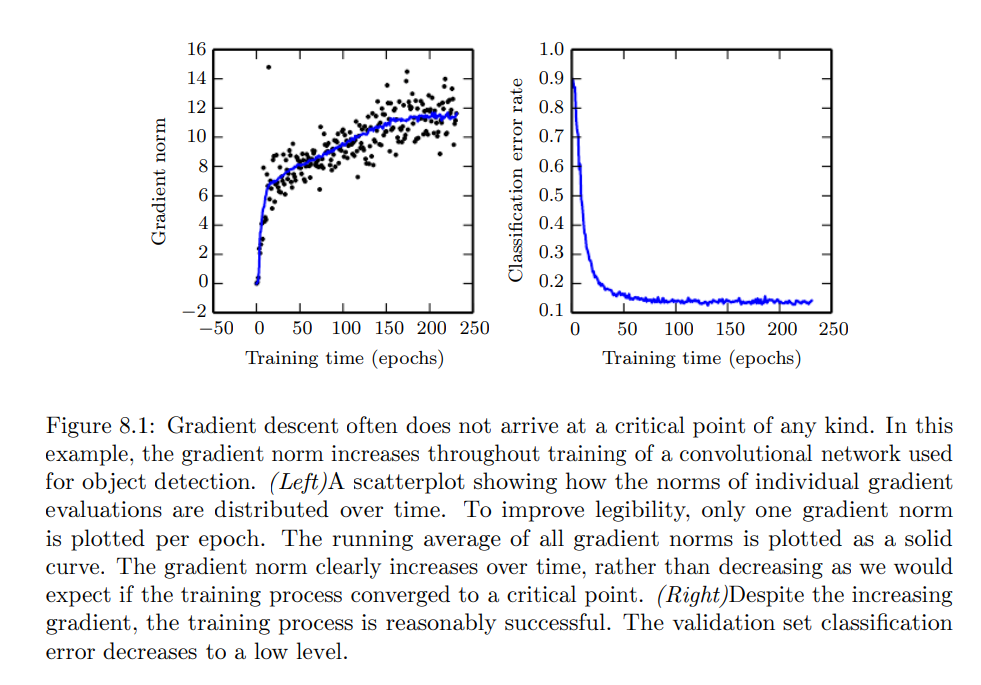
\includegraphics[scale=0.8]{images/Gradient norm.png}
\end{center}

\subsection{Saddle points}
Many classes of random functions exhibit the following behavior: in low dimensional spaces, local minima are common. In higher dimensional spaces, local minima are rare and saddle points are more common. More formally, For a function $f : \mathbb{R}^n \rightarrow \mathbb{R}$ of this type, the expected ratio of the number of saddle points to local minima grows exponentially with $n$. To understand the intuition behind this behavior, observe that the Hessian matrix at a local minimum has only positive eigenvalues. The Hessian matrix at a saddle point has a mixture of positive and negative eigenvalues. In $n$-dimensional space, it is exponentially unlikely that all eigenvalues are positive.\newline\newline
Fortunately, the eigenvalues of the Hessian become more likely to be positive as we reach regions of lower cost. This means that local
minima are much more likely to have low cost than high cost. This happens also for neural networks.\newline\newline
For first-order optimization algorithms that use only gradient information, the gradient can often become very small near a saddle
point. On the other hand, gradient descent empirically seems to be able to escape saddle points in many cases.\newline\newline
For Newton’s method, it is clear that saddle points constitute a problem. Gradient descent is designed to move \textit{downhill} and is not explicitly designed to seek a critical point. Newton’s method, however, is designed to solve for a point where the gradient is zero. Without appropriate modification, it can jump to a saddle point.\newline\newline
There are other kinds of points with zero gradient besides minima and saddle points. There are also maxima, which are much like saddle points from the perspective of optimization—many algorithms are not attracted to them, but unmodified Newton’s method is. Maxima of many classes of random functions become exponentially rare in high dimensional space, just like minima do.\newline\newline
There may also be wide, flat regions of constant value. In these locations, the gradient and also the Hessian are all zero.

\subsection{Cliffs and exploding gradients}
Neural networks with many layers often have extremely steep regions resembling cliffs. On the face of an extremely steep cliff structure, the gradient update step can move the parameters extremely far, usually jumping off of the cliff structure altogether. Fortunately, its most serious consequences can be avoided using the \textbf{gradient clipping} heuristic. The basic idea is to reduce the step size to be small enough that it is less likely to go outside the region
where the gradient indicates the direction of approximately steepest descent.

\subsection{Exploding/Vanishing gradient}
Another difficulty that neural network optimization algorithms must overcome
arises when the computational graph becomes extremely deep. Feedforward
networks with many layers have such deep computational graphs. So do \textbf{recurrent networks}, which construct very deep computational graphs by repeatedly applying the same operation at each time step of a long temporal sequence. Repeated application of the same parameters gives rise to the \textbf{vanishing and exploding gradient problem}. Vanishing gradients make it difficult to know which direction the parameters should move to improve the cost function, while exploding gradients can make learning unstable. The cliff structures described earlier that motivate gradient clipping are an example of the exploding gradient phenomenon.\newline\newline
The vanishing gradient problem can occur also with activation functions that can saturate (e.g. sigmoid) providing gradient close to zero \footnote{basically, weights are no longer updated since the gradient is too small}.\newline\newline
Recurrent networks use the same matrix \textbf{W} at each time step, but feedforward networks do not, so even very deep feedforward networks with non-saturating activation functions (e.g. ReLU) can largely avoid the vanishing and exploding gradient problem.

\subsection{Inexact gradients}
Most optimization algorithms are designed with the assumption that we have
access to the exact gradient or Hessian matrix. In practice, we usually only have a noisy or even biased estimate of these quantities. Nearly every deep learning algorithm relies on sampling-based estimates using a minibatch of training examples to compute the gradient.\newline\newline
In other cases, the objective function we want to minimize is actually intractable. When the objective function is intractable, typically its gradient is intractable as well. In such cases we can only approximate the gradient.\newline\newline
Various neural network optimization algorithms are designed to account for
imperfections in the gradient estimate. One can also avoid the problem by choosing a surrogate loss function that is easier to approximate than the true loss.

\subsection{Local structure not representative of global structure}
Many of the problems we have discussed so far correspond to properties of the loss function at a single point—it can be difficult to make a single step if $J(\theta)$ is poorly conditioned at the current point $\theta$, or if $\theta$ lies on a cliff, or if $\theta$ is a saddle point hiding the opportunity to make progress downhill from the gradient. Optimization based on local downhill moves can fail if the local surface does not point toward the global solution.
\begin{center}
    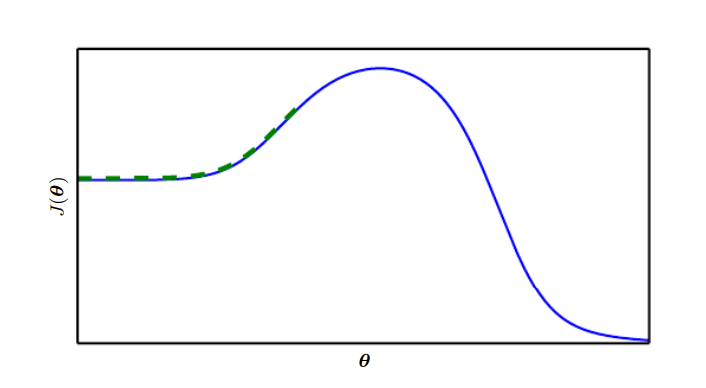
\includegraphics[]{images/bad-init.png}
\end{center}
Much of research into the difficulties of optimization has focused on whether training arrives at a global minimum, a local minimum, or a saddle point, but in practice neural networks do not arrive at a critical point of any kind. The problem in this case is bad initialization.\newline\newline
Many existing research directions are aimed at finding \textbf{good initial points} for problems that have difficult global structure, rather than developing algorithms that use non-local moves. Gradient descent and essentially all learning algorithms that are effective for training neural networks are based on making small, local moves.

\section{Basic Optimization algorithm}
\subsection{Stochastic Gradient Descent}
Stochastic gradient descent (SGD) and its variants are probably the most used optimization algorithms for machine learning in general and for deep learning in particular.
\begin{center}
    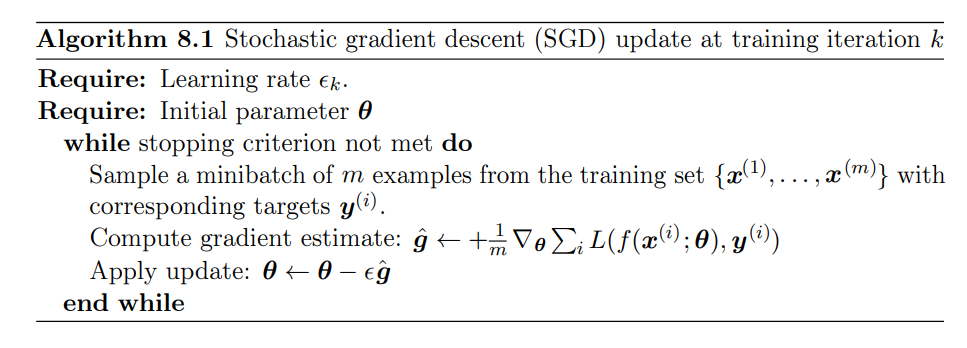
\includegraphics[scale=0.8]{images/SGD.png}
\end{center}
A crucial parameter for the SGD algorithm is the learning rate. In practice, it is necessary to gradually decrease the learning rate over time, so we now denote the learning rate at iteration $k$ as $\epsilon_k$. This is because the SGD gradient estimator introduces a source of noise (the random sampling of m training examples) that does not vanish even when we arrive at a minimum. The true gradient approaches 0 in a minimum, the stochastic estimate doesn’t, so batch gradient descent can use a fixed learning rate. In practice, it is common to decay the learning rate linearly until iteration $\tau$:
\[\epsilon_k = (1 - \alpha)\epsilon_0 + \alpha \epsilon_\tau\]
with $\alpha = \frac{k}{\tau}$. After iteration $\tau$, it is common to leave $\epsilon_\tau$ constant.  
\begin{center}
    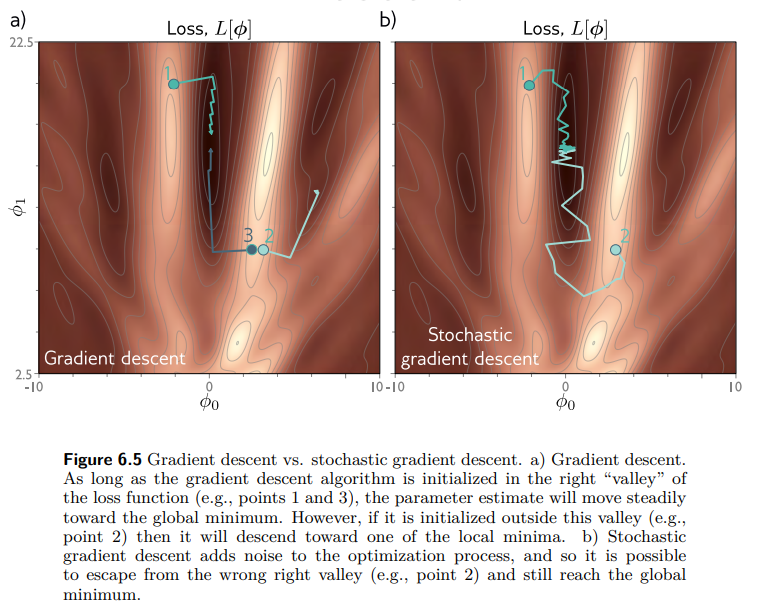
\includegraphics[scale=0.8]{images/SGD vs BGD.png}
\end{center}

\subsection{Momentum}
While stochastic gradient descent remains a very popular optimization strategy, learning with it can sometimes be slow. The method of \textbf{momentum} is designed to accelerate learning, especially in the face of high curvature, small but consistent gradients, or noisy gradients. Furthermore, the problem with gradient descent is that the weight update at a moment ($t$) is governed by the learning rate and gradient at that moment only. It does not take into account the past steps taken while traversing the cost space.
\begin{center}
    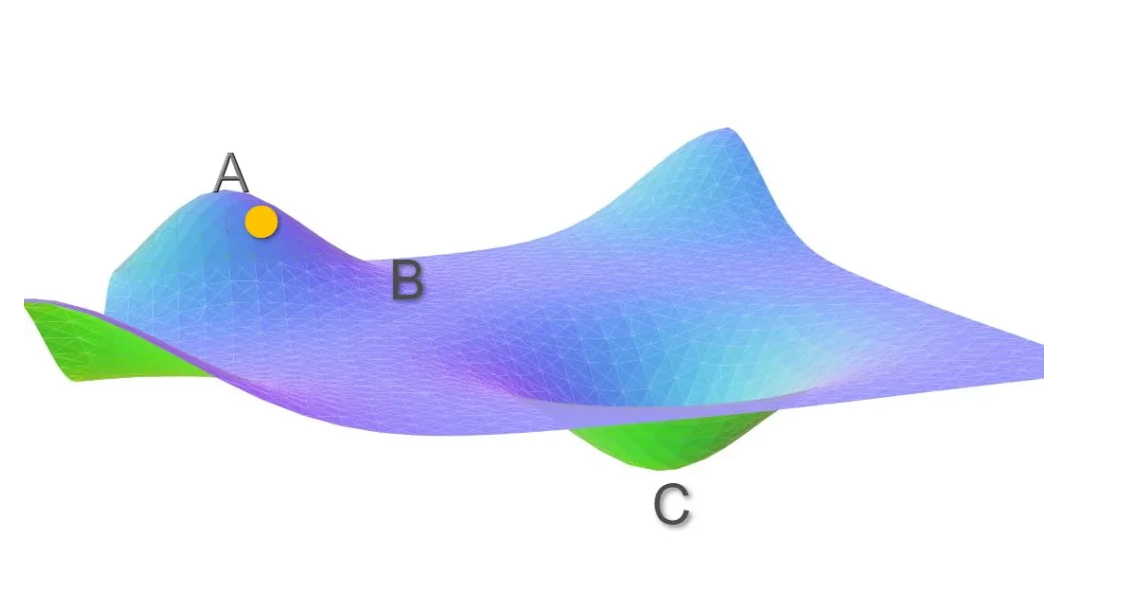
\includegraphics[scale=0.7]{images/momentum.png}
\end{center}
Let’s assume the initial weights of the network under consideration correspond to point A. With gradient descent, the Loss function decreases rapidly along the slope AB as the gradient along this slope is high. But as soon as it reaches point B the gradient becomes very low. The weight updates around B is very small. Even after many iterations, the cost moves very slowly before getting stuck at a point where the gradient eventually becomes zero.\newline\newline
Now, Imagine you have a ball rolling from point A. The ball starts rolling down slowly and gathers some momentum across the slope AB. When the ball reaches point B, it has accumulated enough momentum to push itself across the plateau region B and finally following slope BC to land at the global minima C.\newline\newline
The momentum algorithm accumulates an exponentially decaying moving average of past gradients and continues to move in their direction:
\[\textbf{v}(t) = \alpha\textbf{v}(t - 1) - \epsilon\sigma(t)\]
\[\theta = \theta + \textbf{v(t)}\]
where:
\begin{itemize}
    \item $\textbf{v}(t)$ is called \textbf{velocity} vector and determines the new weight update done at iteration $t$.
    
    \item $\alpha$ is a hyperparameter between 0 and 1 which determines how quickly the contributions of previous gradients exponentially decay.

    \item $\sigma(t) = \nabla_\theta \left(\frac{1}{m}\sum_{i=1}^m L(f(\textbf{x}^{(i)}; \theta), \textbf{y}^{(i)})\right)$ is the gradient at iteration $t$.
\end{itemize}
Assume that $\textbf{v}(0) = 0$:
\begin{equation}
    \begin{split}
        \textbf{v}(0) & = 0 \\
        \textbf{v}(1) & = \alpha\textbf{v}(0) - \epsilon\sigma(1)\\
        \textbf{v}(1) & = -\epsilon\sigma(1) \\
        & \\
        \textbf{v}(2) & = \alpha\textbf{v}(1) - \epsilon\sigma(2)\\
        \textbf{v}(2) & = \alpha (-\epsilon\sigma(1)) -\epsilon\sigma(2)\\
        \textbf{v}(2) & = -\epsilon (\alpha\sigma(1) + \sigma(2))\\
        & \\
        \textbf{v}(3) & = \alpha\textbf{v}(2) - \epsilon\sigma(3)\\
        \textbf{v}(3) & = -\epsilon(\alpha^2\sigma(1) + \alpha\sigma(2) + \sigma(3))
    \end{split}
\end{equation}
Let's \textit{ignore} the learning rate $\epsilon$ and focus on $\alpha$:
\begin{itemize}
    \item with $\alpha = 0.1$, at the third iteration the gradient at $t = 3$ will contribute 100\% of its value, the gradient at $t=2$ will contribute 10\% of its value, and gradient at t=1 will only contribute 1\% of its value (the contribution from earlier gradients decreases rapidly).

    \item with $\alpha = 0.9$, at the third iteration the gradient at $t = 3$ will contribute 100\% of its value, $t=2$ will contribute 90\% of its value, and gradient at $t=1$ will contribute 81\% of its value.
\end{itemize}
From above, we can deduce that the larger $\alpha$, the more previous gradients affect the current direction. Note that the actual contribution of each gradient in the weight update will be further subjected to the learning rate.\newline\newline
Common values of $\alpha$ used in practice include $.5$, $.9$, and $.99$. Like the learning rate, $\alpha$ may also be adapted over time.
\begin{center}
    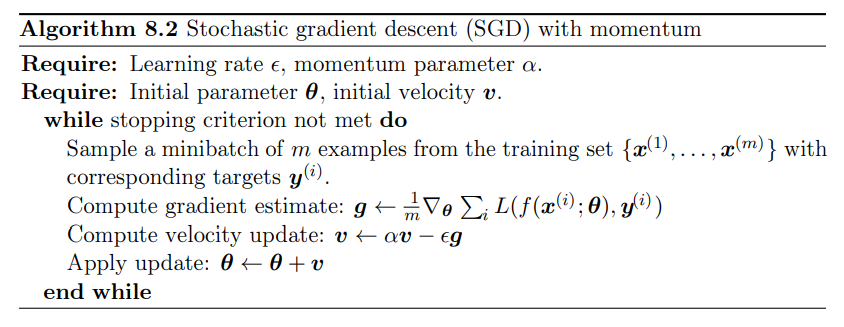
\includegraphics[]{images/Momentum alg.png}
\end{center}
When all the past gradients have the same sign we will take large steps while updating the weights. Even if the learning rate is low, all the gradients along the curve will have the same direction, thus increasing the momentum and accelerating the descent.\newline\newline
Another problem that momentum solves is poor conditioning of the Hessian matrix.
\begin{center}
    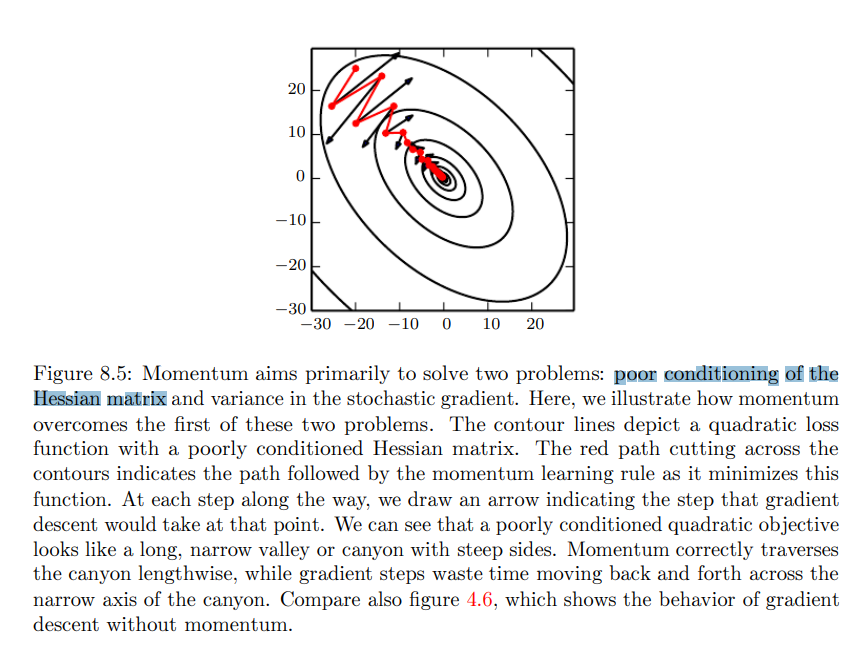
\includegraphics[]{images/poor cond. momentum.png}
\end{center}
In fact, the gradient in one direction is decreased if the gradient direction repeatedly changes as the terms in the sum cancel out.\newline\newline
The overall effect is a smoother trajectory and reduced oscillatory
behavior in valleys
\subsection{Nesterov momentum}
Nesterov momentum introduces a variant of the momentum algorithm. The difference between Nesterov momentum and standard momentum is where the gradient is evaluated. With Nesterov momentum the gradient is evaluated after the current velocity is applied.
\begin{center}
    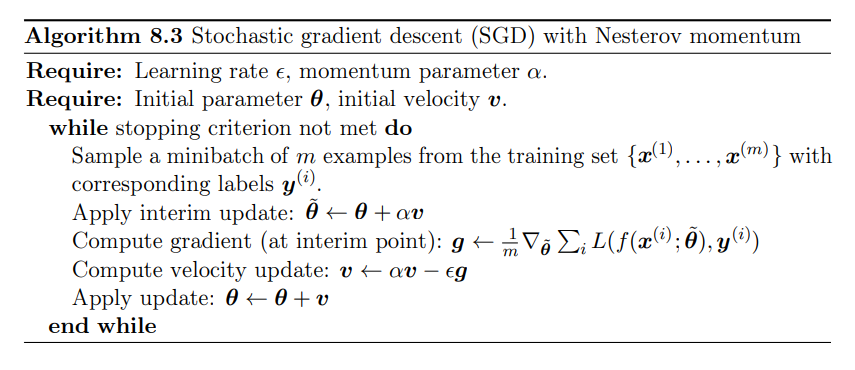
\includegraphics[]{images/nesterov momentum.png}
\end{center}

\section{Parameter initialization}
Deep Learning training algorithms are iterative and depends on initialization. The initial point can determine whether the algorithm converges at all, with some initial points being so unstable that the algorithm encounters numerical difficulties and fails altogether. The use of an optimization algorithm such as stochastic gradient descent that makes small incremental changes to the weights and tends to halt in areas that are nearer to the initial parameters, expresses a
prior that the final parameters should be close to the initial parameters.\newline\newline
Modern initialization strategies are simple and heuristic. Designing improved
initialization strategies is a difficult task because neural network optimization is not yet well understood. Perhaps the only property known with complete certainty is that the initial parameters need to “break symmetry” between different units.\newline\newline
If all the weights in a layer are initialized to the same value, each neuron will compute exactly the same function. The gradient will also be the same, so the weights associated to each neuron will evolve having exactly the same values. In other words, the layer will be equivalent to a layer with only one neuron.\newline\newline
We almost always initialize all the weights in the model to values drawn randomly from a Gaussian or uniform distribution. The choice of Gaussian or uniform distribution does not seem to matter very much, but has not been exhaustively studied. The scale of the initial distribution, however, does have a large effect on both the outcome of the optimization procedure and on the ability of the network to generalize.\newline\newline
Larger initial weights will yield a stronger symmetry breaking effect, helping to avoid redundant units. Initial weights that are
too large may, however, result in exploding values during forward propagation or back-propagation. Large weights may also result in extreme values that cause the activation function to saturate, causing complete loss of gradient through saturated units.\newline\newline
The perspectives of regularization and optimization can give very different insights into how we should initialize a network. The optimization perspective suggests that the weights should be large enough to propagate information successfully, but some regularization concerns encourage making them smaller.\newline\newline
Some heuristics are available for choosing the initial scale of the weights. One heuristic is to initialize the weights of a fully connected layer with $m$ inputs and $n$ outputs by sampling each weight from:
\[U(-\frac{1}{\sqrt{m}}, \frac{1}{\sqrt{m}})\]
while others suggest using the normalized initialization:
\[W_{i,j} \sim U\left( -\sqrt{\frac{6}{m + n}}, \sqrt{\frac{6}{m + n}}   \right)\]
Typically, we set the biases for each unit to heuristically chosen constants, and initialize only the weights randomly.
\subsection{Pre-training}
We can use pre-trained models as starting points for our models. For example:
\begin{itemize}
    \item Unsupervised pre-training: Train an unsupervised model on the training data, use the resulting model as initialization.

    \item Supervised pre-training (transfer learning): Initialize the weights with a model trained on a related task (Especially effective with CNNs).
\end{itemize}

\section{Adaptive learning rates}
Gradient descent with a fixed step size has an undesirable property: it makes:
\begin{itemize}
    \item large adjustments to parameters associated with large gradients (where perhaps we should be more cautious).

    \item small adjustments to parameters associated with small gradients (where perhaps we should explore further).
\end{itemize}
When the gradient of the loss surface is much steeper in one direction than another, it is difficult to choose a learning rate that makes good progress in both directions and is stable. It can make sense to use a separate learning rate for each parameter, and automatically adapt these learning rates throughout the course of learning.
\newline\newline
The delta-bar-delta algorithm is an early heuristic approach
to adapting individual learning rates for model parameters during training. The approach is based on a simple idea: if the partial derivative of the loss, with respect to a given model parameter, remains the same sign, then the learning rate should increase. If the partial derivative with respect to that parameter changes sign, then the learning rate should decrease. Of course, this kind of rule can only be applied to full batch optimization.\newline\newline
More recently, a number of incremental (or mini-batch-based) methods have been introduced that adapt the learning rates of model parameters.

\subsection{AdaGrad}
The AdaGrad algorithm individually adapts the learning rates of all model parameters by scaling them inversely proportional to the square root of the sum of all of the historical squared values of the gradients. Parameters with large partial derivatives will se a rapid decrease in their learning rate.\newline\newline
In the context of convex optimization, the AdaGrad algorithm enjoys some desirable theoretical properties. However, empirically it has been found that—for training deep neural network models—the accumulation of squared gradients from
the beginning of training can result in a premature and excessive decrease in the effective learning rate.
\begin{center}
    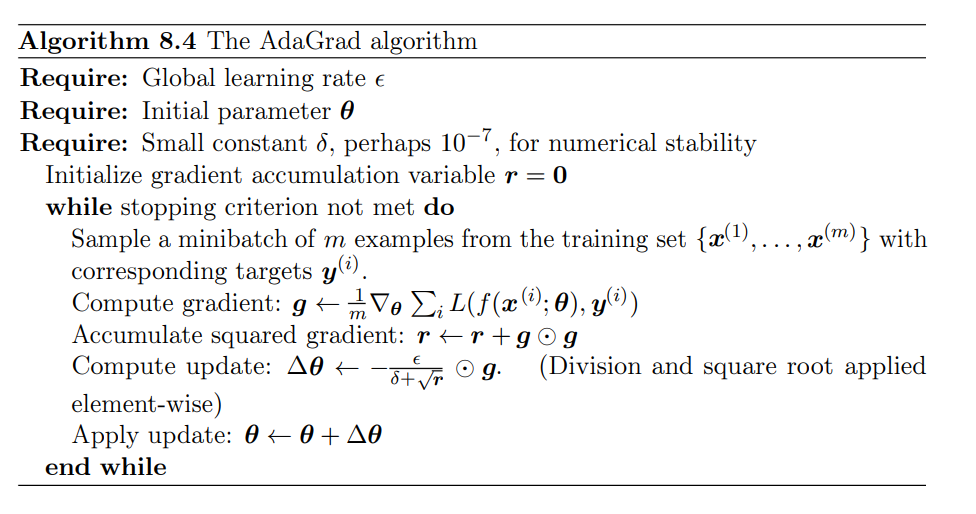
\includegraphics[scale=0.7]{images/AdaGrad.png}
\end{center}

\subsection{RMSprop}
The RMSProp algorithm modifies AdaGrad to perform better in the non-convex setting by changing the gradient accumulation into an exponentially weighted moving average.\newline\newline
Compared to AdaGrad, the use of the moving average introduces a new hyperparameter, $\rho$, that controls the length scale of the moving average. Empirically, RMSProp has been shown to be an effective and practical optimization algorithm for deep neural networks.
\begin{center}
    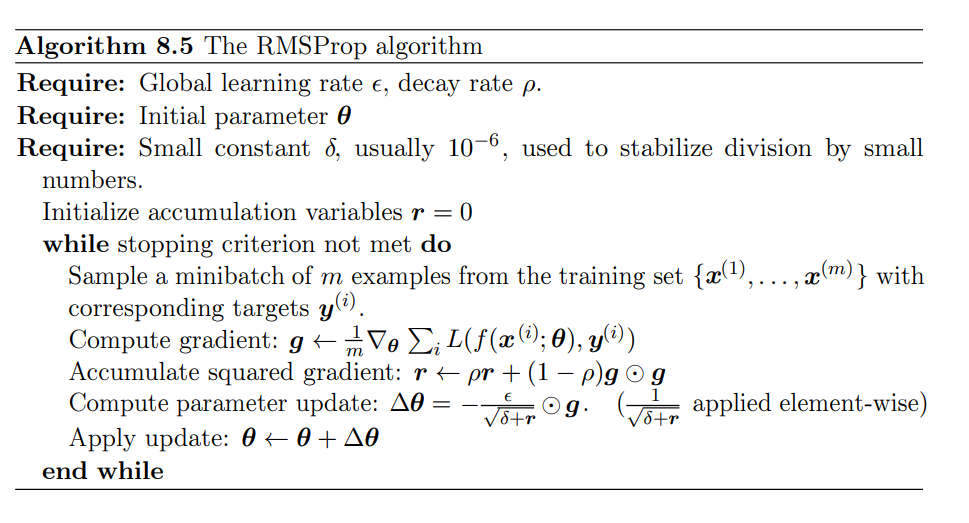
\includegraphics[scale=0.7]{images/RMSProp.png}
\end{center}

\subsection{Adam}
Adam includes bias corrections to the estimates of both the first-order moments (the momentum term) and the (uncentered) second-order moments to account for their initialization at the origin.\newline\newline
Adam is generally regarded as being fairly robust to the choice
of hyperparameters, though the learning rate sometimes needs to be changed from the suggested default.

\section{Second order methods}
In contrast to first-order methods, second-order methods make use of second derivatives to improve optimization. The most widely used second-order method is \textbf{Newton’s method}. Newton’s method is an optimization scheme based on using a second-order Taylor series expansion to approximate $J(\theta)$ near some point $\theta_0$, ignoring derivatives of higher order\footnote{the objective function $J(\theta)$ is the empirical risk}:
\[J(\theta) \approx J(\theta_0) + (\theta - \theta_0)^T \nabla_\theta J(\theta_0) + \frac{1}{2} (\theta - \theta_0)^T \textbf{H}(\theta - \theta_0)\]
where \textbf{H} is the Hessian of $J$ with respect to $\theta$ evaluated at $\theta_0$. If we then solve for the critical point of this function, we obtain the Newton parameter update rule:
\[\theta^* = \theta_0 - \textbf{H}^{-1}\nabla_\theta J(\theta_0)\]
If the function is quadratic, Newton’s method finds directly the minimum, if not, it can be applied iteratively. However, Computing $\textbf{H}$ and $\textbf{H}^{-1}$, is unfeasible for medium-sized networks.\newline\newline
Conjugate gradients is a method to efficiently avoid the calculation of the inverse Hessian by iteratively descending \textbf{conjugate directions}. . The inspiration for this approach follows from a careful study of the weakness of the method of steepest descent, where line searches are applied iteratively in the direction associated with the gradient.\newline\newline
In the method of conjugate gradients, we seek to find a search direction that is conjugate to the previous line search direction, i.e. it will not undo progress made in that direction. At training iteration $t$, the next search direction $\textbf{d}_t$ takes the form:
\[\textbf{d}_t = \nabla_\theta J(\theta) + \beta_t \textbf{d}_{t-1}\]
where $\beta_t$ is a coefficient whose magnitude controls how much of the direction, $\textbf{d}_{t-1}$, we should add back to the current search direction.\newline\newline
Two directions, $\textbf{d}_t$ and $\textbf{d}_{t-1}$, are defined as conjugate if $\textbf{d}_t^T \textbf{H}\textbf{d}_{t-1} = 0$, where $\textbf{H}$ is the Hessian matrix. Fortunately, we can compute the correct $\beta_t$ without computing $\textbf{H}$.\newline\newline
For quadratic surfaces in $k$ dimensions, conjugate gradients method requires at most $k$ steps to achieve the minimum (it can be adapted for non-quadratic surfaces).


\section{Batch normalization}
LeCun et al. (1998) showed that normalizing the inputs speeds
up training. Loffe and Szegedy (2015) proposed Batch Normalization to normalize hidden (pre-)activations:
\begin{itemize}
    \item each unit’s pre-activation is normalized (mean subtraction, standard deviation division).

    \item during training, mean and standard deviation is computed for each mini-batch.

    \item backpropagation takes into account the normalization.

    \item at test time, the global mean and global standard deviation is used. It requires a final phase where, from the first to the last hidden layer:
    \begin{itemize}
        \item propagate all training data to that layer.
        \item compute and store the global mean and global standard deviation for each unit.
    \end{itemize}

\end{itemize}
Normalize the pre-activation can help to keep the pre-activation in a non-saturating regime. 


\chapter{Lec 13 - Resolution for First Order Logic}

\section{Resolution}
The last of our three families of logical systems is based on \textbf{resolution}. In resolution for first order logic two clauses, which are assumed to be standardized apart so
that they share no variables, can be resolved if they contain complementary literals. Propositional literals are complementary if one is the negation of the other; first-order literals are complementary if one unifies with the negation of the other. Thus, we have
\begin{center}
    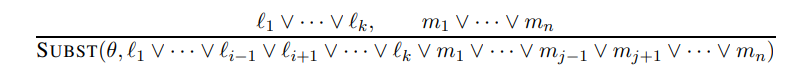
\includegraphics[]{images/resolution-fol.png}
\end{center}
where $UNIFY(l_i,\neg{m_j} ) = \theta$. For example, we can resolve the two clauses
\[[Animal(F(x)) \lor Loves(G(x), x)]\,\, \text{and} \,\,[\neg Loves(u, v) \lor \neg Kills(u, v)]\]
by eliminating the complementary literals $Loves(G(x), x)$ and $\neg Loves(u, v)$, with unifier $\theta = \{u/G(x), v/x\}$, to produce the \textbf{resolvent} clause
\[[Animal(F(x)) \lor \neg Kills(G(x), x)] .
\]
Then, the resolution steps can be applied to $CNF(KB \land \neg \alpha)$ as we did for propositional logic.

\section{Conversion to CNF}
As in the propositional case, first-order resolution requires that sentences be in \textbf{conjunctive
normal form} (CNF), that is, a conjunction of clauses, where each clause is a disjunction of literals. Literals can contain variables, which are assumed to be universally quantified. Every sentence of first-order logic can be converted into an inferentially equivalent CNF
sentence.\\\\
We illustrate the procedure by translating the sentence “Everyone who loves all animals is loved by someone,” or
\[\forall x \, [\forall y \, Animal(y) \Rightarrow Loves(x, y)] \Rightarrow [\exists y \, Loves(y, x)].\]
The steps are as follows:
\begin{itemize}
    \item \textbf{Eliminate implications:}
    \[\forall x \, [\neg \forall y \, \neg Animal(y) \lor Loves(x, y)] \lor [\exists y \, Loves(y, x)] .\]

    \item \textbf{Move} $\neg$ \textbf{inwards}: In addition to the usual rules for negated connectives, we need rules for negated quantifiers. Thus, we have
    \[\begin{split}
        & \neg \forall x \, p \,\, \text{becomes} \,\, \exists x \, \neg p\\
        & \neg \exists x \, p \,\, \text{becomes} \,\, \forall x \, \neg p .
    \end{split}\]
    Our sentence goes through the following transformations:
    \[\begin{split}
        & \forall x \, [\exists y \, \neg(\neg Animal(y) \lor Loves(x, y))] \lor [\exists y \, Loves(y, x)].\\
        & \forall x \,[\exists y \, \neg \neg Animal(y) \land \neg Loves(x, y)] \lor [\exists y \, Loves(y, x)].\\
        & \forall x \,[\exists y \, Animal(y) \land \neg Loves(x, y)] \lor [\exists y \, Loves(y, x)]
    \end{split}
    \]

    \item \textbf{Standardize variables}: each quantifier should use a different one:
    \[\forall x \,[\exists y \, Animal(y) \land \neg Loves(x, y)] \lor [\exists z \, Loves(z, x)] .\]

    \item \textbf{Skolemize:} \textbf{Skolemization} is the process of removing existential quantifiers by elimination. In the simple case, it is just like the Existential Instantiation rule seen previously: translate $\exists x \, P(x)$ into $P(A)$, where $A$ is a new constant. However, we can’t apply Existential Instantiation to our sentence above. If we blindly apply the rule to the two matching parts we get
    \[\forall x \, [Animal(A) \land \neg Loves(x, A)] \lor Loves(B,x),\]
    which has the wrong meaning entirely: it says that everyone either fails to love a particular animal $A$ or is loved by some particular entity $B$. Thus, we want the Skolem entities to depend on $x$ and $z$:
    \[\forall x \, [Animal(F(x)) \land \neg Loves(x, F(x))] \lor Loves(G(z), x) .\]
    Here $F$ and $G$ are \textbf{Skolem functions}.  The general rule is that the arguments of the Skolem function are all the universally quantified variables in whose scope the existential quantifier appears.

    \item \textbf{Drop universal quantifiers:}  At this point, all remaining variables must be universally quantified. Moreover, the sentence is equivalent to one in which all the universal quantifiers have been moved to the left. We can therefore drop the universal quantifiers:
    \[[Animal(F(x)) \land \neg Loves(x, F(x))] \lor Loves(G(z), x) .\]


    \item \textbf{Distribute} $\lor$ \textbf{over} $\land$:
    \[[Animal(F(x)) \lor Loves(G(z), x)] \land [\neg Loves(x, F(x)) \lor Loves(G(z), x)].\]
\end{itemize}
The sentence is now in CNF and consists of two clauses.

\section{Example proofs}
Resolution proves that $KB \vDash \alpha$ by proving $KB \land \neg \alpha$ unsatisfiable, that is, by deriving the empty clause. The algorithmic approach is identical to the propositional case. We give two example proofs. The first is the crime example presented in the previous sections. The sentences in CNF are:
\begin{center}
    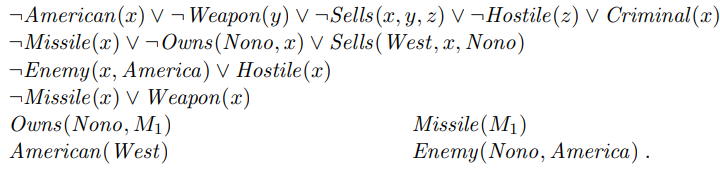
\includegraphics[]{images/crime-cnf.png}
    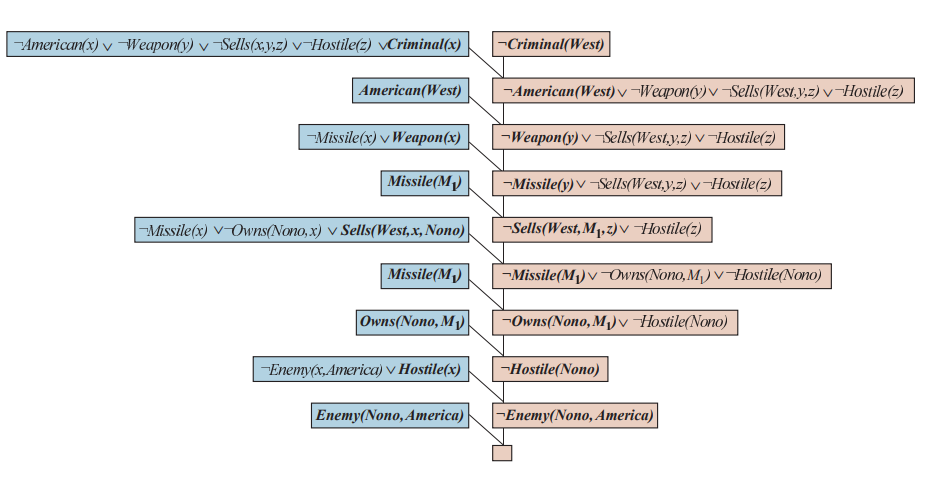
\includegraphics[]{images/resolution-crime-fol.png}
\end{center}
The resolution proof is shown in the figure above. Notice the structure: single “spine” beginning with the goal clause, resolving against clauses from the knowledge base until the empty clause is generated. This is characteristic
of resolution on Horn clause knowledge bases. In fact, the clauses along the main spine correspond exactly to the consecutive values of the goals variable in the backward-chaining algorithm.\\\\
Our second example makes use of Skolemization and involves clauses that are not definite clauses. This results in a somewhat more complex proof structure. In English, the problem is as follows:
\begin{center}
    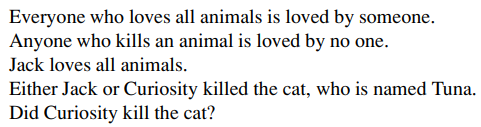
\includegraphics[]{images/resolution-fol-proof.png}
\end{center}
First, we express the original sentences, some background knowledge, and the negated goal G in first-order logic:
\begin{center}
    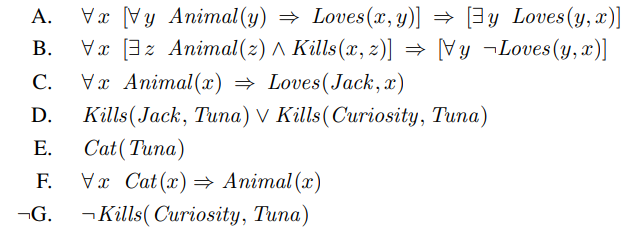
\includegraphics[]{images/kb-res-proof.png}
\end{center}
Now we apply the conversion procedure to convert each sentence to CNF:
\begin{center}
    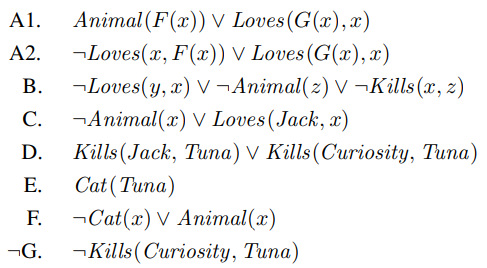
\includegraphics[]{images/kb-cnf-re-prrof.png}
\end{center}
The resolution proof that Curiosity killed the cat is given in the figure below:
\begin{center}
    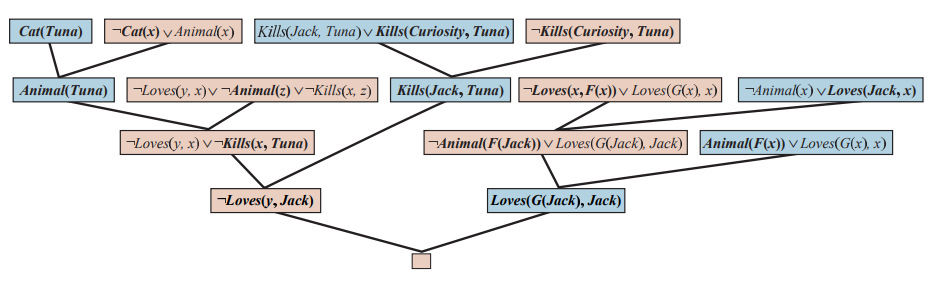
\includegraphics[]{images/res-proof-tree.png}
\end{center}
The proof answers the question “Did Curiosity kill the cat?” but often we want to pose more general questions, such as “Who killed the cat?”. Then, the goal is $\exists w \, Kills(w, Tuna)$, which, when negated, becomes $\neg Kills(w, Tuna)$ in CNF. Repeating the proof with the new negated goal, we obtain a similar proof tree, but with the substitution {w/Curiosity} in one of the steps. Unfortunately, resolution can produce \textbf{nonconstructive proofs} for existential goals. For example, $\neg Kills(w, Tuna)$ resolves with $Kills(Jack, Tuna) \lor Kills(Curiosity, Tuna)$ to give $Kills(Jack, Tuna)$, which resolves again with $\neg Kills(w, Tuna)$ to yield the empty clause. Notice that $w$ has two different bindings in this proof; resolution is telling us that, yes, someone killed Tuna, either Jack or Curiosity. This is no great surprise!
\begin{center}
    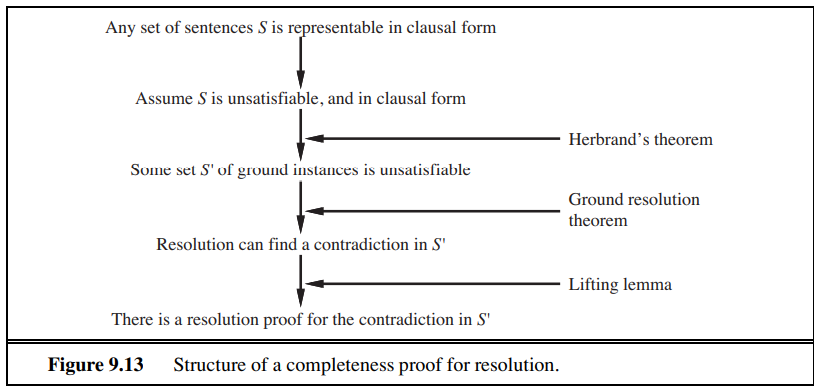
\includegraphics[]{images/res-completeness-fol.png}
\end{center}

\section{Resolution strategies}
We know that repeated applications of the resolution inference rule will eventually find a proof if one exists. In this subsection, we examine strategies that help find proofs efficiently.
\begin{itemize}
    \item \textbf{Unit preference/clause}: prefers to do resolutions where one of the sentences is a single literal.  The idea behind the strategy is that we are trying to produce an empty clause, so it might be a good idea to prefer inferences that produce shorter clauses.

    \item \textbf{Unit resolution:} is a restricted form of resolution in which every resolution step \textbf{must} involve a unit clause. Unit resolution is incomplete in general, but complete for Horn clauses. Unit resolution proofs on Horn clauses resemble forward chaining.

    \item \textbf{Set of support:} every resolution step involve at least one element of a special set of clauses (the set of support); the resolvent is then added into the set of support. Incomplete if the wrong set of support is chosen.

    \item \textbf{Input resolution:} In this strategy, every resolution combines one of the input sentences (from the KB or the query) with some other sentence. Complete for knowledge bases that are in Horn form, but incomplete in the general case. Input resolution has the characteristic shape of a single “spine” with single sentences combining onto the spine. The \textbf{linear resolution} strategy is a slight generalization that allows $P$ and $Q$ to be resolved together either if $P$ is in the original KB or if $P$ is an ancestor of $Q$ in the proof tree. Linear resolution is complete.

    \item \textbf{Subsumption:} eliminates all sentences that are subsumed by (that is, more specific than) an existing sentence in the KB. For example, if $P(x)$ is in the KB, then there is no sense in adding $P(A)$ and even less sense in adding $P(A) \lor Q(B)$. Subsumption helps keep the KB small and thus helps keep the search space small.

\end{itemize}

\chapter{Lec 14 - Higher-order functions for trees III}

\section{Trees type definition}
Until now we used binary trees that support data only in the leaves. Let's change the type definition in order to support information attached to nodes. We can do this in many different ways:
\begin{lstlisting}[style = FSharpStyle]
    type 'a tree =
        | Node of 'a * 'a tree * 'a tree
        | Leaf of 'a
\end{lstlisting}
In this case, a node is composed by an element of type 'a (which is the information attached to it) and the two sub-trees. However, with this definition we wouldn't be able to represent dead branches. In fact, each node must always have two sub-trees that can be either another node or a leaf.
\begin{lstlisting}[style = FSharpStyle]
    type 'a tree =
        | Node of 'a * 'a tree * 'a tree
        | Leaf of 'a option
\end{lstlisting}
With this implementation we can represent a dead branch defining a Leaf of None, but we could even define nodes with two empty leaves. So, this definition allows the programmer to write things that are not in their most simplified form.\newline\newline
In order to prevent this, we can do the following:
\begin{lstlisting}[style = FSharpStyle]
    type 'a tree =
        | Node of 'a * 'a tree option * 'a tree option
\end{lstlisting}
Now the \textbf{Node} data-constructor is a triple composed by:
\begin{itemize}
    \item An element of type 'a (information in the node)
    \item Two 'a tree option elements which represent the left and right sub-trees
\end{itemize}
When both the sub-trees are None, we are representing a leaf.\newline\newline
Let's write in F\# the following tree using this definition:\newline
\begin{tikzpicture}
    \Tree
    [.5  
        [.6
            \edge[]; {1}
            \edge[]; {2}
        ]
        [.7
            \edge[]; {3}
            \edge[blank]; \node[blank]{};
        ]
    ]
\end{tikzpicture}\newline
\begin{lstlisting}[style = FSharpStyle]
    let Leaf x = Some(Node(x, None, None))
    let tree = Node(5,
                Some(Node(6, Leaf 1, Leaf 2)),
                Some(Node(7, Leaf 3, None)))
\end{lstlisting}
Note that \textbf{Leaf x} is a function, not a data-constructor. It is just a shorter way to define leaves. The difference between functions and data-constructors is that functions can be used to \textbf{create}, but not for deconstructing (they can't be used to pattern-match).\newline\newline
We can write trees even in a shorter form by defining the following function:
\begin{lstlisting}[style = FSharpStyle]
    let SNode (x, t1, t2) = Some (Node (x, t1, t2))
    let tree = Node (5, 
               SNode (6, Leaf 1, Leaf 2), 
               SNode (7, Leaf 3, None)
               )
\end{lstlisting}
How can we pattern-match this type definition ? We have to specify all possible combinations of node types.
\begin{lstlisting}[style = FSharpStyle]
    let rec pretty_tree t = 
        match t with
        | Node(x, None, None) -> sprintf "(. %O .)" x
        | Node(x, Some l, Some r) -> sprintf "(%s %O %s)" (pretty_tree l) x (pretty_tree r)
        | Node(x, Some l, None) -> sprintf "(%s %O %s)" (pretty_tree l) x "."
        | Node (x, None, Some r) -> sprintf "(%s %O %s)" "." x (pretty_tree r)
        
    let st = pretty_tree tree

    // val st : string = "(((. 1 .) 6 (. 2 .)) 5 ((. 3 .) 7 .))"
\end{lstlisting}
The function above is a \textbf{pretty\_print} function for trees, which is a function that produces a string that represents the given tree. Instead of specify all the possibilities in the pattern-match, we can simplify things by defining an additional function. 
\begin{lstlisting}[style = FSharpStyle]
    let pretty_opt f o = 
        match o with 
        | None -> "."
        | Some x -> f x

    let rec pretty_tree t =
        match t with
        | Node (x, lo, ro) -> 
            let l = pretty_opt pretty_tree lo
            let r = pretty_opt pretty_tree ro
            sprintf "(%s %O %s)"  l x r
    
    let st = pretty_tree tree

    // val st : string = "(((. 1 .) 6 (. 2 .)) 5 ((. 3 .) 7 .))"
\end{lstlisting}
\section{Record types}
In F\# we can define the so called \textbf{record types} using the following syntax:
\begin{lstlisting}[style = FSharpStyle]
    type 'a tree = {data : 'a;
                     left : 'a tree option;
                     right : 'a tree option}
\end{lstlisting}
Records are series of \textit{Label : type} separated by a semicolon.


\chapter{Lec 15 - Sequence Modeling}

\section{Learning in Sequential Domains}
Why learning in sequential domains is different than static domains ? Because successive points in sequential data are \textbf{strongly correlated}. Machine learning models and algorithms for sequence learning have to consider that data points are not independent, deal with sequential distortions and/or variations (e.g. In speech, variations in speaking rate) and make use of \textbf{contextual information}.
\newline\newline
With static data we usually learn:
\[P(\textbf{o}|\textbf{x})\]
where $\textbf{x}$ is a fixed-size tuple of predictive attributes and $\textbf{o}$ is a classification/regression task.\newline\newline
With \textbf{sequential data}, instead, $\textbf{x}$ is a \textbf{sequence} $x^{(1)}, ..., x^{(t)}, ...$ where each $x^{(t)}$ has a static type. $\textbf{o}$ may be either static (e.g., sequence classification) or a sequence.\newline\newline
Using mathematical induction, a \textbf{sequence} is either an external vertex, or an ordered pair $(t, h)$ where the head $h$ is a vertex and the tail $t$ is a sequence.

\subsection{Sequencial Transductions}
Sequence Transduction is a machine learning task that involves converting an input sequence into an output sequence, potentially of different lengths.\newline\newline
Let $X$ and $O$ be the \textbf{input} and \textbf{output} label spaces. We denote by $X^*$ the set of all sequences with labels in $X$. We can define a general transduction $T$ as a function
\[T : X^* \rightarrow O^*\]
\begin{itemize}
    \item $T(\cdot)$ has \textbf{finite memory} $k \in \mathbb{N}$ if $\forall \textbf{x} \in X^*$ and $\forall t$, $T(x^{(t)})$ only depends on $\{\textbf{x}^{(t)}, \textbf{x}^{(t-1)}, ..., \textbf{x}^{(t-k)}\}$ 

    \item $T(\cdot)$ is \textbf{algebraic} if it has 0 finite memory (i.e., no memory at all)

    \item A transduction $T(\cdot)$ is \textbf{causal} if the output at time $t$ does not depend on future inputs (at time $t + 1, t + 2,...$ )

\end{itemize}

\subsection{Learning Sequences}
Sequences have variable length but typical machine learning models
have a fixed number of inputs. In order to solve this problem we can:
\begin{itemize}
    \item Limit context to a \textbf{fixed-size window}.
    \item Use \textbf{recurrent} models.
    \item Use \textbf{transformers} for non-causal sequences (e.g. text).
\end{itemize}


\section{Recursive State Representation}
In order to represent a recursive state we can use the following equations:
\[\begin{split}
    h^{(t)} & = f(h^{(t-1)}, x^{(t)}, t)\\
    o^{(t)} & = g(h^{(t)}, x^{(t)}, t)
\end{split}\]
where $f$ is the \textit{state transition function} and $g$ is the \textit{output function}. 
\newline\newline
$h^{(t)}$ is called the state of the system and it's defined by a \textbf{recursive equation}. Indeed, the definition of $h$ at time $t$ refers back to the same definition at time $t - 1$. It contains information about the whole past sequence. For a finite number of time steps $\tau$, the graph can be unfolded by applying the definition $\tau - 1$ times. \textbf{Unfolding} the equation by repeatedly applying the definition yields an expression that does not involve recurrence. Such an expression can now be represented by a traditional directed acyclic computational graph.
\begin{center}
    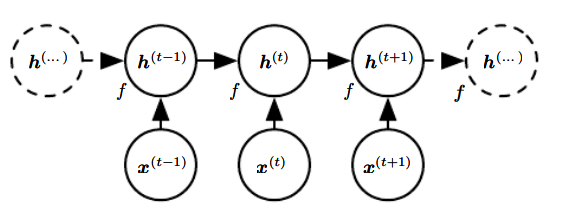
\includegraphics[]{images/recurrent-graph.png}
\end{center}
The state transition function can be represented using the time shift operator $q^{-1}$:
\[q^{-1}h^{(t)} = h^{(t-1)}\]
\begin{center}
    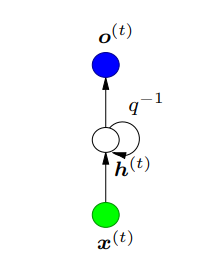
\includegraphics[]{images/time-shift-op.png}
\end{center}
The unfolding process thus introduces two major advantages:
\begin{enumerate}
    \item Regardless of the sequence length, the learned model always has the same input size, because it is specified in terms of transition from one state to another state, rather than specified in terms of a variable-length history of states.

    \item It is possible to use the same transition function $f$ with the same parameters at every time step.
\end{enumerate}
These two factors make it possible to learn a single model that operates on all time steps and all sequence lengths. Learning a single, shared model allows generalization to sequence lengths that did not appear in the training set, and allows the model to be estimated with far fewer training examples than would be required without parameter sharing.\newline\newline
Given a sequence $s \in X^{*}$ and a recursive transduction $T$, the \textit{encoding network} associated to $s$ and $T$ is formed by unrolling (time unfolding) the recursive network of $T$ through the input sequence $s$.
\begin{center}
    \includegraphics[]{images/encoding-network.png}
    \includegraphics[scale=0.7]{images/sequential--transduction.png}
\end{center}
$T$ is \textbf{stationary} if $f(\cdot)$ and $g(\cdot)$ do not depend on $t$\newline\newline
There are different ways in which we can implement $f(\cdot)$ and $g(\cdot)$. There are two general families of models:
\begin{itemize}
    \item Linear:
    \begin{itemize}
        \item Kalman Filter
        \item Hidden Markov Models
        \item Linear Dynamical Systems
        \item ...
    \end{itemize}
    \item Nonlinear
    \begin{itemize}
        \item Recurrent Neural Networks
        \item ...
    \end{itemize}
\end{itemize}

\section{Shallow Recurrent Neural Networks}
Armed with the graph unrolling and parameter sharing ideas, we can design a wide variety of recurrent neural networks. In general we have:
\[\begin{split}
    \textbf{h}^{(t)} & = f(\textbf{U}\textbf{x}^{(t)} + \textbf{W}\textbf{h}^{(t-1)} + \textbf{b})\\
    \textbf{o}^{(t)} & = g(\textbf{V}\textbf{h}^{(t)} + \textbf{c})
\end{split}\]
where $f()$ and $g()$ are non-linear functions (e.g. $tanh()$ and $softmax$), and $h^{(0)} = 0$ (or can be learned jointly with the other parameters). $\textbf{U}$ and $\textbf{W}$ are weight matrices which parametrize \textbf{input-to-hidden} connections and \textbf{hidden-to-hidden} recurrent connections respectively. \textbf{Hidden-to-output} connections are parametrized by the weight matrix $\textbf{V}$.\newline\newline
An example of RNN for IO-transduction with discrete outputs:
\[\begin{split}
    \textbf{h}^{(t)} & = tanh(\textbf{U}\textbf{x}^{(t)} + \textbf{W}\textbf{h}^{(t-1)} + \textbf{b})\\
    \textbf{o}^{(t)} & = \textbf{V}\textbf{h}^{(t)} + \textbf{c}\\
    \hat{\textbf{y}} & = softmax(\textbf{o}^{(t)})\\
    L & = \sum_t L^{(t)} = - \sum_t log\,p_{model}(\textbf{y}^{(t)} | \{\textbf{x}^{1}, ..., \textbf{x}^{(t)}\})
\end{split}\]
where:
\begin{itemize}
    \item $o^{(t)}$ is the unnormalized log probabilities a time $t$
    \item $\textbf{y}^{(t)}$ is the target vector a time $t$
    \item $p_{model}(\textbf{y}^{(t)} | \{\textbf{x}^{1}, ..., \textbf{x}^{(t)}\}$ is given by reading the entry for $\textbf{y}^{(t)}$ from the model’s output vector $\hat{\textbf{y}}^{(t)}$, that is, the loss $L$ \textbf{internally computes} $\hat{\textbf{y}}$.
    \item $L$ is the loss function
\end{itemize}
The corresponding computation graph is the following
\begin{center}
    \includegraphics[scale=0.8]{images/rnn-computational-graph.png}
\end{center}
Some examples of important design patterns for recurrent neural networks
include the following:
\begin{itemize}
    \item Recurrent networks that produce an output at each time step and have recurrent connections between hidden units (IO-transduction).

    \item Recurrent networks that produce an output at each time step and have recurrent connections only from the output at one time step to the hidden units at the next time step

    \item Recurrent networks with recurrent connections between hidden units, that read an entire sequence and then produce a single output (e.g. for classification).
\end{itemize}
There are a lot of possible additional architectural features, such as short-cut connections, higher-order states, feedback from output, teacher forcing, bidirectional RNN, etc\footnote{See slides for further information}. All these architectural features (and others...) are orthogonal, i.e. they can be combined together.


\subsection{Teacher Forcing}
The network with recurrent connections only from the output at one time step to the hidden units at the next time step is strictly less powerful because it lacks hidden-to-hidden recurrent connections. Therefore, it requires that the output units capture all of the information about the past that the network will use to predict the future. Because the output units are explicitly trained to match the training set targets, they are unlikely to capture the necessary information about the past history of the input.\newline\newline
For this reason, models that have recurrent connections from their outputs leading back into the model may be trained with \textbf{teacher forcing}. Teacher forcing is a procedure in which during training the model receives the ground truth output $\textbf{y}^{(t)}$ as input at time $t + 1$. When the model is deployed, the true output is generally not known. In this case, we approximate the correct output $\textbf{y}^{(t)}$ with the model’s output $\textbf{o}^{(t)}$, and feed the output back into the model.
\[\begin{split}
    \textbf{h}^{(t)} & = tanh(\textbf{U}\textbf{x}^{(t)} + \textbf{W}\textbf{y}^{(t-1)} + \textbf{b})\\
    \textbf{o}^{(t)} & = \textbf{V}\textbf{h}^{(t)} + \textbf{c}\\
    \hat{\textbf{y}} & = softmax(\textbf{o}^{(t)})\\
    L & = - \sum_t log\,p_{model}(\textbf{y}^{(t)} | \textbf{y}^{(1)}, ..., \textbf{y}^{(t-1)}, \textbf{x}^{(1)}, ..., \textbf{x}^{(t)})
\end{split}\]
\begin{center}
    \includegraphics[]{images/teacher-forcing.png}
\end{center}
The advantage of eliminating hidden-to-hidden recurrence is that, for any loss function based on comparing the prediction at time $t$ to the training target at time $t$, all the time steps are decoupled. Training can thus be parallelized, with the gradient for each step $t$ computed in isolation.

\subsection{Bidirectional RNNs}
in many applications we want to output a prediction of $\textbf{y}^{(t)}$ which may depend on the whole input sequence. For example, if there
are two interpretations of the current word that are both plausible, we may have to look far into the future (and the past) to disambiguate them. Bidirectional recurrent neural networks (or bidirectional RNNs) were invented to address that need.\newline\newline
As the name suggests, bidirectional RNNs combine an RNN that moves forward
through time, beginning from the start of the sequence, with another RNN that moves backward through time, beginning from the end of the sequence.
\begin{center}
    \includegraphics[scale=0.9]{images/bidirectional-rnn.png}
\end{center}

\subsection{1 to \textit{n} transduction}
Previously, we have discussed RNNs that take a sequence of vectors $\textbf{x}^{(t)}$ for $t = 1, ..., \tau$ as input. Another option is to take only a single vector $\textbf{x}$ as input. When $\textbf{x}$ is a fixed-size vector, we can simply make it an extra input of the RNN
that generates the $\textbf{y}$ sequence.  The interaction between the input $\textbf{x}$ and each hidden unit vector $\textbf{h}^{(t)}$ is parametrized by a newly introduced weight matrix $\textbf{R}$.
\begin{center}
    \includegraphics[scale=0.8]{images/1-to-n transduction.png}
\end{center}
Each element $\textbf{y}^{(t)}$ of the observed output sequence serves both as input (for the current hidden unit at time $t$) and, during training, as target (for the previous output unit at time $t-1$).\newline\newline
This RNN is appropriate for tasks such as image captioning, where a single image is used as input to a model that then produces a sequence of words describing the image.

\subsection{Encoder-Decoder Sequence-to-Sequence Architectures}
Here we discuss how an RNN can be trained to map an input sequence to an output sequence which is not necessarily of the same length. This comes up in many applications, such as speech recognition, machine translation, etc.\newline\newline
An encoder-decoder RNN architecture is is composed of an encoder RNN that reads the input sequence and a decoder RNN that generates the output sequence. The final hidden state of the encoder RNN is used to compute a generally fixed-size context variable $C$ which represents a semantic summary of the input sequence and is given as input to the decoder RNN.
\begin{center}
    \includegraphics[]{images/encoder-decoder rnn.png}
\end{center}
If the context $C$ is a vector, then the decoder RNN is simply a vector-to-sequence RNN.


\chapter{Lec 16 - Graph Neural Networks}

\section{Introduction}
Traditional ML approaches have been developed assuming data to be encoded into feature vectors; however, many important real-world applications generate data that are naturally represented by more complex structures, such as graphs. Graphs are particularly suited to
represent the relations (arcs) between the components (nodes) constituting an entity. For instance, in social network data, single data “points” (i.e., users) are closely inter-related.\newline\newline
A graph $G = (V, E)$ can be represented using the so called \textbf{adjacency matrix}. A $n \times n$ matrix $A$ such that $A[i,j] = 1$ if $edge(i,j) \in E$, 0 otherwise.\newline\newline
    \textbf{Example:}\newline\newline
    \begin{center}
        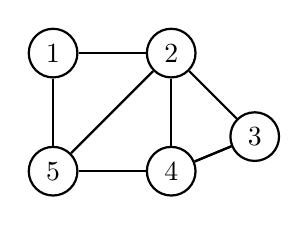
\begin{tikzpicture}[node distance={15mm}, thick, main/.style = {draw, circle}] 
            \node[main] (1) {$1$}; 
            \node[main] (2) [right of=1] {$2$}; 
            \node[main] (3) [below right of=2] {$3$}; 
            \node[main] (4) [below of=2] {$4$}; 
            \node[main] (5) [below of=1] {$5$}; 
            \draw (1) -- (2); 
            \draw (1) -- (5); 
            \draw (2) -- (5);
            \draw (2) -- (4);
            \draw (5) -- (4);
            \draw (3) -- (4); 
            \draw (5) -- (4);
            \draw (4) -- (3);
            \draw (2) -- (3);
        \end{tikzpicture}
    \end{center}
    The Adjacency matrix of the graph above is the following:
    \[\begin{bmatrix}
        0 & 1 & 0 & 0 & 1 \\
        1 & 0 & 1 & 1 & 1 \\
        0 & 1 & 0 & 1 & 0 \\
        0 & 1 & 1 & 0 & 1 \\
        1 & 1 & 0 & 1 & 0
    \end{bmatrix}\]
In undirected graphs this matrix is \textbf{symmetric}, while in directed graphs it is \textbf{asymmetric}. In case of a weighted graph, each cell of the matrix has either the value of the edge weight $w$ or $-$. Each node and edge is represented by a feature vector:
\begin{center}
    \includegraphics[scale=0.5]{images/graphs.png}
\end{center}
The position $(m,n)$, of the adjacency matrix contains the number of walks of length one from node $m$ to node $n$. Position $(m,n)$ of the \textbf{squared} adjacency matrix $A^2$ contains the number of walks of length two from node $m$ to node $n$.\newline\newline
The main problem settings that can arise when dealing with structured data are the following:
\begin{itemize}
    \item Predictions over \textbf{nodes} in a network: In this setting, the dataset is composed of a single (possibly disconnected) large graph. Each example is a node in the graph, and the learning tasks are defined as predictions over the nodes. Given an unseen node $u$, the task is to predict the correct target $y_u$. An example in this setting is the prediction of properties of a social network user based on his or her connections.

    \item Predictions over \textbf{graphs}: In this case, each example is composed of a whole graph, and the learning tasks are predictions of properties of the whole graphs. An example is the prediction of toxicity in humans of chemical compounds represented by their molecular graph.

    \item Link-prediction tasks: the model predicts whether or not there should be an edge between nodes. 
\end{itemize}

\section{Learning on graphs is difficult}
Let $\textbf{X}$ be the matrix in which the feature vectors of each node are stored. We can observe that node indexing in graphs is arbitrary. This means that, differently from images, permuting the node indices results in a permutation of the columns of $\textbf{X}$ and a permutation of both the rows and columns of $A$. However, the underlying graph is unchanged. This property is called Permutation Invariance. More formally, given a permutation matrix $\textbf{P}$, we get a different representation of the same graph:
\[\begin{split}
    \textbf{X}' & = \textbf{XP}\\
    \textbf{A}' & = \textbf{P}^T \textbf{AP}
\end{split}
\]
This property can give the intuition about why learning on graphs is difficult. In fact, determining if two graphs are equal (graphs isomorphism) is a problem for which are not known polynomial-time algorithms. Furthermore, sub-graph isomorphism, which is the problem of determining if a graph is a sub-graph of another graph, is NP-Complete. These problems affect machine learning because a model should be able to predict the same output for isomorphic graphs (which can be represented in different ways). Furthermore, the model we design should capture the similarity between two graphs (sub-graph isomorphism).\newline\newline
In general, the main problems we face when learning on graphs are the following:
\begin{enumerate}
    \item Same graph can be represented in different ways;
    \item How to recognize that a given graph $G_2$ is a sub-graph of $G_1$
    \item How to represent graphs of different sizes (i.e., different number of nodes) into fixed-size vectors without loosing expressiveness ?

    \item How to avoid explosion in the number of parameters with the size of the graphs?
    
\end{enumerate}
Problem 3 is commonly faced by using recursive models that exploit a
causal state space [Sperduti \& Starita., TNN 1997], while Problem 4  is commonly faced by exploiting shared parameters.\newline\newline
Regarding Problems 1 and 2, a sound and meaningful representation for graphs can be achieved by using a neural network with \textbf{convolution operator}, defined on graphs.

\section{Graph Neural Networks - General Idea}
A Graph Neural Network (GNN) receives in input a graph (adj. matrix and node representations. for simplicity) and passes it through a series of $k$ layers. Each layer computes a hidden representation for each node, with the last layer computing the final nodes' embeddings $\textbf{H}_k$. Similarly to CNNs, each node representation includes information about the node and its context within the graph.
\begin{itemize}
    \item For \textbf{node-level tasks}, the output is computed from $\textbf{H}_k$;

    \item For \textbf{graph-level tasks}, the nodes' embeddings are combined (e.g., by averaging), and the resulting vector is mapped via a linear transformation or neural network to a fixed-size vector from which the classification/regression task is performed.

    \item For \textbf{link-prediction tasks}, the embeddings of the two endpoint nodes must be mapped to a single number representing the probability that the edge is present (e.g. dot product of the nodes' embeddings and pass the result through a sigmoid function to create a probability).
 
\end{itemize}
\begin{center}
    \includegraphics[]{images/gnn.png}
\end{center}

\section{Graph Convolution}
The general idea of graph convolution starts from a parallel between graphs and images. GNNs implement convolution in a similar way how CNNs do, that is, learning the features by inspecting neighboring nodes. GNNs generalize the definition of convolution for non-regular structured data.

\subsection{NN4G by Micheli}
\textbf{NN4G} is an architecture based on a graph convolution that is defined as:
\begin{center}
    \includegraphics[scale=0.6]{images/nn4g.png}
\end{center}
where: 
\begin{itemize}
    \item $\sigma$ is a nonlinear activation function applied element-wise.
    \item $N(v)$ represent the neighborhood of node $v$.
    \item $\textbf{W}^i$ is a weights' matrix;
    \item $\textbf{x}_u$ is the feature vector of node $u$.
\end{itemize}
Actually, this is a simplified notation, since the original one uses skip connections (see GNN book chapter).
\begin{center}
    \includegraphics[]{images/nn4g-2.png}
\end{center}
Note that:
\begin{itemize}
    \item The first layer ($i = 1$), which has no previous layers, computes the nodes' representations only on the basis of each vertex feature vector.

    \item Each convolution performed on the $i$-th hidden units, with $i > 1$, takes as input the neighbors' representations of the previous layer. Basically, it merges the representations of each node with those of its neighbors:

    \item $X_1(g), X_2(g), X_3(g)$ are scalar values computed by aggregating the representations $\textbf{x}_i(g)$ for each unit $i$.
    In particular they are defined as:
    \[X_i(g) = \frac{1}{k}\sum_{v \in Vert(g)}x_i(v)\]
    if $k = 1$, this corresponds to a sum. Basically, we compute a representation per-graph per-layer. Then, this 3 representations are parametrized by the weights $w_1, w_2, w_3$ and used to compute the output for the whole graph (graph-level task).
\end{itemize}
The convolutional operation presented above can be defined in a compact way using matrix multiplications:
\begin{center}
    \includegraphics[scale=0.6]{images/matrix-gcn.png}
\end{center}
where $\textbf{A}$ is the adjacency matrix. Exploiting matrix multiplications makes the computation really fast. Furthermore, note that, as for images, the receptive field of the layers increases as we stack more layers.\newline\newline
Note also that, since with the convolution operator we are merging neighboring nodes' representations, isomorphic graphs in which the order of the nodes is changed will have the same nodes' representations.

\subsection{Graph Fourier Transform}
The operation described above is graph convolution, but how it is derived? Defining the formal convolution operator on graph is difficult.\newline\newline
Let $x: V \rightarrow \mathbb{R}$ be a signal on the nodes $V$ of the graph $G$, i.e., a function that associates a real value with each node of $V$. We can represent every signal as a vector $\textbf{x} \in \mathbb{R}^n$, which from now on we will refer to as signal. In order to set up a convolutional network on $G$, we need the notion of convolution between a signal $\textbf{x}$ and a filter signal $\textbf{f}$.\newline\newline
The key idea is to use a Fourier transform. In the frequency domain, thanks to the \textbf{Convolution Theorem}, the (undefined) convolution of two signals becomes the (well-defined) component-wise product of their transforms. So, if we knew how to compute the Fourier transform of a function defined on a graph, we could define the convolution operator.\newline\newline
The Convolution Theorem states that convolution in one domain (time, space) corresponds to pointwise multiplication in frequency domain.\newline\newline
The \textbf{graph Fourier transform} is defined starting from the (normalized) Laplacian matrix of the graph, which is defined as:
\[L = I_n - D^{-\frac{1}{2}} A D^{-\frac{1}{2}}\]
where:
\begin{itemize}
    \item $I_n$ is the identity matrix;
    \item $A$ is the adjacency matrix;
    \item $D$ is the degree matrix, that is, the \textbf{diagonal} matrix containing the number of edges attached to each vertex;
\end{itemize}
Then, we can compute the eigendecomposition of $L$ (which is always possible):
\[L = U \Lambda U^T\]
where $\Lambda = diag([\lambda_0, ..., \lambda_{n-1}])$ and $U$ is the Fourier basis of the graph.\newline\newline
Finally, Given a spatial signal $\textbf{x}$:
\begin{itemize}
    \item $\hat{\textbf{x}} = U^T\textbf{x}$ is its graph Fourier Transform

    \item $\textbf{x} = U \hat{\textbf{x}}$ is the inverse Fourier transform
\end{itemize}
Therefore, convolution between a parametric filter and a signal can be defined as:
\[y = \textbf{f}_\theta *_G \textbf{x} = U\left( (U^T\textbf{f}_\theta) \odot (U^T \textbf{x})\right)\]
It can be proved that this operator corresponds to the one used for NN4G presented previously (see slides for more details).

\section{Aggregation Layer for graph classification}
With Graph Convolution we have a representation for each graph node. How can we map node representations to a graph-level representation? There are some simple solutions, like the sum or the average of nodes' representations as we saw previously, or we can rely on more complex alternatives: Universal readout.


\section{Graph Recurrent Neural Networks}
Scarselli et al. proposed a network architecture where, instead of stacking multiple layers, a single recurrent layer is adopted:
\[\textbf{h}_v^{t+1} = \sum_{u \in N(v)}f(\textbf{h}_u^t, \textbf{x}_v, \textbf{x}_u)\]
where $f$ is a function (e.g. neural network) with shared parameters across all the nodes and all the time steps. The recurrent system is defined as a contraction mapping, and thus it is guaranteed to converge to a fixed point $\textbf{h*}$.

\subsection{Gated Graph Neural Networks}
The idea is to remove the constraint for the recurrent system to be a contraction mapping, and implement this idea by adopting recurrent
neural networks to define the recurrence. Specifically, the gated recurrent unit (GRU) is adopted. The recurrent convolution operator is defined as follows:
\begin{center}
    \includegraphics[scale=0.8]{images/gated-gnn.png}
\end{center}
where $\textbf{A}_v$ is row $v$ of the adjacency matrix $\textbf{A}$.


\chapter{Back-Propagation Through Time}

\section{BPTT}
\begin{figure}
    \centering
    \includegraphics[scale=0.2]{images/bptt_1.PNG}
    \label{fig:enter-label}
\end{figure}
\begin{figure}
    \centering
    \includegraphics[scale=0.2]{images/bptt_2.jpg}
    \label{fig:enter-label}
\end{figure}
\begin{figure}
    \centering
    \includegraphics[scale=0.3]{images/bptt_3.jpg}
    \label{fig:enter-label}
\end{figure}
\begin{figure}
    \centering
    \includegraphics[scale=0.3]{images/bptt4.jpg}
    \label{fig:enter-label}
\end{figure}
\chapter{Lec 18 - Long-Term Dependencies}

\section{Learning Long-Term Dependencies}
The basic problem of learning long-term dependencies is that gradients propagated over many stages tend to either vanish (most of the time) or explode\footnote{a problem when large error gradients accumulate and result in very large updates to neural network model weights during training} (rarely, but with much damage to the optimization).\newline\newline
A long-term dependency is when the desired output at time $t$ depends on the input at time $t - \tau$, with $t > \tau >> 1$ (e.g. $\textbf{x}^{(t - 100)} \rightarrow \textbf{y}^{(t)}$).\newline\newline
This means that, for the Recurrent Neural Network to output the correct
desired $\textbf{y}^{(t)}$, it has to recognize its dependency on $\textbf{x}^{(t - \tau)}$, and use $\textbf{x}^{(t - \tau)}$ in the generation of $\textbf{y}^{(t)}$.
\newline\newline
Here are some approaches to try to reduce the vanishing/exploding gradients
problem:
\begin{itemize}
    \item Architectural
    \begin{itemize}
        \item Long Short-Term Memory or Gated Recurrent units
        \item Reservoir Computing: Echo State Networks and Liquid State Machines
    \end{itemize}
    \item Algorithmic
    \begin{itemize}
        \item Clipping gradients (avoids exploding gradients)
        \item Hessian Free Optimization
        \item Smart Initialization: pre-training techniques
    \end{itemize}
\end{itemize}

\section{Long Short-Term Memory}
Long Short Term Memory networks - usually just called “LSTMs” - are a special kind of RNN, capable of learning long-term dependencies.\newline\newline
They are based on the idea of creating paths through time that have derivatives that neither vanish nor explode.\newline\newline
The mechanism allows the networks to “remember” relevant information for a long period of time and to "forget" them when they are no more relevant.
\newline\newline
The LSTM does have the ability to remove or add information to the cell state, carefully regulated by structures called gates. Gates are a way to optionally let information through. They are composed out of a sigmoid neural net layer and a pointwise multiplication operation. The sigmoid layer outputs numbers between zero and one, describing how much of each component should be let through. A value of zero means “let nothing through,” while a value of one means “let 
verything through!”
\newline\newline
An LSTM has three of these gates, to protect and control the cell state:
\begin{enumerate}
    \item Forget gate: The sigmoid layer called the “forget gate layer ”\textit{decides} what information we’re going to throw away from the cell state. It looks at $h^{(t-1)}$ and $x^{(t)}$, and outputs a number between 0 and 1 for each number in the cell state $C^{(t-1)}$ . A 1 represents “completely keep this” while a 0 represents “completely get rid of this.” Let $f_t$ be its output. The forget gate multiplies the old state by $f_t$, forgetting the things it decided to forget.
    \begin{center}
        \includegraphics[]{images/forget-gate.png}
    \end{center}

    \item Input gate: It decides what new information are going to be stored in the cell state. This has two parts. First, a sigmoid layer called the “input gate layer” decides which values are going to be updated. Let $i^t$ be its output. Next, a tanh layer creates a vector of new candidate values, $\Tilde{C^t}$, that could be added to the state. The input gate computes $i^t * \Tilde{C^t}$. The output of this gate is added to the output of the forget gate to determine the new cell state.
    \begin{center}
        \includegraphics[]{images/Input-gate.png}
        \includegraphics[scale=0.9]{images/new cell-state.png}
    \end{center}
    
    \item Output gate: It deterines what parts of the cell state are going to be outputted. It puts the cell state through tanh (to push the values to be between -1 and 1). The result is multiplied by the output of a sigmoid layer so that it only outputs the parts it decided to.
    \begin{center}
        \includegraphics[]{images/output-gate.png}
    \end{center}
\end{enumerate}
There are a lot of variations of the LSTM architecture. One popular variant is adding “peephole connections.” This means that we let the gate layers look at the cell state. Other variations are:
\begin{itemize}
    \item No Input Gate (NIG)
    \item No Forget Gate (NFG)
    \item No Output Gate (NOG)
    \item No Input Activation Function (NIAF)
    \item No Output Activation Function (NOAF)
\end{itemize}
However, vanilla LSTM performs reasonably well in general and variations do not significantly improve the performance. Furthermore, the forget gate is crucial for LSTM performance.

\section{Simplifying LSTM: Gated Recurrent Units}
The main difference between GRU and LSTM is that GRU uses a single gating unit that simultaneously controls the forgetting factor and the decision to update the state unit.
\begin{center}
    \includegraphics[]{images/GRU.png}
\end{center}
The update gate $\textbf{z}$ selects whether the hidden state need to be updated with a new hidden state $\Tilde{\textbf{h}}$. The reset gate $\textbf{r}$ decides whether the previous hidden state is ignored.\newline\newline
The values for $\textbf{z}$ and $\textbf{r}$ are defined as usual using the sigmoidal layers as in LSTM.\newline\newline
Basically, the idea is that if the $\textbf{z}$ vector has a value equal to 0 in position $i$, when we compute the element-wise multiplication between $\textbf{z}$ and $\textbf{h}^{(t-1)}$ the $i$-th value in $\textbf{h}^{(t-1)}$ will be cancelled. On the other hand, the $i$-th element in $(1 - \textbf{z})$ is 1. Therefore, the $i$-th element of $\textbf{h}^{(t-1)}$ will be updated with the $i$-th element of $\Tilde{\textbf{h}}$.

\section{Reservoir Computing}
Reservoir Computing is an umbrella term used to identify a general framework of computation derived from Recurrent Neural Networks (RNN). This technique can be implemented with \textbf{Echo State Networks} and \textbf{Liquid State Machines}. The idea is to fix the input-to-hidden and hidden-to-hidden connections at random values and only learn the output units connections. The intuition was born from the fact that in training RNNs most of the times the weights showing most change were the ones in the last layer.\newline\newline
The first part of the system, called Reservoir, is an RNN with fixed weights that acts as ”black-box” model of a complex system; The second one is known as Readout, a classifier layer of some kind, usually a simple linear one, connected by a set of weights to the Reservoir.\newline\newline
One way to think about these reservoir computing recurrent networks is that they are similar to kernel machines: they map an arbitrary length sequence (the history of inputs up to time $t$) into a fixed-length vector (the recurrent state $\textbf{h}^{(t)}$), on which a linear predictor (typically a linear regression) can be applied to solve
the problem of interest.\newline\newline
How do we set the input and recurrent weights so that a rich set of histories can be represented in the recurrent neural network state? in order to produce a “rich” set of dynamics, the reservoir should
\begin{itemize}
    \item be big (hundreds to thousands units).
    
    \item be sparsely (hidden weight matrix W up to 20\% possibile connections) and randomly (uniform distribution symmetric around zero) connected.

    \item satisfy the echo state property, i.e., the ability to forget information from the far past (or the effect of $\textbf{x}^{(t)}$ and $\textbf{h}^{(t)}$ on the future state should vanish gradually as time passes). This means that the spectral radius $\rho(\textbf{W}) < 1$, i.e, $\textbf{W}$ is contractive. 

    \item On the contrary, the input ($U$) and optional output feedback weight matrices are dense (still random with uniform distribution).
    
\end{itemize}
\textbf{Echo State Networks} are composed of standard standard recurrent neurons plus leaky integrators, while \textbf{Liquid State Machines} implements spiking integrate-and-fire neurons and dynamic synaptic connection models. A leaky integrator is defined as follows:
\[\textbf{h}^{(t)} = (1 - a)\textbf{h}^{(t-1)} + \sigma(\textbf{U} \textbf{x}^{(t)} + \textbf{W}\textbf{h}^{(t-1)})\]
Basically, it adds a portion of the previous state representation (according to $a$) to the new state representation.\newline\newline 
If the network is too contractive, it will forget too quickly information from the past. In order to overcome this problem we can use the \textbf{intrinsic plasticity} approach. The main idea is to exploit the full range of output of the activation function of the hidden units. IP is a computationally efficient online learning rule to adjust threshold and gain of sigmoid reservoir neurons. It drives the neurons’ output activities to approximate exponential distributions. The exponential distribution maximizes the entropy of a non-negative random variable with a fixed mean, thus enabling the neurons to transmit maximal information\newline\newline
To evaluate  a RC network we use memory capacity, which tells us if the internal state of the network can reproduce input from the far past :
\[\sum_{k=0}^\infty r^2 (\textbf{x}^{(t - k)}, \textbf{o}_k^{(t)})\]
where $r^2 (\textbf{x}^{(t - k)}, \textbf{o}_k^{(t)})$ is the squared correlation coefficient between the input $\textbf{x}^{(t - k)}$ with delay $k$ and the corresponding output $\textbf{o}_k^{(t)}$ generated by the network at time $t$ for delay $k$.

\section{Deep Recurrent Networks}
The computation in most RNNs can be decomposed into three blocks of parameters
and associated transformations:
\begin{enumerate}
    \item  from the input to the hidden state,
    \item  from the previous hidden state to the next hidden state, and
    \item  from the hidden state to the output.
\end{enumerate}
With the RNN architecture, each of these three blocks is associated with a single weight matrix. In other words, when the network is unfolded, each of these corresponds to a shallow transformation. By a shallow transformation, we mean a transformation that would be represented by a single layer within a deep MLP. Typically this is a transformation represented by a learned affine transformation followed by a fixed nonlinearity.\newline\newline
Experimental evidence shows a significant advantage if the state of an RNN is decomposed into multiple layers.  We can think of the lower layers in the hierarchy as playing a role in transforming the raw input into a representation that is more appropriate at the higher levels of the hidden state.\newline\newline
However, in general, it is easier to optimize shallow architectures and adding depth may hurt learning by making optimization difficult.


\chapter{Lec 19 - Reinforcement Learning}

\section{Reinforcement Learning}
An \textbf{Agent} operates in an environment $e$, which in response to action $a$ (given by the agent) in the state $s$ returns the next state and a reward $r$ (which can be positive, negative or neutral). The goal of the Agent is to maximize a reward function.\\\\
In many complex domains, reinforcement learning is the only feasible way to train a program to perform at high levels. For example, in game playing, it is very hard for a human to provide accurate and consistent evaluations of large numbers of positions, which would be needed to train an evaluation function directly from examples.  Instead, the program can be told when it has won or lost, and it can use this information to learn an evaluation function that gives reasonably accurate estimates of the  probability of winning from any given position.\\\\
We will assume that the agent does not know how the environment works or what its actions do, and we will allow for probabilistic action outcomes. Thus, the agent faces an unknown Markov decision process. It consists of the set of all the states $S$, the action set $A$, the transition function $\delta$, and the reward function $R$. A Markov decision process relies on the following assumption: the probability of future state $s_{t+1}$ only depends on the current state and action $s_t$, $a_t$,  and doesn’t depend on any of the previous states and actions.\\\\
At each discrete time $t$:
\begin{itemize}
    \item the agent observes state $s_t \in S$;
    \item it chooses action $a_t \in A$ (among the possible actions in state $s_t$);
    \item  it receives immediate reward $r_t$, that can be positive, negative or neutral.
    \item  the state changes to $s_{t+1}$
\end{itemize}
As we said before, we assume that $r_t$ and $s_{t+1}$ only depend on current state and action. Note that $\delta$ and $r$ may be nondeterministic and not necessarily known to agent.\\\\
More formally, the agent's goal is to learn an action policy $\pi: S \rightarrow A$ that maximizes the expected sum of (discounted) rewards obtained if policy $\pi$ is followed:
\[E=\sum_{t=0}^\infty \gamma^t R(s_t)\]
where $\gamma$ is called the \textbf{discount factor}. Note that with discounted rewards, the utility of an infinite sequence is finite. Furthermore, The closer $\gamma$ is to 0, the more the agent will try to optimize the current reward $r_t$. The closer $\gamma$ is to 1, the more the agent will aim to optimize future rewards.

\section{What to Learn}
To begin, consider \textbf{deterministic} environments: for each possible policy $\pi$ the agent might adopt, we can define an evaluation function over states:
\[V^\pi(s) = \sum_{i=0}^\infty \gamma^i r_{t+i}\]
where $r_t, r_{t+1}, ...$ are generated executing policy $\pi$ starting at state $s$. Then the choice of the best actions to play becomes an optimization problem. Indeed, it comes down to finding the optimal policy $\pi^*$ that maximizes the evaluation function:
\[\pi^* = argmax_\pi V^\pi (s)\]
So, how can we find the optimal policy $\pi^*$?\\\\
We might try to have agent learn the evaluation function $V^{\pi^*}$
(which we write as $V^*$).
\begin{equation}
    \pi^* (s) = argmax_a[r(s,a) + \gamma V^*(\delta(s,a))]
\end{equation}
Unfortunately, learning $V^*$ is a useful way to learn the optimal policy only when the agent has perfect knowledge of $\delta$ and $r$. This requires that it be  able to perfectly  predict the immediate result (i.e., the immediate reward and immediate successor) for every possible state-action transition. In many practical problems, it is impossible for the agent or its human programmer to predict in advance the exact outcome of applying an arbitrary action to an  arbitrary state.

\subsection{Q-learning}
Let us define the evaluation function $Q(s, a)$ so that its value is the maximum discounted cumulative reward that can be achieved starting from state $s$ and applying action $a$ as the first action. In other words, the value of $Q$ is the reward received immediately upon executing action $a$ from state $s$, plus the value  (discounted by $\gamma$) of following the optimal policy thereafter.
\[Q(s,a) = r(s,a) + \gamma V^*(\delta(s,a))\]
Then, we can rewrite (1) as:
\[\pi^* (s) = argmax_a Q(s,a)\]
Why is this rewrite  important? Because it shows that if the agent learns the $Q$ function instead of the $V^*$ function, it will be  able to select optimal actions even when it has no knowledge of the functions $r$ and $\delta$.

\subsection{An Algorithm for Learning \textit{Q}}
The key problem  is finding a reliable way to  estimate training  values for $Q$, given  only a sequence of immediate rewards $r$ spread out over time. This can be accomplished through  iterative approximation. To see how,  notice the  close relationship between $Q$ and $V^*$:
\[V^*(s) = max_{a'}Q(s, a')\]
Which allows us to write $Q$ \textbf{recursively} as:
\[
\begin{split}
    Q(s_t, a_t) & = r(s_t, a_t) + \gamma \, V^*(\delta(s_t, a_t))\\
    & = r(s_t, a_t) + \gamma \, max_{a'}Q(s_{t+1}, a')
\end{split}
\]
This recursive definition of $Q$ provides the basis for algorithms that iteratively approximate $Q$.\\\\
Let $\hat{Q}$ denote learner’s current approximation to $Q$. The agent repeatedly observes its current state $s$, chooses some action $a$, executes this action, then observes the resulting reward $r = r(s, a)$ and the new state $s' = \delta(s, a)$. Then, it updates $\hat{Q}$ as follows:
\[\hat{Q}(s,a) = r + \gamma \, max_{a'}\hat{Q}(s', a')\]
The above $Q$ learning algorithm for \textbf{deterministic} Markov decision processes is described more precisely as follows:
\begin{center}
    \includegraphics[]{images/Q-learning.png}
\end{center}
Notice the algorithm does not specify how actions are chosen by the agent. One obvious strategy would be for the agent in state $s$ to select the action $a$ that maximizes $\hat{Q}(s, a)$, thereby \textbf{exploiting} its current approximation $\hat{Q}$.  However, with  this strategy the agent runs the risk that it will overcommit to actions  that are found during early training to have high $\hat{Q}$ values, while failing to explore other actions that have even higher values. For this reason, it is common in $Q$ learning to use a probabilistic approach to selecting actions.  Actions with higher $\hat{Q}$ values are assigned higher probabilities, but every action is assigned a nonzero probability. Usually the agent favors \textbf{exploration} during early stages of learning, then gradually shifts toward a strategy of exploitation.
\begin{center}
    \includegraphics[scale=0.9]{images/Q-learning-ex.png}
\end{center}
Notice if rewards are non-negative, then:
\[(\forall s, a, n) \quad \hat{Q}_{n+1}(s,a) \geq \hat{Q}_n (s,a)\]
where $n$ denotes the $n$-th iteration. A second general property that holds is that through-out the training process every $\hat{Q}$ value will remain in the interval between zero and its true $Q$ value:
\[(\forall s, a, n) \quad 0 \leq \hat{Q}_n (s,a) \leq Q(s,a)\]

\subsection{Convergence}
Will the algorithm above  converge toward a $\hat{Q}$ equal to the true $Q$ function? The answer is yes, under certain conditions. First, we must assume the system is a deterministic MDP. Second, we must assume the immediate reward values are bounded. Third, we assume the agent selects actions in such a fashion that it  visits every possible state-action pair infinitely often.\\\\
The key idea underlying the proof of convergence is that the table entry $\hat{Q}(s,a)$ with the largest error must have its error reduced by a factor of $\gamma$ whenever it is updated.\\\\
Let $\hat{Q}_n$ be the table storing the values for each $(s,a)$ after $n$ updates, and $\Delta_n$ be the maximum error in $\hat{Q}_n$, i.e.
\[\Delta_n = max_{s,a}|\,\hat{Q}_n(s,a) - Q(s,a)\,|\]
For any table entry $\hat{Q}_n(s, a)$ updated on iteration $n + 1$, the error in the revised estimate $\hat{Q}_{n+1}(s, a)$ is:
\begin{center}
    \includegraphics[]{images/Q-learning-conv-proof.png}
\end{center}
Note we used general fact that:
\[|\,max_a f_1(a) - max_a f_2(a)\,| \leq max_a|\,f_1(a) - f_2(a)\,|\]

\subsection{Nondeterministic Case}
Above we considered $Q$ learning in deterministic environments. Here we consider the nondeterministic case, in which the reward function $r(s, a)$ and action transition function $\delta(s, a)$ may have probabilistic outcomes.\\\\
In this section we extend the $Q$ learning  algorithm for the deterministic case to handle nondeterministic MDPs. In the nondeterministic case we must first restate the objective of the learner to take into account the fact that outcomes of actions are no longer deterministic. The obvious generalization is to redefine the value $V^\pi$ of a policy $\pi$ to be the expected value (over these nondeterministic outcomes) of the discounted cumulative reward  received by applying this policy.
\[V^\pi(s_t) = E\left[\sum_{i=0}^\infty \gamma^i r_{t+i} \right]\]
As before, we define the optimal policy $\pi^*$ to be the policy $\pi$ that maximizes $V^\pi(s)$ for all states $s$. Next  we generalize our earlier definition of $Q$ by taking its expected value.
\[Q(s,a) = E[r(s,a) + \gamma V^*(\delta(s,a))]\]
To learn, alter training rule to:
\begin{equation}
    \hat{Q}_n(s,a) \leftarrow (1 - \alpha_n)\hat{Q}_{n-1}(s,a) + \alpha_n [r + \gamma \, max_{a'}\hat{Q}_{n-1}(s', a')]
\end{equation}
where
\[\alpha_n = \frac{1}{1 + visits_n(s,a)}\]
where $visits_n(s,a)$  is the  total number of times this state-action pair  has been visited up to and including the $n$-th iteration. The key idea in this revised rule is that revisions to $\hat{Q}$ are made more gradually than in  the deterministic case. Notice if we were to set $\alpha_n$ to 1 we would have exactly the training rule for the deterministic case. Under specific conditions, can still prove convergence of $\hat{Q}$ to $Q$.

\subsection{Temporal Difference Learning (TD-lambda)}
The $Q$ learning algorithm learns by iteratively \textbf{reducing the discrepancy} between $Q$ value estimates for adjacent state. In this sense, $Q$ learning is a special case of a general class of temporal diflerence algorithms that learn by reducing discrepancies between estimates made by the agent at different times.\\\\
Whereas the training rule of Equation (2) reduces the difference between the estimated $\hat{Q}$ values of a state and its immediate successor, we could just as well design an algorithm that reduces discrepancies between this state and  more distant descendants or ancestors.
\[Q^{(2)}(s_t, a_t) = r_t + \gamma r_{t+1} + \gamma^2 max_a \hat{Q}(s_{t+2}, a)\]
or, in general, for $n$ steps
\[Q^{(n)}(s_t, a_t) = r_t + \gamma r_{t+1} + ... + \gamma^{n-1}r_{t+n-1} + \gamma^n max_a \hat{Q}(s_{t+n}, a)\]
Sutton (1988) introduces a general method for blending  these alternative training estimates, called $TD(\lambda)$. The idea  is to use a constant $0 \leq \lambda \leq 1$ to combine the estimates obtained from various lookahead distances in the following fashion:
\[Q^\lambda (s_t, a_t) = (1-\lambda)\left[ Q^{(1)}(s_t, a_t) + \lambda Q^{(2)}(s_t, a_t) + \lambda^2 Q^{(3)}(s_t, a_t) + ...\right]\]
Note if we choose $\lambda = 0$ we have our original training estimate $Q^{(1)}$, which considers only one-step discrepancies in the $\hat{Q}$ estimates. As $\lambda$ is increased, the algorithm places increasing emphasis on discrepancies based on more distant lookaheads.\\\\
Many improvements/extensions are possible, for example, we can replace $\hat{Q}$ table with a (deep) neural net!


\chapter{Lec 20 - Constraint Satisfaction Problems}
\section{Introduction}
When we talked about problem solving agents we explored the idea that problems can be solved by searching in a space of \textbf{states}. These states can be evaluated by domain-specific heuristics and tested to see whether they are goal states. From the point of view of the search algorithm, however, each state is
atomic, or indivisible, a black box with no internal structure.\\\\
This chapter describes a way to solve a wide variety of problems more efficiently. We use a \textbf{factored representation} for each state:  a set of variables, each of which has a value. A problem is solved when each variable has a value that satisfies all the constraints on the variable. A problem described this way is called a \textbf{constraint satisfaction problem}, or CSP.\\\\
CSP search algorithms take advantage of the structure of states and use general-purpose rather than problem-specific heuristics to enable the solution of complex problems. The main idea is to eliminate large portions of the search space all at once by identifying variable/value combinations that violate the constraints.

\section{Constraint satisfaction problems}
A constraint satisfaction problem consists of three components, $X$, $D$, and $C$:
\begin{itemize}
    \item $X$ is a set of variables, $\{X_1, ..., X_n\}$
    \item $D$ is a set of domains, $\{D_1, ..., D_n\}$, one for each variable.
    \item $C$ is a set of constraints that specify allowable combinations of values.
\end{itemize}
To solve a CSP, we need to define a state space and the notion of a solution. Each
state in a CSP is defined by an \textbf{assignment} of values to some or all of the variables. An assignment that does not violate any constraints is called a \textbf{consistent} or legal assignment. A \textbf{complete assignment} is one in which every variable is assigned, and a \textbf{solution} to a CSP is a consistent, complete assignment. A \textbf{partial assignment} is one that assigns values to only some of the variables.

\subsection{Example problem: Map coloring}
We are given the task of coloring each region of Australia  either red, green, or blue in such a way that no neighboring regions have the same color. To formulate this as a CSP, we define the variables to be the regions:
\[X = \{WA, NT, Q, NSW ,V, SA, T\}\]
The domain of each variable is the set $D_i = \{red, green, blue\}$. The constraints require neighboring regions to have distinct colors. Since there are nine places where regions border, there are nine constraints:
\[C = \{SA \neq WA, SA \neq NT, SA \neq Q, SA \neq NSW , SA \neq V,
WA \neq NT, NT \neq Q, Q \neq NSW , NSW \neq V \} .\]
There are many possible solutions to this problem, such as:
\[\{WA = red, NT = green, Q = red, NSW = green, V = red, SA = blue, T = green \}.\]
\begin{center}
    \includegraphics[]{images/CSP.png}
\end{center}
It can be helpful to visualize a CSP as a \textbf{constraint graph}, as shown in the figure below.
\begin{center}
    \includegraphics[scale=0.8]{images/CSP-constraint-graph.png}
\end{center}
The nodes of the graph correspond to variables of the problem, and a link connects any two variables that participate in a constraint. Note that this problem is a Binary CSP, that is, each constraint relates at most two variables.\\\\
CSP solvers can be faster than state-space searchers because the CSP solver can quickly eliminate large swatches of the search space. For example, once we have
chosen $\{SA = blue\}$ in the Australia problem, we can conclude that none of the five neighboring variables can take on the value blue. 

\section{Variations on the CSP formalism}
The simplest kind of CSP involves variables that have \textbf{discrete}, \textbf{finite domains}. 
\\\\
A discrete domain can be \textbf{infinite}, such as the set of integers or strings. With infinite domains, it is no longer possible to describe constraints by enumerating all allowed combinations of values. Instead, a \textbf{constraint language} must be used.
\\\\
Special solution algorithms (which we do not discuss here) exist for \textbf{linear constraints} on integer variables, that is, constraints in which each variable appears only in linear form. It can be shown that no algorithm exists for solving general \textbf{nonlinear constraints} on integer variables.  
\\\\
Constraint satisfaction problems with \textbf{continuous domains} are common in the real world and are widely studied in the field of operations research. The best-known category of continuous-domain CSPs is that of \textbf{linear programming} problems, where constraints must be linear equalities or inequalities. Linear programming problems can be solved in time polynomial in the number of variables.\\\\
In addition to examining the types of variables that can appear in CSPs, it is useful to look at the \textbf{types of constraints}:
\begin{itemize}
    \item The simplest type is the \textbf{unary constraint}, which restricts the value of a single variable. For example, in the map-coloring problem it could be $SA \neq green$.

    \item A \textbf{binary constraint} relates two variables. For example, $SA \neq NSW$ is a binary constraint.

    \item  We can also describe \textbf{higher-order constraints}, which involve 3 or more variables, such as asserting that the value of $Y$ is between $X$ and $Z$. An example of higher-order constraints problem is provided by \textbf{cryptarithmetic} puzzles.
    \begin{center}
        \includegraphics[scale=0.8]{images/CSP-ca.png}
    \end{center}

    \item  Many real-world CSPs include \textbf{preference constraints} indicating which solutions are preferred,  e.g., red is better than green, often representable by a cost for each variable assignment. With this formulation, CSPs with preferences can be solved with optimization search methods, either path-based or local. We call such a problem a \textbf{constraint optimization problem}, or COP. Linear programming problems do this kind of optimization.
\end{itemize}
Examples of Real-world CSPs:
\begin{itemize}
    \item Assignment problems e.g., who teaches what class
    \item Timetabling problems
    \item Hardware configuration
    \item Spreadsheets
    \item Transportation scheduling
    \item Factory scheduling
    \item Floorplanning
\end{itemize}
Notice that many real-world problems involve real-valued variables.

\section{Backtracking search}
In this section we look at \textbf{backtracking search} algorithms that work on partial assignments. Let’s start with the straightforward, dumb approach, then fix it. We could apply a standard depth-limited search. A state would be a partial assignment, and an action would be assign a value to an unassigned variable that does not conflict with current assignment. The goal test would be checking if the current assignment is complete. But for a CSP with $n$ variables of domain size $d$, we quickly notice something terrible:  the branching factor at the top level is $nd$ because any of $d$ values can be assigned to any of $n$ variables. At
the next level, the branching factor is $(n - 1)d$, and so on (branching factor at depth $l$ is $(n-l)d$). Therefore, we would generate a tree with $n! \cdot d^n$ leaves, even though there are only $d^n$ possible complete assignments!\\\\
Our naive formulation ignores crucial property common to all CSPs: \textbf{commutativity}.  CSPs are commutative because when assigning values to variables, we reach the same partial assignment regardless of order. Therefore, we
need only to consider assignments to a \textbf{single variable} at each node in the search tree. For example, at the root node of a search tree for coloring the map of Australia, we might make a choice between $SA = red, SA = green$, and $SA = blue$,  but we would never choose between $SA = red$ \textbf{and} $WA = blue$. With this restriction, the number of leaves is $d^n$, as we would hope. Depth-first search for CSPs with single-variable assignments is called \textbf{backtracking search}. Backtracking search is the basic uninformed algorithm for CSPs. It can solve n-queens for $n \approx 25$
\begin{center}
    \includegraphics[scale=0.8]{images/CSP-backtracking.png}
\end{center}
The algorithm above implements backtracking search. It repeatedly chooses an unassigned variable, and then tries all values in the domain of that variable in turn, trying to find a solution. If an inconsistency is detected, then BACKTRACK returns failure, causing the previous call to try another value.\\\\
In the previous chapters we improved the poor performance of uninformed search algorithms by supplying them with domain-specific heuristic functions derived from our knowledge of the problem. It turns out that we can solve CSPs efficiently without such domain-specific knowledge. Instead, we can add some sophistication to the unspecified functions in the algorithm presented above using them to address the following questions:
\begin{enumerate}
    \item Which variable should be assigned next?

    \item In what order should its values be tried?

    \item When the search arrives at an assignment that violates a constraint, can the search avoid repeating this failure?

    \item Can we take advantage of problem structure?
\end{enumerate}

\subsection{Variable and value ordering}
The simplest strategy for SELECT-UNASSIGNED-VARIABLE is to choose the variable with the fewest “legal” values. This technique is usually  called the \textbf{most constrained variable} heuristic.
\begin{center}
    \includegraphics[scale=0.9]{images/CSP-MCV.png}
\end{center}
For example, in the figure above,  after the assignments for $WA = red$ and $NT = green$ (level 2) there is only one possible value for $SA$, so it makes sense to assign $SA = blue$ next rather than assigning $Q$.
\\\\
If some variable $X$ has no legal values left, the heuristic  will select $X$ and failure will be detected immediately, avoiding pointless searches through other variables (pruning the search tree). It usually performs better than a random or static ordering, sometimes by a factor of 1,000 or more, although the results vary widely depending on the problem.
\\\\
Once a variable has been selected, the algorithm must decide on the order in which to examine its values (ORDER-DOMAIN-VALUES). For this, the \textbf{least-constraining-value} heuristic can be effective in some cases.  It prefers the value that rules out the fewest choices for the neighboring variables in the constraint graph. For example, suppose that we have generated the partial assignment with $WA = red$ and $NT = green$ and that our next choice is for $Q$. Blue would
be a bad choice because it eliminates the last legal value left for $Q$’s neighbor, $SA$. The least-constraining-value heuristic therefore prefers red to blue.\\\\
Why should variable selection be fail-first, but value selection be fail-last?  It turns out that, for a wide variety of problems, a variable ordering that chooses a variable with the minimum number of remaining values helps minimize the number of nodes in the search tree by pruning larger parts of the tree earlier. For value ordering, the trick is that we only need one solution; therefore it makes sense to look for the most likely values first. If we wanted to enumerate all solutions rather than just find one, then value ordering would be irrelevant.

\subsection{Forward checking}
What inferences should be performed at each step in the search of the backtracking algorithm? The main idea behind \textbf{forward checking} is to keep track of remaining legal values for unassigned variables, terminating the search when any variable has no legal values. Whenever a variable $X$ is assigned, for each unassigned variable $Y$ that is connected to $X$ by a constraint, delete from $Y$ ’s domain any value that is inconsistent with the value chosen for $X$. By doing this, it eliminates branching on those values, making the search more efficient. Once forward checking detects that the partial assignment is inconsistent with the constraints of the problem, it backtracks immediately. Basically, it makes the backtracking algorithm more efficient preventing it from continuing the search when a partial assignment is inconsistent with the constraints of the problem.
\begin{center}
    \includegraphics[]{images/CSP-forward-checking.png}
\end{center}
The figure above shows the progress of backtracking search on the Australia CSP with forward checking. There are two important points to notice about this example. First, notice that after $WA = red$ and $Q = green$ are assigned, the domains of $NT$ and $SA$ are reduced to a single value; we have eliminated branching on these variables altogether by propagating information from $WA$ and $Q$. A second point to notice is that after $V = blue$, the domain of $SA$ is empty. Hence, forward checking has detected that the partial assignment
$\{WA = red, Q = green, V = blue\}$ is inconsistent with the constraints of the problem, and the algorithm will therefore backtrack immediately.

\subsection{Constraint propagation}
Forward checking propagates information from assigned to unassigned variables, but doesn’t provide early detection for all failures. To solve this problem we can do a specific type of inference called \textbf{constraint propagation}:  using the constraints to reduce the number of legal values for a variable, which in turn can reduce the legal values for another variable, and so on. The key idea is \textbf{local consistency}. There are different types of local consistency, that we do not have time to discuss...

\subsection{Problem structure}
In this section, we examine ways in which the structure of the problem, as represented by the constraint graph, can be used to find solutions quickly.\\\\
Looking again at the constraint graph for Australia, one fact stands out: Tasmania is not connected to the mainland. Intuitively, it is obvious that coloring Tasmania and coloring the mainland are \textbf{independent sub-problems}. Independence can be ascertained simply by finding \textbf{connected components} of the constraint graph. Each component corresponds to a sub-problem.\\\\
Suppose each sub-problem has $c$ variables out of $n$ total, where $c$ is a constant. Then there are $n/c$ sub-problems, each of which takes at most $d^c$ work to solve, where $d$ is the size of the domain. Hence, the total work is $O(d^c n/c)$, which is linear in $n$. Without the decomposition, the total work is $O(d^n)$, which is exponential in $n$. Let’s make this more concrete: dividing a Boolean CSP with 80 variables into four sub-problems reduces the worst-case solution time from the lifetime of the universe down to less than a second.\\\\
Completely independent subproblems are delicious, then, but rare.  Fortunately, some
other graph structures are also easy to solve. For example, a constraint graph is a tree when any two variables are connected by only one path.\\\\
\textbf{Theorem:} if the constraint graph has no loops, the CSP can be solved in $O(nd^2)$ time.
\begin{center}
    \includegraphics[]{images/CSP-Tree.png}
\end{center}

\section{Local search for CSPs}
Local search algorithms turn out to be effective in solving many CSPs. They
use a complete-state formulation: the initial state assigns a value to every variable, and the search changes the value of one variable at a time. The point of local search is to eliminate the violated constraints.\\\\
The next variable for an assignment is randomly selected within any conflicted variable. In choosing a new value for a variable, the most obvious heuristic is to select the value that results in the minimum number of conflicts with other variables, the \textbf{min-conflicts} heuristic. Min-conflicts is surprisingly effective for many CSPs. Amazingly, on the n-queens problem, if you don’t count the initial placement of queens, the run time of min-conflicts is roughly independent of problem size. It solves even the million-queens problem in an average of 50 steps (after the initial assignment).


\chapter{Lec 21 - Autoencoders}

\section{Autoencoder - General Idea}
Autoencoders (AEs) are an unsupervised learning technique based on feed forward neural networks. The aim of autoencoders is to learn a representation (often called encoding or code) for a set of data, typically for the purpose of dimensionality reduction.\newline\newline
In particular, an autoencoder is a neural network that is trained to attempt to copy its input to its output.  Internally, it has a hidden layer $\textbf{h}$ that describes a code used to represent the input. The network may be viewed as consisting of two parts:
\begin{itemize}
    \item An \textbf{encoder} function $\textbf{h} = f(\textbf{x})$
    \item A \textbf{decoder} function that produces a reconstruction $\textbf{r} = g(\textbf{h})$
\end{itemize}
Since it is not useful to learn the identity function on the whole input domain (hidden code dimension equal to input dimension), autoencoders are trained to learn $\textbf{x} = g(f(\textbf{x}))$ with constraints:
\begin{itemize}
    \item on the architecture of the network (\textbf{undercomplete autoencoder}).

    \item adding a regularizing term to the loss (\textbf{overcomplete autoencoder})
\end{itemize}
Usually they are restricted in ways that allow them to copy only approximately. Because the model is forced to prioritize which aspects of the input should be copied, it often learns \textbf{useful properties} of the data.\newline\newline
Modern autoencoders have generalized the idea of an encoder and a decoder beyond deterministic functions to stochastic mappings $p_{encoder}(\textbf{h} | \textbf{x})$ and $p_{decoder}(\textbf{x} | \textbf{h})$. we may think of the decoder as providing a conditional distribution $p_{decoder}(\textbf{x} | \textbf{h})$. We may then train the autoencoder by minimizing $-log\, p_{decoder}(\textbf{x}|\textbf{h})$.

\section{Undercomplete Autoencoders}
One way to obtain useful features from the autoencoder is to constrain $\textbf{h}$ to have smaller dimension than $\textbf{x}$. An autoencoder whose code dimension is less than the input dimension is called \textbf{undercomplete}. Learning an undercomplete representation forces the autoencoder to capture the most salient features of the training data.\newline\newline
The learning process is described simply as minimizing a loss function;
\[L(\textbf{x}, g(f(\textbf{x}))\]
where $L$ is a loss function penalizing $g(f(\textbf{x}))$ for being dissimilar from $\textbf{x}$, such as the mean squared error.\newline\newline
When the decoder is linear and $L$ is the mean squared error, an undercomplete autoencoder learns to span the same subspace as \textbf{PCA} (SVD). Autoencoders with nonlinear encoder functions $f$ and nonlinear decoder functions $g$ can thus learn a more powerful nonlinear generalization of PCA. However, if the encoder and decoder are allowed too much capacity, the autoencoder can learn to perform the copying task without extracting useful information about the distribution of the data.\newline\newline
Autoencoders are often trained with only a single layer encoder and a single layer
decoder. However, this is not a requirement. In fact, using deep encoders and
decoders offers many advantages. Depth can exponentially reduce the computational cost of representing some functions. Depth can also exponentially decrease the amount of training data needed to learn some functions. Experimentally, \textbf{deep autoencoders} yield much better compression than corresponding shallow or linear autoencoders.

\subsection{Singular Value Decomposition (SVD)}
Singular Value Decomposition (SVD) is a standard linear dimensionality reduction method which combines the features of the original high-dimensional dataset and project them into a lower-dimensional space, ideally retaing most of their intrinsic properties.\newline\newline
Given a matrix $X$, the SVD decomposes it into the product of two unitary matrices, $V$ and $U$, and a rectangular diagonal matrix of singular values $S$:
\[X=V \cdot S \cdot U^T\]
The values in $S$ are called singular values. We can choose to keep only the first $k$ singular values in order to reduce the dimensionality of the input while minimizing the information loss.

\section{Overcomplete Autoencoders}
\textbf{Overcomplete} autoencoders have the hidden code dimension greater than the input. However, autoencoders may fail to learn useful properties of data if the dimension of the code $\textbf{h}$ is greater or equal to the input dimension. Therefore, rather than limiting the model capacity by keeping the encoder and decoder shallow and the code size small, \textbf{regularized autoencoders} use a loss function that encourages the model to have other properties besides the ability to copy its input to its output.\newline\newline
There are different types of regularized autoencoders:
\begin{itemize}
    \item Sparse autoencoders
    \item Denoising autoencoders 
    \item Contractive autoencoders
    \item Autoencoders with Dropout on the hidden layer
\end{itemize}

\section{Sparse Autoencoders}
A sparse autoencoder limits the capacity of the model by adding a sparsity penalty $\Omega(\textbf{h})$ on the code layer $\textbf{h}$, to the cost function:
\[L(\textbf{x}, g(f(\textbf{x}))) + \Omega(\textbf{h})\]
The sparsity penalty makes the model able to perform feature selection. In this way, a sparse autoencoder does not learn just the identity function, but it can learn useful features of the input.\newline\newline
Rather than thinking of the sparsity penalty as a regularizer for the copying task, we can think of the entire sparse autoencoder framework as approximating maximum likelihood training of a generative model that has latent variables (see slides for more details).

\section{Denoising Autoencoders}
Traditionally, autoencoders minimize some function:
\[L(\textbf{x}, g(f(\textbf{x})))\]
A \textbf{denoising autoencoder} or DAE instead minimizes:
\[L(\textbf{x}, g(f(\Tilde{\textbf{x}})))\]
where $\Tilde{\textbf{x}}$ is is a copy of $\textbf{x}$ that has been corrupted by some form of noise. Basically, DAE are forced to reconstruct a corrupted representation of the input. Denoising autoencoders must therefore undo this corruption rather than simply copying their input.\newline\newline
Like many other machine learning algorithms, autoencoders exploit the idea
that data concentrates around a low-dimensional \textbf{manifold}. Autoencoders aim to learn the structure of the manifold.
\begin{center}
    \includegraphics[scale=0.6]{images/manifold.png}
\end{center}

\section{Contractive Autoencoders}
The \textbf{contractive autoencoder} introduces an explicit regularizer on the code $\textbf{h} = f(\textbf{x})$, encouraging the derivatives of $f$ to be as small as possible:
\[\Omega(\textbf{h}) = \lambda ||\frac{\partial f(\textbf{x})}{\partial \textbf{x}}||^2_F\]
The penalty $\Omega(\textbf{h})$ is the squared Frobenius norm (sum of squared elements) of the Jacobian matrix of partial derivatives associated with the encoder function.\newline\newline
This forces the model to learn a function that does not change much when $\textbf{x}$ changes slightly.


\chapter{Lec 22 - Analysis of Randomized Quicksort}

\section{Randomized Quicksort}
\begin{algorithm}
\caption{Randomized Quicksort}\label{RQS}
    \begin{algorithmic}[1]
    \Procedure{RandQuicksort($S$)}{}
        \If{$|S| \leq 1$}
            \Return $S$
        \EndIf
        \State $p = \text{random($S$)}\quad \text{// pick a pivot element uniformly at random from $S$}$
        \State $S_1 = \{x \in S\,\, \text{s.t. }x < p\}$
        \State $S_2 = \{x \in S\,\, \text{s.t. } x > p\}$
        \State $z_1 = RandQuicksort(S_1)$
        \State $z_2 = RandQuicksort(S_2)$
        \State \Return $z_1, z_2$
    \EndProcedure   
    \end{algorithmic}
\end{algorithm}
It is a \textit{LAS VEGAS} algorithm (we choose the pivot at random).\newline\newline
Suppose that $p$ is always the median of $S$, then:
\[
    T_{RQS}(n) = 
    \begin{cases}
        2T_{RQS}(\frac{n}{2}) + O(n) & n > 1 \\
        0 & n\leq 1
    \end{cases}
\]
where $n = |S|$. Then $T_{RQS}(n) = O(nlog\,n)$.\newline\newline
However, $p$ is the median with probability $\frac{1}{n}$, very low. Actually, there exists a deterministic linear algorithm to compute the median. This implies that this version of deterministic Quicksort has complexity $O(nlog\,n)$. The problem is that the hidden constant is very high, thus it is inefficient in practice.\newline\newline
Fortunately, we don't really need that the random choice hits always the median. For example, let's see what happens if the pivot is always chosen between the $(\frac{n}{4} + 1)$-th order statistics and the $(\frac{3}{4}n)$-th order statistics. By looking at the recursion tree, if such a pivot is always chosen, all the root-leaf paths are no longer than $log_{\frac{4}{3}}n$. This is because $|S|$ after $i$ \textit{successes} is $\leq (\frac{3}{4})^in$. This implies that $T_{RQS} = O(nlog\,n)$. It is not necessary that $S_1$ and $S_2$ are perfectly balanced.\newline\newline
If we prove that the depth of the recursion tree is $O(log\,n)$ w.h.p. then $T_{RQS} = O(nlog\,n)$ w.h.p.

\section{Analysis}
Let's call the event $E = \textit{lucky choice of the pivot}$, that is, pivot chosen between the $(\frac{n}{4} + 1)$-th order statistics and the $(\frac{3}{4}n)$-th order statistics. Then:
\[P(E) = \left(\frac{\frac{3}{4} - (\frac{n}{4} + 1) + 1}{n}\right) = \frac{1}{2}\]
Fix \textbf{one} root-leaf path $P_1$:\newline\newline
\textbf{Lemma:} $P(|P_1| > a \cdot log_{\frac{4}{3}}n) < \frac{1}{n^3}$.\newline\newline
If this lemma is true, it follows that:
\begin{enumerate}
    \item Given the event $E_i = \textit{the path $p_i$ has length } > a \cdot log_{\frac{4}{3}}n$:
    \[P(\exists \textit{ a path with length } > a \cdot log_{\frac{4}{3}}n) = P\left(\bigcup_{i=1}^n E_i\right) \leq \sum_{i=1}^n P(E_i) < \frac{1}{n^2}\]

    \item Therefore, the probability that all the root-leaf paths have length $\leq a \cdot log_{\frac{4}{3}}n$ is the following:
    \[P(\textit{all the root-leaf paths have length $\leq a \cdot log_{\frac{4}{3}}n$}) \geq 1 - P(\exists \textit{ a path with length } > a \cdot log_{\frac{4}{3}}n) \geq 1 - \frac{1}{n^2}\]
\end{enumerate}
This would imply that $T_{RQS}(n) = O(nlog\,n)$ w.h.p.\newline\newline
It remains to prove the Lemma above.\newline\newline
\textbf{Proof:} Given a path $\Pi$, let $l = a \cdot log_{\frac{4}{3}}n$. We want to study the event $E =$ \textit{in the first l nodes of $\Pi$ there have been $< log_{\frac{4}{3}}n$ lucky choices}.
\begin{itemize}
    \item $X_i \quad 1 \leq i \leq l$
    \item $X_i = 1$ if at the $i$-th node of $\Pi$ there is a \textit{lucky choice} of the pivot. 
    \item $P(X_i = 1) = \frac{1}{2} \quad \forall i$.
    \item $X_i$ are independent.
\end{itemize}
We want the probability $P(\sum_{i=1}^l X_i) < log_{\frac{4}{3}}n$ to be bound.\newline\newline
Given $X = \sum_{i=1}^l X_i$, its expected value is defined as follows:
\[\mu = E[X] = E\left[\sum_{i=1}^l X_i\right] = \sum_{i=1}^l E[X_i] = \sum_{i=1}^l \frac{1}{2} = \frac{a}{2}log_{\frac{4}{3}}n\]
Now, let's apply the following Chernoff bound:
\[P(X < (1 - d)\mu) < e^{-\mu\frac{d^2}{2}} \quad 0 < d \leq 1\]
We want $(1 - d)\mu = log_{\frac{4}{3}}n$:
\[(1-d)\frac{a}{2}log_{\frac{4}{3}}n = log_{\frac{4}{3}}n\]
One possible solution is:
\begin{itemize}
    \item $a = 8$
    \item $d = \frac{3}{4}$
\end{itemize}
\[
    \begin{split}
        P(X < log_{\frac{4}{3}}n) & < e^{-\frac{8}{4}log_{\frac{4}{3}}n \cdot \frac{9}{16}} \\
        & = e^{-log_{\frac{4}{3}}n\cdot\frac{9}{8}}\\
        & < e^{-log_{\frac{4}{3}}n}\\
        & = e^{-\frac{ln\,n}{ln\,\frac{4}{3}}}\\
        & = \left(e^{-ln\,n}\right)^{\frac{1}{ln\,\frac{4}{3}}}\\
        & = \left(\frac{1}{n}\right)^{1/ln\,\frac{4}{3}}\\
        & < \frac{1}{n^3}
    \end{split}
\]

\chapter{Lec 23 - Modern NLP by Deep Learning}
\section{Subword Models}
We have already seen how the problem of unknown words can be fixed using the $<UNK>$ symbol. However, novel words may be variations, misspellings, new words, mostly derived from already existing words in the dictionary. Furthermore, In some languages the morphology of the words is very complex (100s of variations for the same word). It would be useful, then, to have a model capable of dealing with new words without oversimplifying the task using the $<UNK>$ approach.\\\\
This kind of model is called \textbf{subword model}. The main idea is to learn a vocabulary of parts of words (subword tokens) where each word is split into a sequence of known subwords. A general algorithm to do so is the following:
\begin{enumerate}
    \item Initialize the vocabulary with only character and an "end-of-word" symbol.

    \item Given a corpus of text, find the most common pair of adjacent characters $x, y$. Add the subword $xy$ to the vocabulary.

    \item Replace all instances of the character pair with the new subword. Repeat until the desired vocabulary size is reached.
\end{enumerate}
The result of this procedure is that common words are typically part of the subword vocabulary, while rarer words are split into components.

\section{Transformers}
The vanilla Transformer is a sequence-to-sequence model typically used for Machine translation and consists of an encoder and a decoder, each of which is a stack of $N$ identical blocks. The encoder maps an input sequence of symbol representations $(x_1, ..., x_n)$ to a sequence of continuous representations $\textbf{z} = (z_1, ..., z_n)$. Given $\textbf{z}$, the decoder then generates an output sequence $(y_1, ..., y_m)$ of symbols one element at a time. At each step the model is auto-regressive, consuming the previously generated symbols as additional input when generating the next. Basically, the encoder first encodes the full sentence, then the decoder decodes one word at time.
\begin{itemize}
    \item \textbf{Encoder:} The encoder is composed of a stack of $N$\footnote{$N=6$ in the original paper} identical layers. Each layer has two sub-layers. The first is a multi-head self-attention mechanism, and the second is a simple, positionwise fully connected feed-forward network. For building a deeper model, a residual connection is employed around each module, followed by Layer Normalization module.

    \item \textbf{Decoder}: Compared to the encoder blocks, decoder blocks additionally insert cross-attention modules over the output of the encoder stack between the multi-head self-attention modules and the position-wise FFNs. Furthermore, the self-attention modules in the decoder are adapted to prevent each position from attending to subsequent positions.
\end{itemize}
Transformer is a model that uses \textbf{attention} to boost the speed. More specifically, it uses self-attention. Transformer allows for significantly more parallelization.
\begin{center}
    \includegraphics[scale=0.9]{images/Transformers.png}
\end{center}
\subsection{Input Embedding}
An embedding is a vector that \textbf{semantically} represents an object/input. In the context of NLP, the goal is to transform a text (set of words) into a vector of numbers such that similar words produce similar vectors. The \textbf{word2vec} technique is based on a feed-forward, fully connected architecture. It is similar to an autoencoder, but rather than performing input reconstruction, word2vec trains words according to other words that are neighbors in the input corpus.
\newline\newline
Word2vec can learn word embedding in two different ways:
\begin{itemize}
    \item \textbf{CBOW} (Continuous Bag of Words) in which the neural network uses the context to predict a target word.

    \item \textbf{Skip-gram} in which it uses the target word to predict a target context.
\end{itemize}
\begin{center}
    \includegraphics[scale = 0.4]{images/word2vec.png}
\end{center}


\subsection{Positional Encoding}
Position and order of words are the essential parts of any language. They define the grammar and thus the actual semantics of a sentence. Recurrent Neural Networks (RNNs) inherently take the order of word into account. They parse a sentence word by word in a sequential manner. This will integrate the words’ order in the backbone of RNNs.
\newline\newline
Since the model contains no recurrence and no convolution, in order for the model to make use of the order of the sequence, we must inject some information about the relative or absolute position of the tokens in the sequence.\newline\newline
One possible solution to give the model some sense of order is the \textbf{positional encoding}.\newline\newline
Positional encoding describes the location or position of an entity in a sequence so that each position is assigned a unique representation. There are many reasons why a single number, such as the index value, is not used to represent an item’s position in transformer models. For long sequences, the indices can grow large in magnitude. If you normalize the index value to lie between 0 and 1, it can create problems for variable length sequences as they would be normalized differently.\newline\newline
Transformers use a smart positional encoding scheme, where each position/index is mapped to a vector. Hence, the output of the positional encoding layer is a matrix, where each row of the matrix represents an encoded object of the sequence summed with its positional information.\newline\newline
Suppose you have an input sequence of length $L$. The positional encoding is given by sine and cosine functions of varying frequencies:
\[
\begin{split}
    PE_{(k, 2i)} & = sin(k/n^{2i/d})\\
    PE_{(k, 2i + 1)} & = cos(k/n^{2i/d})
\end{split}
\]
where:
\begin{itemize}
    \item $k$ is the position of an object in the input sequence.
    \item $d$ is the dimension of the output embedding space.
    \item $PE_{(k,j)}$ is the position function for mapping a position $k$ in the input sequence to index $j$ of the positional matrix.
    \item $n$ is a user-defined scalar, set to 10000 by the authors of the original Transformer's paper.
    \item $i$ is used for mapping to column indices $ 0 \leq i < d/2$, with a single value of $i$ maps to \textbf{both} sine and cosine functions.
\end{itemize}
You can also imagine the positional embedding as a vector containing pairs of sines and cosines for each frequency.
\begin{center}
    \includegraphics[scale=0.6]{images/Positional encoding.png}
\end{center}
The scheme for positional encoding has a number of advantages:
\begin{itemize}
    \item The sine and cosine functions have values in $[-1, 1]$, which keeps the values of the positional encoding matrix in a normalized range.

    \item As the sinusoid for each position is different, you have a unique way of encoding each position.

    \item You have a way to add positional information to words embedding in order to encode the relative positions of words (e.g. the words 'brother' and 'sister' will probably have similar embedding representations, but if one word is used in a very different position than the other, they may not be correlated. In order to get different representations, we add positional information). 
\end{itemize}
The positional encoding layer sums the positional vector with corresponding word embedding vector.
\begin{center}
    \includegraphics[scale=0.6]{images/positional encoding 2.png}
\end{center}

\subsection{Attention}
In order for the decoding to be precise, it needs to take into account every word of the input, using attention.\newline\newline
An attention function can be described as mapping a query and a set of key-value pairs to an output, where the query, keys, values, and output are all vectors. The output is computed as a weighted sum of the values, where the weight assigned to each value is computed by a compatibility function of the query with the corresponding key.
\begin{center}
    \includegraphics[scale=0.8]{images/attention.png}
\end{center}
The first step in calculating attention is to create three vectors from each of the encoder’s input vectors. So for each word, we create a \textbf{Query vector}, a \textbf{Key vector}, and a \textbf{Value vector}. These vectors are created by multiplying the embedding by three matrices ($\textbf{W}^\textbf{Q}, \textbf{W}^\textbf{K}, \textbf{W}^\textbf{V}$) that we trained during the training process.
\begin{center}
    \includegraphics[scale=0.6]{images/attention 2.png}
\end{center}
If we collect all the query, keys and value vectors in three matrices ($\textbf{Q}, \textbf{K}, \textbf{V}$), we can define the attention function as follows:
\[\text{Attention}(Q,K,V) = \text{softmax}\left(\frac{QK^T}{\sqrt{d_k}}\right)V\]
By taking the dot product between the query matrix and the key matrix, we compute a \textit{score} for each word of the input sentence against the others. The score determines how relevant is a word with respect to the others. The dot-products of queries and keys are divided by $\sqrt{d_k}$ (dimensionality of the embedding vector) to alleviate gradient vanishing problem of the softmax function. The softmax normalizes the scores so they’re all positive and add up to 1. $\text{softmax}\left(\frac{QK^T}{\sqrt{d_k}}\right)$ is often called \textbf{attention matrix}.\newline\newline
Then, we compute the dot product between the attention matrix and the value matrix $\textbf{V}$. The intuition here is to keep intact the values of the relevant word(s), and drown-out irrelevant words (by multiplying them by tiny numbers in the attention matrix).

\subsection{Multi-Head Attention}
Instead of simply applying a single attention function, Transformer uses \textbf{multi-head attention}, where queries keys and values are linearly projected $h$ times  with different, learned linear projections to $d_k$, $d_k$ and $d_v$ dimensions, respectively. On each of these projected versions of queries, keys and values we then perform the attention function in parallel, yielding $d_v$-dimensional output values. These are concatenated and once again projected, resulting in the final values.\newline\newline
Multi-head attention allows the model to jointly attend to information from different representation subspaces at different positions.
\[\text{MultiHead}(Q, K, V ) = \text{Concat}(head_1, ..., head_h)\textbf{W}^\textbf{O}\]
where
\[head_i = Attention(\textbf{Q}\textbf{W}_i^\textbf{Q}, \textbf{K}\textbf{W}_i^\textbf{K}, \textbf{V}\textbf{W}_i^\textbf{V})\]
\begin{center}
    \includegraphics[scale=0.6]{images/multi-head attention.png}
\end{center}

\subsection{Applications of Attention in the Model}
The Transformer uses multi-head attention in three different ways:
\begin{itemize}
    \item In "encoder-decoder attention" layers (cross-attention), the queries come from the previous decoder layer, and the memory keys and values come from the output of the encoder. This allows every position in the decoder to attend over all positions in the input sequence. 

    \item The encoder contains \textbf{self-attention} layers. In a self-attention layer all of the keys, values and queries come from the same place, in this case, the output of the previous layer in the encoder stack. we set $\textbf{Q} = \textbf{K} = \textbf{V} = \textbf{Z}$, where $\textbf{Z}$ is the output of the previous encoder layer.

    \item Masked Self-attention: We need to prevent leftward information flow in the decoder to preserve the auto-regressive property. Therefore, in the Transformer decoder, the self-attention is restricted such that queries at each position can only attend to all key-value pairs up to and including that position. This is implemented inside of scaled dot-product attention by masking out (setting to $-\infty$) all values in the input of the softmax which correspond to illegal connections.
\end{itemize}

\subsection{Add \& Norm and Feed Forward Network}
In addition to attention sub-layers, each of the layers in the encoder and decoder contains a fully connected feed-forward network, which is applied to each position separately and identically. This consists of two linear transformations with a ReLU activation in between.
\[FFN(h) = max(0, hW_1 + b_1)W_2 + b_2\]
where $h$ is the output of the previous layer.\newline\newline
In order to build a deep model, Transformer employs a residual connection around each module, followed by Layer Normalization. For instance, each Transformer encoder block may be written as
\[\begin{split}
    \textbf{H'} & = \text{LayerNorm}(\text{SelfAttention(\textbf{X}) + \textbf{X}})\\
    \textbf{H} & = \text{LayerNorm}(FFN(\textbf{H'}) + \textbf{H'})    
\end{split}
\]
\begin{center}
    \includegraphics[scale=0.6]{images/LayerNorm.png}
\end{center}


\section{Model Pre-training}
Recent studies suggest that Transformer models that are pre-trained on large corpora can learn universal language representations that are beneficial for downstream tasks. The models are pre-trained using various self-supervised objectives:
\begin{itemize}
    \item  \textbf{Decoder only.}
    
    \item \textbf{Encoder only.}

    \item \textbf{Encoder-Decoder.}
\end{itemize}
After pre-training a model, one can simply fine-tune it on downstream datasets, instead of training a model from scratch.

\subsection{Language model via a Decoder}
The idea is to train a decoder to predict the next word/token in the sentence. Then, we fine-tune the resulting model to perform the learning task.

\subsubsection{Generative Pre-Trained Transformer (GPT)}
Given a corpus of unsupervised tokens $U = \{u_1,..., u_n\}$, we first train a multi-layer transformer Decoder to maximize:
\[L_1(U) = \sum_i log\,P(u_i | u_{i-k}, ..., u_{i - 1}, \Theta)\]
\begin{center}
    \includegraphics[scale=0.6]{images/GPT.png}
\end{center}
Then, after the pre-training phase, we add on top of the decoder a softmax linear classifier and fine-tune the whole model (decoder + linear classifier) on the main learning task.\newline\newline
The first version of GPT was a Transformer decoder with 12 layers, 768-dimensional hidden states, 3072-
dimensional feed-forward hidden layers; Byte-pair encoding with 40,000 merges; Trained on BooksCorpus: over 7000 unique books.\newline\newline
\textbf{GPT-2} is a Larger version of GPT (1.5 billion parameters) trained on more data, was shown to produce relatively convincing samples of natural language.\newline\newline
\textbf{GPT-3} is a Huge model: 175 billion parameters.

\subsection{Masked Language Model via encoder}
Decoders only take left context, while encoders are bidirectional (both left and right context), so how to train an encoder to perform Language Modeling ? We can perform \textbf{Mask Language Modeling} (MLM). Basically, we replace some fraction of words in the input with a special [MASK] token, and the self-supervised learning task is to predict these masked words.\newline\newline
For example:
\begin{itemize}
    \item original sentence: I went to the store.

    \item masked sentence: I [M] to the [M].
\end{itemize}

\subsubsection{BERT: Bidirectional Encoder Representations from Transformers}
A model based on MLM is BERT. The idea is to predict a random 15\% of (sub)word tokens. In particular, the words are \textit{masked} in 3 different ways:
\begin{itemize}
    \item Replace the input word with [MASK] 80\% of the time;

    \item Replace the input word with a random token 10\% of the time;

    \item Leave the input word unchanged 10\% of the time (but still predict it!)
\end{itemize}
\begin{center}
    \includegraphics[scale=0.8]{images/BERT.png}
\end{center}
This is done in order to make the model able to learn strong representations of non-masked words too.\newline\newline
Two models were released:
\begin{itemize}
    \item BERT-base: 12 layers, 768-dim hidden states, 12 attention heads, 110 million params.

    \item BERT-large: 24 layers, 1024-dim hidden states, 16 attention heads, 340 million params.
\end{itemize}
Overall pre-training and fine-tuning procedures for BERT. Apart from output layers, the same architectures are used in both pre-training and fine-tuning.

\subsection{Language Model via encoder-decoder}
Encoders don’t naturally lead to effective autoregressive (1-word-at-a-time) generation methods as decoders do. The idea is to use an encoder-decoder architecture in order to make the model able to perform both natural language understanding and generation.\newline\newline
In order to do this, we can replace different-length spans from the input
with unique placeholders, and decode out the spans that were removed.


\chapter{Lec 24 - Generative Models}

\section{Generative Models}
Generative models aim at learning a model so that $p_{model}(\textbf{x})$ is as close as possible to $p_{data}(\textbf{x})$. There are two main families of approaches:
\begin{itemize}
    \item \textbf{Explicit density estimation}: Models of this type explicit define and solve for $p_{model}(\textbf{x})$: For example RBMs which approximate $p_{model}(\textbf{x})$ via Markov Chain (Gibbs sampling), or Variational Autoencoders (VAEs), which approximate  the density via a variational approach (ELBO).

    \item \textbf{Implicit density estimation:} Which implies learning models that can sample from $p_{model}(\textbf{x})$ without explicitly defining it. For example, Generative Adversarial Networks (GANs) use a direct approach based on Game Theory.
\end{itemize}
Both VAEs and GANs exploit \textbf{differentiable generator networks}

\section{Evidence Lower Bound (ELBO)}
Assume we have a probabilistic model consisting of observed variables $\textbf{v}$ and latent variables $\textbf{h}$. We would like to compute the log probability of the observed data, $log\, p(\textbf{v};\theta)$. However, this term is intractable because we have only a finite number of samples of visible variables. Instead, we can compute a lower bound on $log\, p(\textbf{v};\theta)$. This bound is called the \textbf{evidence lower bound} (ELBO). Specifically, the evidence lower bound is defined to be:
\begin{center}
    \includegraphics[scale=0.8]{images/ELBO.png}
\end{center}
where $q$ is an arbitrary probability distribution over $\textbf{h}$. The two terms are equal if and only if $q$ is the same distribution as $p(\textbf{h} | \textbf{v})$. We can rearrange $\mathcal{L}$ is a more convenient way:
\begin{center}
    \includegraphics[scale=0.8]{images/ELBO2.png}
    \includegraphics[scale=0.8]{images/ELBO3.png}
\end{center}
When $q(\textbf{h} | \textbf{v})$ = $p(\textbf{h} | \textbf{v})$, the approximation is perfect. We can thus think of inference as the procedure for finding the $q$ that maximizes $\mathcal{L}$.

\section{Differentiable Generator Networks}
Many generative models are based on the idea of using a \textbf{differentiable generator network}. A differentiable generator network transforms samples of latent variables $\textbf{z}$ to samples $\textbf{x}$ (direct) or to distributions over samples $\textbf{x}$ (indirect) using a differentiable function $g(\textbf{z};\theta^{(g)})$, which is typically represented by a neural network. Basically, the idea of differentiable generator networks is to define a distribution over latent variables $\textbf{z}$ (often very simple, like Gaussian distribution), and then learn, via $g$, how to transform the shape of that distribution into the distribution of our training data.\newline\newline
This model class includes variational autoencoders, which pair the generator net with an inference net, generative adversarial networks, which pair the generator network with a discriminator network, and techniques that train generator networks in isolation.\newline\newline
Generator networks are essentially just parametrized computational procedures for generating samples, where the architecture provides the family of possible distributions to sample from and the parameters select a distribution from within that family.\newline\newline
\textbf{Example of direct sample generation:} As an example, the standard procedure for drawing samples from a normal distribution with mean $\mu$ and covariance $\Sigma$ is to feed samples $\textbf{z}$ from a normal distribution with zero mean and identity covariance into a very simple generator network. This generator network contains just one affine layer:
\[\textbf{x} = g(\textbf{z}) = \mu + \textbf{L}\textbf{z}\]
where $\textbf{L}$ is given by the Cholesky decomposition of $\Sigma$.\newline\newline
\textbf{Example of indirect sample generation (define distribution over samples):} Use $g(\cdot)$ with sigmoid outputs to provide the mean parameters of
Bernoulli distributions:
\[p(x_i = 1 | \textbf{z}) = g(\textbf{z})_i\]
we impose a distribution over $\textbf{x}$ by marginalizing $\textbf{z}$:
\[p(\textbf{x}) = \mathbb{E}_\textbf{z}p(\textbf{x}|\textbf{z})\]
As the name suggests, a Differentiable Generator Networks must be differentiable in order to perform gradient-based optimization. However, the sampling from the distribution defined over latent variables $\textbf{z}$
\[z \sim \mathcal{N}(\mu, \sigma^2)\]
is not performed by a function, but it is a stochastic process which changes every time we query it. Therefore, it does not make sense to compute the gradient of $z$ with respect to the parameters of its distribution, $\mu$ and $\sigma^2$. So, we can rewrite the sampling process as transforming an underlying random value $\epsilon \sim \mathcal{N}(\epsilon, 0, 1)$ to obtain a sample from the desired distribution:
\[z = \mu + \sigma \epsilon\]
We are now able to back-propagate through the sampling operation, by regarding it as a deterministic operation with an extra input $\epsilon$. This technique is known as \textbf{reparametrization trick} (this will be more clear when talking about Variational Autoencoders, since in that case $\mu$ and $\sigma$ are parameters that have to be learned).

\section{Variational Autoencoders (VAEs)}
The variational autoencoder is a \textbf{directed model} that uses learned approximate inference and can be trained purely with gradient-based methods.\newline\newline
VAEs assume that our training data $\mathcal{T} = \{\textbf{x}^{(i)}\}^n_{i=1}$ is generated by some latent variables $\textbf{z}$. Let $p_{\theta}(\textbf{z})$ the prior distribution over $\textbf{z}$. The basic idea of VAEs is to set a simple distribution for $p_{\theta}(\textbf{z})$, e.g. Gaussian, and sample $\textbf{z}$ from it. Then, we can use a generator network $g(\textbf{z})$ to estimate $p_{\theta}(\textbf{x}|\textbf{z})$ and generate new samples. The goal is to estimate the parameters $\theta$ of this generative model, that is, how to map $\textbf{x}$ to $\textbf{z}$ and $\textbf{z}$ to $\textbf{x}$. However, both the terms $p_{\theta}(\textbf{x})$ and $p_{\theta}(\textbf{z}|\textbf{x})$ are intractable, so we cannot perform maximum likelihood estimation.\newline\newline
In order to overcome this problem, we can define in addition to the decoder modeling $p_\theta(\textbf{x}|\textbf{z})$ an encoder $q_\phi(\textbf{z}|\textbf{x})$ that approximates $p_\theta(\textbf{z}|\textbf{x})$ using ELBO.
\newline\newline
This lower bound $\mathcal{L}(q)$ is defined as follows:
\begin{center}
    \includegraphics[scale=0.8]{images/VAE.png}
\end{center}
The first term $log\,p_{model}(\textbf{x}|\textbf{z})$ maximizes the likelihood of the original input being reconstructed. The second term $D_{KL}(q(\textbf{z}|\textbf{x}) || p_{model}(\textbf{z}))$ forces the encoder $q_\phi(\textbf{z}|\textbf{x})$ to become a Gaussian prior on $\textbf{z}$ (if we set $p_{\theta}(\textbf{z})$ as a Gaussian). The learning process aims at finding the parameters $\theta^*$, $\phi^*$ for the decoder and encoder that maximize the lower bound.\newline\newline
In other words, the encoder network generates, for each input, two vectors $\mu, \sigma$ representing the mean and the variance of the Gaussian distribution we defined over $\textbf{z}$ (remember that we assumed that the latent variables were distributed according to a Gaussian distribution of 0 mean and variance 1). Then, the decoder network samples from the distribution defined by $\mu$ and $\sigma$, using the \textbf{reparametrization trick}, and performs the reconstruction (remember that we assumed that our data are generated by the latent variables).
\begin{center}
    \includegraphics[scale=0.8]{images/VAE2.png}
\end{center}
The reparametrization trick, as we said before, allows the model to learn the parameter related to the mean and variance vectors while maintaining the stochasticity of the entire system via epsilon.\newline\newline 
To generate a sample from the model, the VAE first draws a sample $z$ from the distribution we defined over the latent variables $\textbf{z}$ (Gaussian with mean 0 and variance 1). The sample is then run through a differentiable generator network $g(\textbf{z})$, that is, the decoder. Finally, $\textbf{x}$ is sampled from a distribution $p_{\theta}(\textbf{x}|\textbf{z})$. We usually choose a Gaussian distribution for $p_{\theta}(\textbf{z})$ because is easy to sample from.\newline\newline
The VAE framework is very straightforward to extend to a wide range of model
architectures. One particularly sophisticated VAE is the \textbf{deep recurrent attention writer} or DRAW model. DRAW uses a recurrent encoder and recurrent decoder combined with an attention mechanism. The generation process for the DRAW model consists of sequentially visiting different small image patches and drawing the values of the pixels at those points.

\section{Generative Adversarial Networks (GANs)}
Generative adversarial networks or GANs are another generative modeling approach based on differentiable generator networks.\newline\newline
Generative adversarial networks are based on a game theoretic scenario in which the generator network must compete against an adversary. The generator network directly produces samples $\textbf{x} = g(\textbf{z}; \theta^{(g)})$. Its adversary, the \textbf{discriminator network}, attempts to distinguish between samples drawn from the training data and samples drawn from the generator. The discriminator emits a probability value given by $d(\textbf{x}; \theta^{(d)})$, indicating the probability that $\textbf{x}$ is a real training example rather than a fake sample drawn from the model.\newline\newline
This drives the discriminator to attempt to learn to correctly classify samples as real or fake. Simultaneously, the generator attempts to fool the classifier into believing its samples are real. At convergence, the generator’s samples are indistinguishable from real data, and the discriminator outputs $\frac{1}{2}$ everywhere. The discriminator may then be discarded.\newline\newline
During training, the model samples from a simple distribution, e.g. random noise, and learn a transformation (generator network) to the training distribution. The transformation should be complex enough (e.g. deep neural network).\newline\newline
The objective function is defined as a \textbf{minmax objective function}:
\begin{center}
    \includegraphics[scale=0.6]{images/GAN.png}
\end{center}
The intuition behind this is that the discriminator network tries to maximize the \textit{accuracy} in determining whether an example is real or fake, while the generator network tries to minimize the performance of the discriminator. If the generator fails to fool the discriminator, it will be punished and it will adapt the generation of new samples accordingly.\newline\newline
In particular, the first term of the function is maximized when the discriminator successfully detects a real image, while the second term is maximized if the generator fails to fool the discriminator (remember that the discriminator outputs a value between 0 and 1 determining the likelihood of a real image).\newline\newline
The training procedure alternates a gradient ascent step on the discriminator, and a gradient descent step on the generator.
\begin{center}
    \includegraphics[scale=0.8]{images/training GANs.png}
\end{center}
It can be shown that, under some conditions, eventually the generator converges to the distribution of training data.\newline\newline
The shape of the generator's cost function:
\[log\, (1 - D_{\theta_d}(G_{\theta_g}(z))\]
shows that the generator aims at decreasing the log probability that the discriminator makes the correct prediction. However, we can see that when the generator's samples are likely fake the gradient is small in module, while when the samples fool the discriminator the gradient is large. This is not good for learning, since we want to improve the model when it does not fool the discriminator, and not viceversa.
\begin{center}
    \includegraphics[scale=0.6]{images/GAN2.png}
\end{center}
Therefore, in order to overcome this problem, we can reformulate the objective function such that the generator aims to increase the log probability
that the discriminator makes a mistake, rather than aiming to decrease the log
probability that the discriminator makes the correct prediction.

\section{VAEs vs GANs}
The main motivation for the design of GANs is that the learning process
requires neither approximate inference nor approximation of a partition function gradient. Furthermore, they generate higher quality samples compared to VAEs. However, they can be tricky and unstable to train.\newline\newline
VAEs, instead, provide useful latent representation that allows for inference queries. However, samples from variational autoencoders trained on images tend to be somewhat blurry.


\end{document}
